\documentclass[12pt]{book}
\newcommand{\mbf}[1]{\mbox{\boldmath$#1$}}
% definice zlomku
\newcommand{\del}[2]{\mbox{$\displaystyle\frac{#1}{#2}$}}
% definice prvni parcialni derivace funkce
\newcommand{\ppd}[2]{\del{\partial{#1}}{\partial{#2}}}
% definice druhe parcialni derivace funkce podle x a y
\newcommand{\dpd}[3]{\del{\partial^{2}\>\!\!{#1}}{\partial{#2}\ \partial{#3}}}
% definice n-te parcialni derivace funkce
\newcommand{\npd}[3]{\del{\partial^{#1}\>\!\!{#2}}{\partial{#3}^{#1}}}
% definice prvni derivace funkce
\newcommand{\od}[2]{\del{{\rm d}\>\!{#1}}{{\rm d}{#2}}}
% definice n-te obycejne derivace funkce
\newcommand{\nod}[3]{\del{{\rm d}^{#1}\>\!\!{#2}}{{\rm d}{#3}^{#1}}}
\usepackage{makeidx}
\usepackage{epsfig}


\makeindex

\setcounter{secnumdepth}{4}
\setcounter{tocdepth}{4}
%\setcounter{totalnumber}{6}
\oddsidemargin=5mm
\evensidemargin=5mm
\textwidth=160mm
\topmargin=-2.0cm
\textheight=230mm
\headheight=1.5cm

%\pagestyle{myheadings}
%\begin{filecontents}{s.ind}
%\usepackage{bibunits}
%\bibliographyunit[\chapter]
%\newcommand{\bibdir}{.}

\bibliographystyle{plain}

\begin{document}
%\tableofcontents

\chapter{Introduction}
%MEFEL is part of SIFEL (SImple Finite ELement) system dealing with
%mechanical problems.

\part{Theoretical part}
\chapter{Plasticity}

stress tensor
\begin{eqnarray}
\left(\begin{array}{ccc}
\sigma_{xx} & \sigma_{xy} & \sigma_{xz}
\\
\sigma_{yx} & \sigma_{yy} & \sigma_{yz}
\\
\sigma_{zx} & \sigma_{zy} & \sigma_{zz}
\end{array}\right)
\end{eqnarray}

stress vector
\begin{eqnarray}
\mbf{\sigma} = \left(\begin{array}{c}
\sigma_x
\\
\sigma_y
\\
\sigma_z
\\
\tau_{yz}
\\
\tau_{zx}
\\
\tau_{xy}
\end{array}\right) = \left(\begin{array}{c}
\sigma_{xx}
\\
\sigma_{yy}
\\
\sigma_{zz}
\\
\sigma_{yz}
\\
\sigma_{zx}
\\
\sigma_{xy}
\end{array}\right)
\end{eqnarray}


first invariant of the stress tensor
\begin{eqnarray}
I_1 = \sigma_{ii} = \sigma_{xx} + \sigma_{yy} + \sigma_{zz} = \sigma_x + \sigma_y + \sigma_z
\end{eqnarray}

mean stress\index{mean stress}
\begin{eqnarray}
\sigma_m = \frac{1}{3} I_1 = \frac{1}{3}(\sigma_{xx} + \sigma_{yy} + \sigma_{zz}) = \frac{1}{3}(\sigma_x + \sigma_y + \sigma_z)
\end{eqnarray}

first derivatives of the first invariant of stress tensor (in vector notation)
\begin{eqnarray}
\ppd{I_1}{\sigma_x} &=& 1
\\
\ppd{I_1}{\sigma_y} &=& 1
\\
\ppd{I_1}{\sigma_z} &=& 1
\\
\ppd{I_1}{\tau_{yz}} &=& 0
\\
\ppd{I_1}{\tau_{zx}} &=& 0
\\
\ppd{I_1}{\tau_{xy}} &=& 0
\\
\end{eqnarray}

second derivates are identically equal to zero

matrix form of second derivates of $I_1^2$ (in vector notation)
\begin{eqnarray}
\npd{2}{I_1^2}{\mbf{\sigma}} = \left(\begin{array}{rrrrrr}
2 & 2 & 2 & 0 & 0 & 0
\\[2mm]
2 & 2 & 2 & 0 & 0 & 0
\\[2mm]
2 & 2 & 2 & 0 & 0 & 0
\\[2mm]
0 & 0 & 0 & 0 & 0 & 0
\\[2mm]
0 & 0 & 0 & 0 & 0 & 0
\\[2mm]
0 & 0 & 0 & 0 & 0 & 0
\end{array}\right)
\end{eqnarray}

third invariant of the stress tensor
\begin{eqnarray}
I_{3s} &=& \left|\begin{array}{ccc}
\sigma_{xx} & \sigma_{xy} & \sigma_{xz}
\\
\sigma_{yx} & \sigma_{yy} & \sigma_{yz}
\\
\sigma_{zx} & \sigma_{zy} & \sigma_{zz}
\end{array}\right| = 
\\ \nonumber
&=& \sigma_{xx} \sigma_{yy} \sigma_{zz} +  \sigma_{xy} \sigma_{yz} \sigma_{zx} + \sigma_{xz} \sigma_{yx} \sigma_{zy} -  \sigma_{xz}^2 \sigma_{yy} - \sigma_{yz}^2 \sigma_{xx} - \sigma_{zz} \sigma_{xy}^2
\end{eqnarray}


\begin{eqnarray}
\ppd{I_{3s}}{\sigma_{xx}} &=& \sigma_{yy}\sigma_{zz} - \sigma_{yz}\sigma_{zy}
\\
\ppd{I_{3s}}{\sigma_{xy}} &=& \sigma_{yz}\sigma_{zx} - \sigma_{yx}\sigma_{zz}
\\
\ppd{I_{3s}}{\sigma_{xz}} &=& \sigma_{yx}\sigma_{zy} - \sigma_{yy}\sigma_{zx}
\\
\ppd{I_{3s}}{\sigma_{yx}} &=& \sigma_{xz}\sigma_{zy} - \sigma_{xy}\sigma_{zz}
\\
\ppd{I_{3s}}{\sigma_{yy}} &=& \sigma_{xx}\sigma_{zz} - \sigma_{xz}\sigma_{zx}
\\
\ppd{I_{3s}}{\sigma_{yz}} &=& \sigma_{xy}\sigma_{zx} - \sigma_{xx}\sigma_{zy}
\\
\ppd{I_{3s}}{\sigma_{zx}} &=& \sigma_{xy}\sigma_{yz} - \sigma_{xz}\sigma_{yy}
\\
\ppd{I_{3s}}{\sigma_{zy}} &=& \sigma_{xz}\sigma_{yx} - \sigma_{xx}\sigma_{yz}
\\
\ppd{I_{3s}}{\sigma_{zz}} &=& \sigma_{xx}\sigma_{yy} - \sigma_{xy}\sigma_{yx}
\end{eqnarray}

stress deviator\index{stress deviator} (tensor notation)
\begin{eqnarray}
s_{ij} = \sigma_{ij} - \sigma_m \delta_{ij}
\end{eqnarray}
stress deviator\index{stress deviator} (vector notation)
\begin{eqnarray}
\mbf{s} = \left(\begin{array}{c}
\frac{2}{3}\sigma_{x} - \frac{1}{3}\sigma_{y} - \frac{1}{3}\sigma_{z}
\\[2mm]
\frac{2}{3}\sigma_{y} - \frac{1}{3}\sigma_{x} - \frac{1}{3}\sigma_{z}
\\[2mm]
\frac{2}{3}\sigma_{z} - \frac{1}{3}\sigma_{x} - \frac{1}{3}\sigma_{y}
\\[2mm]
\tau_{yz}
\\
\tau_{zx}
\\
\tau_{xy}
\end{array}\right)
\end{eqnarray}

first invariant of the stress deviator
\begin{eqnarray}
J_1 = 0
\end{eqnarray}

second invariant of the stress deviator
\begin{eqnarray}
J_2 = \del{1}{3}(\sigma_x^2 + \sigma_y^2 + \sigma_z^2 - \sigma_y \sigma_z - \sigma_z \sigma_x -
\sigma_x \sigma_y) + \tau_{yz}^2 + \tau_{zx}^2 + \tau_{xy}^2
\end{eqnarray}

first derivatives of the second invariant of stress deviator
\begin{eqnarray}
\ppd{J_2}{\sigma_x} &=& \del{1}{3} (2 \sigma_x - \sigma_z - \sigma_y) = s_x
\\
\ppd{J_2}{\sigma_y} &=& \del{1}{3} (2 \sigma_y - \sigma_z - \sigma_x) = s_y
\\
\ppd{J_2}{\sigma_z} &=& \del{1}{3} (2 \sigma_z - \sigma_y - \sigma_x) = s_z
\\
\ppd{J_2}{\tau_{yz}} &=& 2 \tau_{yz}
\\
\ppd{J_2}{\tau_{zx}} &=& 2 \tau_{zx}
\\
\ppd{J_2}{\tau_{xy}} &=& 2 \tau_{xy}
\end{eqnarray}

second derivatives of the second invariant of stress deviator

\begin{eqnarray}
\dpd{J_2}{\sigma_x}{\sigma_x} &=& \del{2}{3}
\\
\dpd{J_2}{\sigma_x}{\sigma_y} &=& -\del{1}{3}
\\
\dpd{J_2}{\sigma_x}{\sigma_z} &=& -\del{1}{3}
\\
\dpd{J_2}{\sigma_x}{\tau_{yz}} &=& 0
\\
\dpd{J_2}{\sigma_x}{\tau_{zx}} &=& 0
\\
\dpd{J_2}{\sigma_x}{\tau_{xy}} &=& 0
\\
\dpd{J_2}{\sigma_y}{\sigma_y} &=& \del{2}{3}
\\
\dpd{J_2}{\sigma_y}{\sigma_z} &=& -\del{1}{3}
\\
\dpd{J_2}{\sigma_y}{\tau_{yz}} &=& 0
\\
\dpd{J_2}{\sigma_y}{\tau_{zx}} &=& 0
\\
\dpd{J_2}{\sigma_y}{\tau_{xy}} &=& 0
\\
\dpd{J_2}{\sigma_z}{\sigma_z} &=& \del{2}{3}
\\
\dpd{J_2}{\sigma_z}{\tau_{yz}} &=& 0
\\
\dpd{J_2}{\sigma_z}{\tau_{zx}} &=& 0
\\
\dpd{J_2}{\sigma_z}{\tau_{xy}} &=& 0
\\
\dpd{J_2}{\tau_{yz}}{\tau_{yz}} &=& 2
\\
\dpd{J_2}{\tau_{yz}}{\tau_{zx}} &=& 0
\\
\dpd{J_2}{\tau_{yz}}{\tau_{xy}} &=& 0
\\
\dpd{J_2}{\tau_{zx}}{\tau_{zx}} &=& 2
\\
\dpd{J_2}{\tau_{zx}}{\tau_{xy}} &=& 0
\\
\dpd{J_2}{\tau_{xy}}{\tau_{xy}} &=& 2
\end{eqnarray}

matrix form of second derivatives of the second invariant of stress deviator
\begin{eqnarray}
\npd{2}{J_2}{\mbf{\sigma}} = \left(\begin{array}{rrrrrr}
 \frac{2}{3} & -\frac{1}{3} & -\frac{1}{3} & 0 & 0 & 0
\\[2mm]
-\frac{1}{3} &  \frac{2}{3} & -\frac{1}{3} & 0 & 0 & 0
\\[2mm]
-\frac{1}{3} & -\frac{1}{3} &  \frac{2}{3} & 0 & 0 & 0
\\[2mm]
          0  &           0  &           0  & 2 & 0 & 0
\\[2mm]
          0  &           0  &           0  & 0 & 2 & 0
\\[2mm]
          0  &           0  &           0  & 0 & 0 & 2
\end{array}\right)
\end{eqnarray}

\begin{eqnarray}
\ppd{J_3}{\mbf{\sigma}} = \left(\begin{array}{c}
s_y s_z - \tau_{yz}^2 + \frac{J_2}{3}
\\[2mm]
s_x s_z - \tau_{xz}^2 + \frac{J_2}{3}
\\[2mm]
s_x s_y - \tau_{xy}^2 + \frac{J_2}{3}
\\[2mm]
2(\tau_{yz}\tau_{xz} - s_z \tau_{xy})
\\[2mm]
2(\tau_{xz}\tau_{xy} - s_x \tau_{yz})
\\[2mm]
2(\tau_{xy}\tau_{yz} - s_y \tau_{xz})
\end{array}\right)
\end{eqnarray}

\begin{eqnarray}
\npd{2}{J_3}{\mbf{\sigma}} = \frac{2}{3}\left(\begin{array}{cccccc}
       s_{x} &        s_{z} &        s_{y} &    \tau_{xy} & -2 \tau_{yz} &    \tau_{xz}
\\
       s_{z} &        s_{y} &        s_{x} &    \tau_{xy} &    \tau_{yz} & -2 \tau_{xz}
\\
       s_{y} &        s_{x} &        s_{z} & -2 \tau_{xy} &    \tau_{yz} &    \tau_{xz}
\\
   \tau_{xy} &    \tau_{xy} & -2 \tau_{xy} &     -3 s_{z} &  3 \tau_{xz} &  3 \tau_{yz}
\\
-2 \tau_{yz} &    \tau_{yz} &    \tau_{yz} &  3 \tau_{xz} &     -3 s_{x} &  3 \tau_{xy}
\\
   \tau_{xz} & -2 \tau_{xz} &    \tau_{xz} &  3 \tau_{yz} &  3 \tau_{xy} &     -3 s_{y}
\end{array}\right)
\end{eqnarray}


Zienkiewicz and Cormeau in reference \cite{zienkiewicz:viscoplasticity} use the
yield function in the form
\begin{eqnarray}
f (\mbf{\sigma}) = f(\sigma_m, J_2, J_3)
\end{eqnarray}
where $\sigma_m$ is the mean\index{mean stress} stress, $J_2$ and $J_3$ are second and third
invariants of the stress deviator. Their definitions are the following
\begin{eqnarray}
\sigma_m &=& \frac{1}{3} \sigma_{ii}
\\
s_{ij} &=& \sigma_{ij} - \delta_{ij} \sigma_m
\\
J_2 &=& \frac{1}{2} s_{ij} s_{ij}
\\
J_3 &=& \frac{1}{3} s_{ij} s_{jk} s_{ki} = \det \mbf{s}
\end{eqnarray}
An alternative to the third invariant $J_3$ is the Lode \index{Lode angle} angle
\begin{eqnarray}
-\frac{\pi}{6} \leq \theta = \frac{1}{3} \sin^{-1}\left(\frac{-3 \sqrt{3} J_3}{2 J_2^{\frac{3}{2}}}\right) \leq \frac{\pi}{6}
\end{eqnarray}
In reference \cite{crisfield2}, the principal stresses can be expressed in the form
\begin{eqnarray}
\left(\begin{array}{c}
\sigma_1
\\
\sigma_2
\\
\sigma_3
\end{array}\right) = \frac{2\sqrt{J_2}}{\sqrt{3}}
\left(\begin{array}{c}
\sin (\theta + 2\pi/3)
\\
\sin \theta
\\
\sin (\theta - 2\pi/3)
\end{array}\right) + \frac{I_1}{2} \left(\begin{array}{c}
1
\\
1
\\
1
\end{array}\right)
\end{eqnarray}

In reference \cite{crisfield2}, derivative of the Lode angle with respect to the stress vector has the form
\begin{eqnarray}
\ppd{\theta}{\mbf{\sigma}} = \frac{-\sqrt{3}}{2 \cos 3\theta} \left(J_2^{-3 \over 2} \ppd{J_3}{\mbf{\sigma}} - \frac{3}{2} J_3 J_2^{-5 \over 2} \ppd{J_2}{\mbf{\sigma}}\right)
\end{eqnarray}

\section{Tresca model of plasticity}
\index{model of plasticity!Tresca}

In reference \cite{prochazka}, the yield function has the form
\begin{eqnarray}
f = 2\sqrt{J_2} \cos \alpha - \alpha_0\ ,
\end{eqnarray}
where $\alpha$ and $\alpha_0$ are Lode angles.

\section{von Mises model of plasticity}
\index{model of plasticity!von Mises}

In reference \cite{prochazka}, the yield function has the form
\begin{eqnarray}
f = \sqrt{3 J_2} - \sigma_0\ ,
\end{eqnarray}

\section{Mohr-Coulomb model of plasticity}
\index{model of plasticity!Mohr-Coulomb}

In reference \cite{prochazka}, the yield function has the form
\begin{eqnarray}
f = \frac{I_1}{3} \sin \varphi' + \sqrt{I_2}(\cos \alpha - \frac{1}{\sqrt{3}}\sin \alpha \sin \varphi') - c' \cos \varphi 
\end{eqnarray}
where $\alpha$ is the Lode angle.


\section{Drucker-Prager model of plasticity}
\index{model of plasticity!Drucker-Prager}

In reference \cite{jirasek:skripta}, the Drucker-Prager model of plasticity
is based on the yield function in the form
\begin{eqnarray}
f(\mbf{\sigma}) = 3 \alpha_{\phi} \sigma_m(\mbf{\sigma}) + \sqrt{J_2(\mbf{\sigma})} - \tau_0 = \alpha_{\phi} I_{1,s} + \sqrt{J_2(\mbf{\sigma})} - \tau_0\ ,
\end{eqnarray}
where $\alpha_{\phi}$ is the angle of internal\index{angle of internal friction} friction,
$\sigma_m(\mbf{\sigma})$ is the mean\index{mean stress} stress,
$I_{1,s}$ is the first invarinat of stress tensor and
$J_2(\mbf{\sigma})$ is second invariant of the stress deviator.

In reference \cite{belytschko:nonlin}, the Drucker-Prager model of plasticity
is based on the yield function in the form
\begin{eqnarray}
f = \bar{\sigma} - \alpha I_{1,s} - Y\ ,
\end{eqnarray}
where $\bar{\sigma}$ is the efffective\index{efffective stress} stress and
the coefficients are in the form
\begin{eqnarray}\label{eqplasticitydruckerprager1}
\alpha &=& \frac{2 \sin \phi}{3 \pm \sin \phi}\ ,
\\ \label{eqplasticitydruckerprager2}
Y &=& \frac{6 c \cos \phi}{3 \pm \sin \phi}\ ,
\end{eqnarray}
where $\phi$ is the angle of internal\index{angle of internal friction} friction
and $c$ is the cohesion.\index{cohesion}
The efffective stress has the form
\begin{eqnarray}
\bar{\sigma} = \sqrt{\frac{3}{2}s_{ij}s_{ij}}\ .
\end{eqnarray}
The plus sign in (\ref{eqplasticitydruckerprager1}) and (\ref{eqplasticitydruckerprager2})
corresponds to the inner apexes and minus signe corresponds to the outer apexes
of the Mohr-Coulomb yield surface.
The derivative with respect to the stress vector has the form
\begin{eqnarray}
\od{f}{\mbf{\sigma}} = \frac{3}{2\bar{\sigma}} \mbf{s} - \alpha \mbf{I}
\end{eqnarray}

In reference \cite{crisfield2}, the Drucker-Prager model of plasticity
is based on the yield function in the form
\begin{eqnarray}
f = D I_1 + \sqrt{J_2} - \sigma_0\ ,
\end{eqnarray}
where
\begin{eqnarray}
D &=& \frac{2 \sin \phi}{\sqrt{3}(3 \pm \sin \phi)}\ ,
\\
\sigma_0 &=& \frac{6 c \cos \phi}{\sqrt{3}(3 \pm \sin \phi)}\ .
\end{eqnarray}


In reference \cite{prochazka}, the yield function has the form
\begin{eqnarray}
f = \alpha' I_1 + \sqrt{J_2} - K'\ ,
\end{eqnarray}
where
\begin{eqnarray}
\alpha' &=& \frac{2 \sin \varphi'}{\sqrt{3}(3-\sin \varphi')}
\\
K' &=& \frac{6 c' \cos \varphi'}{\sqrt{3}(3-\sin \varphi')}
\end{eqnarray}
where $\varphi'$ is the internal friction angle and $c'$ is the cohesion.
If the parameters are defined in the form
\begin{eqnarray}
\alpha' &=& \frac{\tan \varphi'}{\sqrt{9+12 \tan \varphi'}}
\\
K' &=& \frac{3 c'}{\sqrt{9+12 \tan \varphi'}}
\end{eqnarray}
the Mohr-Coulomb model is obtained.



\section{Gurson model of plasticity}
\index{model of plasticity!Gurson}

In reference \cite{belytschko:nonlin}, the Gurson model of plasticity,
which is used in progressive microrupture modelling,
is based on the yield function in the form
\begin{eqnarray}
f = \frac{\sigma_e^2}{\bar{\sigma}^2} + 2 f^* \beta_1 \cosh \frac{\beta_2 I_{1,s}}{2\bar{\sigma}} - (\beta_1 f^*)^2 - 1\ ,
\end{eqnarray}
where
$\sigma_e=\sqrt{\frac{3}{2}s_{ij}s_{ij}}$ is the effective macroscopic stress,
$\bar{\sigma}$ is the effective stress in the matrix material,
$f^*$ is the function of the void volume fraction,
$\beta$ and $\beta_1$ are material parameters originally set to one.
The function of the void volume fraction has the form
\begin{eqnarray}
f^* &=& f\ \  {\rm for} f \leq f_c
\\
f^* &=& f_c + \frac{(f_u-f_c)(f-f_c)}{f_f-f_c}\ \  {\rm for} f>f_c
\end{eqnarray}
where
$f$ is the volume fraction,
$f_u=\frac{1}{\beta_1}$,
$f_c$ is the critical value
and $f_f$ is the void volume fraction.

First derivatives with respect to stress have the form
\begin{eqnarray}
\od{f}{\mbf{\sigma}} = \frac{3}{\bar{\sigma}^2} \mbf{s} + \frac{f^* \beta \beta_1}{\bar{\sigma}} \sinh \left(\frac{\beta_2 I_{1,s}}{2\bar{\sigma}}\right)\mbf{I} 
\end{eqnarray}

In reference \cite{crisfield2}, Tvergaard's modification of the Gurson model
for porous materials has the form
\begin{eqnarray}
f = J_2 - a_0 + a_1 \cosh a_2 \sigma_m\ ,
\end{eqnarray}
where $a_0$, $a_1$ are related to the void volume fractions.

\section{Chen model of plasticity}
\begin{eqnarray}
f_1 (\mbf{\sigma}) = J_2 + \del{1}{3} A I_1 - \tau^2 &=& 0 
\\
f_2 (\mbf{\sigma}) = J_2 -\del{1}{6} I_1^2 + \del{1}{3} A I_1 - \tau^2 &=& 0 
\end{eqnarray}

\begin{eqnarray}
\ppd{f_1}{\mbf{\sigma}} = \left(\begin{array}{c}
\frac{1}{3}(2\sigma_x - \sigma_z - \sigma_y) + \frac{1}{3} A
\\[2mm]
\frac{1}{3}(2\sigma_y - \sigma_z - \sigma_x) + \frac{1}{3} A
\\[2mm]
\frac{1}{3}(2\sigma_z - \sigma_x - \sigma_y) + \frac{1}{3} A
\\[2mm]
2 \tau_{yz}
\\[2mm]
2 \tau_{zx}
\\[2mm]
2 \tau_{xy}
\\[2mm]
\end{array}\right)
\end{eqnarray}

\begin{eqnarray}
\ppd{f_2}{\mbf{\sigma}} = \left(\begin{array}{c}
\frac{1}{3}(2\sigma_x - \sigma_z - \sigma_y) + \frac{1}{3} A - \frac{1}{3} I_1
\\[2mm]
\frac{1}{3}(2\sigma_y - \sigma_z - \sigma_x) + \frac{1}{3} A - \frac{1}{3} I_1
\\[2mm]
\frac{1}{3}(2\sigma_z - \sigma_x - \sigma_y) + \frac{1}{3} A - \frac{1}{3} I_1
\\[2mm]
2 \tau_{yz}
\\[2mm]
2 \tau_{zx}
\\[2mm]
2 \tau_{xy}
\\[2mm]
\end{array}\right)
\end{eqnarray}

\begin{eqnarray}
\npd{2}{f_1}{\mbf{\sigma}} = \left(\begin{array}{rrrrrr}
 \frac{2}{3} & -\frac{1}{3} & -\frac{1}{3} & 0 & 0 & 0
\\[2mm]
-\frac{1}{3} &  \frac{2}{3} & -\frac{1}{3} & 0 & 0 & 0
\\[2mm]
-\frac{1}{3} & -\frac{1}{3} &  \frac{2}{3} & 0 & 0 & 0
\\[2mm]
          0  &           0  &           0  & 2 & 0 & 0
\\[2mm]
          0  &           0  &           0  & 0 & 2 & 0
\\[2mm]
          0  &           0  &           0  & 0 & 0 & 2
\end{array}\right)
\end{eqnarray}

\begin{eqnarray}
\npd{2}{f_2}{\mbf{\sigma}} = \left(\begin{array}{rrrrrr}
 \frac{1}{3} & -\frac{2}{3} & -\frac{2}{3} & 0 & 0 & 0
\\[2mm]
-\frac{2}{3} &  \frac{1}{3} & -\frac{2}{3} & 0 & 0 & 0
\\[2mm]
-\frac{2}{3} & -\frac{2}{3} &  \frac{1}{3} & 0 & 0 & 0
\\[2mm]
          0  &           0  &           0  & 2 & 0 & 0
\\[2mm]
          0  &           0  &           0  & 0 & 2 & 0
\\[2mm]
          0  &           0  &           0  & 0 & 0 & 2
\end{array}\right)
\end{eqnarray}

\section{Drucker-Prager}
In reference \cite{zienkiewicz:viscoplasticity} is stated that
Drucker and Prager formulated a yield function for soil-like materials
in reference \cite{drucker:druckerprager} in the form
\begin{eqnarray}
f = \frac{6 \sin \psi}{3 - \psi} \sigma_m + \sqrt{3 J_2} - \frac{6 c \cos \psi}{3 - \sin \psi} 
\end{eqnarray}
where $c$ is the cohesion and $\psi$ is the friction angle.
If $\psi=0$, Von Mises criterion is obtained
\begin{eqnarray}
f = \sqrt{3 J_2} - 2 c
\end{eqnarray}

\section{Mohr-Coulomb yield surface}
\begin{eqnarray}
f = 2 \sigma_m \sin \psi + \left(2 \cos \theta - \frac{1}{\sqrt{3}} \sin \psi \sin \theta\right) \sqrt{J_2} - 2 c \cos \psi
\end{eqnarray}
where $c$ is the cohesion, $\psi$ is the friction angle and $\theta$ is the Lode angle.
If $\psi=0$, Tresca criterion is obtained
\begin{eqnarray}
f = 2 \cos \theta \sqrt{J_2} - 2 c
\end{eqnarray}


\section{Stress return algorithm}

plastic strains
\begin{eqnarray}
\dot{\mbf{\varepsilon}}^p = \dot{\gamma} \mbf{r}
\\
\dot{\mbf{\varepsilon}}^p = \dot{\gamma} \ppd{g}{\mbf{\sigma}}
\\
\dot{\mbf{\varepsilon}}^p = \dot{\gamma} \ppd{f}{\mbf{\sigma}}
\end{eqnarray}
stress
\begin{eqnarray}
\mbf{\sigma} = \mbf{D} (\mbf{\varepsilon} - \mbf{\varepsilon}^p)
\end{eqnarray}
hardening
\begin{eqnarray}
\dot{\mbf{q}} = \dot{\gamma} \mbf{h}
\end{eqnarray}

discrete version

increment of plastic strains
\begin{eqnarray}
\Delta \mbf{\varepsilon}^p_{n+1} = \Delta \gamma_{n+1} \ppd{g_{n+1}}{\mbf{\sigma}}
\end{eqnarray}
new stress
\begin{eqnarray}
\mbf{\sigma}_{n+1} = \mbf{D} \left(\mbf{\varepsilon}_{n+1} - \mbf{\varepsilon}^p_{n+1} - \Delta \gamma_{n} \ppd{g_{n+1}}{\mbf{\sigma}}\right)
\end{eqnarray}
\begin{eqnarray}
\mbf{\sigma}_{n} + \Delta \mbf{\sigma}_{n}^i = \mbf{D} \left(\mbf{\varepsilon}_{n+1} - \mbf{\varepsilon}^p_{n+1} -
\Delta \gamma_{n} \ppd{g_{n+1}}{\mbf{\sigma}}\right)
\end{eqnarray}


\section{Implementation comments}
Models of plasticity work in tensorial notation. Strains and stresses
are stored in 3x3 matrices, first derivatives of yield function and
plastic potential with respect to stresses are stored in 3x3
matrices, second derivatives of yield function and plastic potential
with respect to stresses are stored in 6x6 matrices. Conversion
of tensorial form to the vector (matrix) form is done in mechmat
in functions dfdsigma, dgdsigma, dfdsigmadsigma and dgdsigmadsigma.

\section{Elastic--damage--plastic models}

Step 1. Initialization
\begin{eqnarray}
k&=&0
\\
\mbf{\varepsilon}_{n+1,k}^{pl} &=& \mbf{\varepsilon}_n^{pl}
\\
\mbf{\varepsilon}_{n+1,k}^{el} &=& \mbf{\varepsilon}_{n+1}^{tot} - \mbf{\varepsilon}_{n+1,k}^{pl}
\\
\mbf{q}_{n+1,k} &=& \mbf{q}_n
\end{eqnarray}

Step 2. Update of damage parameters
\begin{eqnarray}
\tilde{\varepsilon}_{n+1} &=& f(\mbf{\varepsilon}_{n+1,k}^{el})
\\
{\rm if}\ & & \tilde{\varepsilon}_{n+1} > \kappa\ \ \ \Rightarrow \ \ \ \ \kappa=\tilde{\varepsilon}_{n+1}
\\
\omega_{n+1} &=& g(\kappa)
\end{eqnarray}

Step 3. Stress and yield function
\begin{eqnarray}
\bar{\mbf{\sigma}}_{n+1,k} &=& \mbf{D} (\mbf{\varepsilon}_{n+1}^{tot} - \mbf{\varepsilon}_{n+1,k}^{pl}) = \mbf{D} \mbf{\varepsilon}_{n+1,k}^{el}
\\
\mbf{\sigma}_{n+1,k} &=& (1-\omega_{n+1}) \bar{\mbf{\sigma}}_{n+1,k}
\\
f_{n+1,k} &=& f(\mbf{\sigma}_{n+1,k}, \mbf{q}_{n+1,k})
\\
{\rm if}\ & & f_{n+1,k}\leq \varepsilon_{tol}\ \ \ \Rightarrow \ \ \ \mbf{\varepsilon}_{n+1}^{pl} = \mbf{\varepsilon}_{n+1,k}^{pl},\ \ \mbf{q}_{n+1} = \mbf{q}_{n+1,k}\ \ {\rm go\ to}\ n+2
\end{eqnarray}

Step 4. Increment of plastic consistency parameter
\begin{eqnarray}
\Delta \lambda_{n+1,k} = \Delta \lambda_{n+1,k} (\mbf{\sigma}_{n+1,k}, \mbf{q}_{n+1,k})
\end{eqnarray}

Step 5. Update of plastic strain, elastic strain and hardening parameters
\begin{eqnarray}
\mbf{\varepsilon}_{n+1,k+1}^{pl} &=& \mbf{\varepsilon}_{n+1,k}^{pl} + \Delta \lambda_{n+1,k} \mbf{r}_{n+1,k} (\mbf{\sigma}_{n+1,k}, \mbf{q}_{n+1,k})
\\
\mbf{\varepsilon}_{n+1,k+1}^{el} &=& \mbf{\varepsilon}_{n+1} - \mbf{\varepsilon}_{n+1,k+1}^{pl}
\\
\mbf{q}_{n+1,k+1} &=& \mbf{q}_{n+1,k} + \Delta \lambda_{n+1,k} \mbf{h}_{n+1,k} (\mbf{\sigma}_{n+1,k}, \mbf{q}_{n+1,k})
\\
k &=& k+1
\\
{\rm go\ to\ } & & {\rm step\ 3}
\end{eqnarray}

\chapter{Type of mechanical problems}

%%%%%%%%%%%%%%%%%%%%%%%%%%%%%%%%%%%%%%%%%%%%%%%%%%%%%%%%
%%%%%%%%%%%%%%%%%%%%%%%%%%%%%%%%%%%%%%%%%%%%%%%%%%%%%%%%
\section{Linear static problems}
\begin{equation}
\mbf{K} \mbf{d} = \mbf{f}
\end{equation}
%%%%%%%%%%%%%%%%%%%%%%%%%%%%%%%%%%%%%%%%%%%%%%%%%%%%%%%%
%%%%%%%%%%%%%%%%%%%%%%%%%%%%%%%%%%%%%%%%%%%%%%%%%%%%%%%%
\section{Eigenvalue problems}
\begin{equation}
(\mbf{K}-\omega^2\mbf{M})\mbf{d}=\mbf{0}
\end{equation}
%%%%%%%%%%%%%%%%%%%%%%%%%%%%%%%%%%%%%%%%%%%%%%%%%%%%%%%%
%%%%%%%%%%%%%%%%%%%%%%%%%%%%%%%%%%%%%%%%%%%%%%%%%%%%%%%%
\section{Forced vibration problems}
\begin{equation}
\mbf{M}\nod{2}{\mbf{d}}{t} + \mbf{C}\od{\mbf{d}}{t} + \mbf{K}\mbf{d} = \mbf{f}
\end{equation}
%%%%%%%%%%%%%%%%%%%%%%%%%%%%%%%%%%%%%%%%%%%%%%%%%%%%%%%%
%%%%%%%%%%%%%%%%%%%%%%%%%%%%%%%%%%%%%%%%%%%%%%%%%%%%%%%%
\section{Nonlinear static problems}
\begin{equation}\label{eqnnonlinstat}
\mbf{K}(\mbf{d}) \mbf{d} = \mbf{f}
\end{equation}
%%%%%%%%%%%%%%%%%%%%%%%%%%%%%%%%%%%%%%%%%%%%%%%%%%%%%%%%
%%%%%%%%%%%%%%%%%%%%%%%%%%%%%%%%%%%%%%%%%%%%%%%%%%%%%%%%
\section{Time dependent non-dynamic problems}
\begin{equation}
\mbf{K} \dot{\mbf{r}} = \dot{\mbf{f}} +
\int_{V} \mbf{B}^T \mbf{D} \dot{\mbf{\varepsilon}}_{vp}\ {\rm d}V
\end{equation}
%%%%%%%%%%%%%%%%%%%%%%%%%%%%%%%%%%%%%%%%%%%%%%%%%%%%%%%%
%%%%%%%%%%%%%%%%%%%%%%%%%%%%%%%%%%%%%%%%%%%%%%%%%%%%%%%%
\section{Earth pressure problems}
Special case of nonlinear static problem, which is characterized by the equation
\begin{equation}
\mbf{K}(\mbf{d}) \mbf{d} = \mbf{f}(\mbf{d})
\end{equation}
It is usefull for solution earth pressures using General Lateral Pressure Theory
%%%%%%%%%%%%%%%%%%%%%%%%%%%%%%%%%%%%%%%%%%%%%%%%%%%%%%%%
%%%%%%%%%%%%%%%%%%%%%%%%%%%%%%%%%%%%%%%%%%%%%%%%%%%%%%%%
\section{Linear layered static problems}

\chapter{Finite elements for mechanical problems}
\label{finitelements}
\index{finite elements}

The finite element method is a numerical method for solution of academic as well as real world problems.
Derivation of basic equations, matrices and vectors can be done in several ways. One possibility is
the Galerkin method which is shortly described in the following section. For more details about the
finite element method or for introduction into the method, see references
\cite{belytschko:nonlin}.

%%%%%%%%%%%%%%%%%%%%%%%%%%%%%%%%%%%%%%%%%%%%%%%%%%%%%%%%%%%%%%%%%%%%%%%%%%%%%%%%%%%%%%%%%%%%%%%%%%%
\section{Galerkin method}
%%%%%%%%%%%%%%%%%%%%%%%%%%%%%%%%%%%%%%%%%%%%%%%%%%%%%%%%%%%%%%%%%%%%%%%%%%%%%%%%%%%%%%%%%%%%%%%%%%%


Galerkin method is used for derivation of basic matrices and vectors


\section{General comments}
\label{sectgencom}
Central notion of finite element method applied in mechanical problem is stiffness matrix.
Derivation of general stiffness matrix can be done with help of Ritz or Galerkin method.
There are many ways how to compute stiffness matrices. One strategy of evaluation of
stiffness matrix is mentioned in this section.


The stiffness matrix \index{matrix!stiffness} of any finite element can be expressed in form
\begin{equation}
\mbf{K} = \int_{\Omega_e} \mbf{B}^T \mbf{D} \mbf{B} {\rm d}\Omega_e\ ,
\end{equation}
where $\mbf{B}$ denotes geometric matrix, $\mbf{D}$ stands for stiffness matrix of the material
and $\Omega_e$ denotes one finite element. Both matrices generally depend on coordinates and therefore
evaluation of the integral must be done numerically. The stiffness matrix is computed
\begin{equation}
\mbf{K} = \sum_{i=1}^{n} \mbf{B}_i^T \mbf{D}_i \mbf{B}_i w_i J_i\ ,
\end{equation}
where $n$ is the number of integration points, $w_i$ denotes the $i$-th weigth, $\mbf{B}_i$ denotes
geometric matrix \index{matrix!geometric} evaluated at the $i$-th integration point,
$\mbf{D}_i$ denotes the stiffness matrix of the material \index{matrix!stifness of material} evaluated at the
$i$-th integration point and $J_i$ stands for Jacobian evaluated at the $i$-th integration point.

Consider decomposition of the geometric matrix into several blocks. Such decomposition is enforced
in the finite element method very often with respect to various approximation functions for particular
unknowns etc. Decomposition can be written in form
\begin{equation}
\mbf{B} = \left(\begin{array}{c}
\mbf{B}_1
\\
\mbf{B}_2
\\
\vdots
\\
\mbf{B}_{n_b}
\end{array}\right)\ ,
\end{equation}
where $n_b$ means the number of blocks.
Let the number of DOFs defined on finite element is $n_d$ and the number of strain components is $n_s$.
The geometric matrix $\mbf{B}$ is from the space $R^{n_s \times n_d}$. Particluar blocks of the geometric
matrix are defined as $\mbf{B}_i \in R^{n_{s_i} \times n_d}$, where simple equality
$\sum_{i=1}^{n_b} n_{s_i} = n_s$ holds. With respect to the decomposition of the geometric matrix the
stiffness matrix of the material is also decomposed
\begin{equation}
\mbf{D} = \left(\begin{array}{cccc}
\mbf{D}_{11}    & \mbf{D}_{12} & \ldots & \mbf{D}_{1n_b}
\\
\mbf{D}_{21}    & \mbf{D}_{22} &        & \vdots
\\
\vdots          &              & \ddots &
\\
\mbf{D}_{n_b 1} & \ldots       &        & \mbf{D}_{n_b n_b}
\end{array}\right)\ .
\end{equation}
From the previous text follows that block $\mbf{D}_{ij}$ is from the space $R^{n_{s_i} \times n_{s_j}}$
The stiffness matrix of the finite element has form
\begin{equation}\label{eqstiffmatblock}
\mbf{K} = \int_{\Omega_e} \sum_{i=1}^{n_b} \sum_{j=1}^{n_b} \mbf{B}_i^T \mbf{D}_{ij} \mbf{B}_j {\rm d}\Omega_e\ .
\end{equation}
Analysis of the previous relation leads to the aim that the matrix $\mbf{K}$ is from the space $R^{n_d \times n_d}$
because $\mbf{B}_i^T \in R^{n_d \times n_{s_i}}$, $\mbf{D}_{ij} \in R^{n_{s_i} \times n_{s_j}}$ and
$\mbf{B}_j \in R^{n_{s_j} \times n_d}$.

Integration of the sum from equation (\ref{eqstiffmatblock}) cannot be done directly in general cases and therefore
numerical integration is used. Before application of numerical integration, let equation (\ref{eqstiffmatblock}) is
rewrite into the form
\begin{equation}\label{eqstiffmatblock2}
\mbf{K} = \sum_{i=1}^{n_b} \sum_{j=1}^{n_b} \int_{\Omega_e} \mbf{B}_i^T \mbf{D}_{ij} \mbf{B}_j {\rm d}\Omega_e\ ,
\end{equation}
where summation and integration were exchanged. The last formulation is better for numerical integration which can be
written as
\begin{equation}\label{eqstiffmatblockint}
\mbf{K} = \sum_{i=1}^{n_b} \sum_{j=1}^{n_b} \left(\sum_{l=1}^{m_{ij}}
\mbf{B}_i^T(\mbf{\xi}_l) \mbf{D}_{ij}(\mbf{\xi}_l) \mbf{B}_j(\mbf{\xi}_l) J(\mbf{\xi}_l) w_l\right)\ ,
\end{equation}
where $m_{ij}$ denotes the number of integration points used for the $ij$-th contribution. $\mbf{\xi}_l$
denotes coordinates (original or transformed) of the $l$-th integration point. From Equation (\ref{eqstiffmatblockint})
is clear, that particular contributions $i,j$ can be integrated by different integration scheme.
%%%%%%%%%%%%%%%%%%%%%%%%%%%%%%%%%%%%%%%%%%%%%%%%%%%%%%%%
%%%%%%%%%%%%%%%%%%%%%%%%%%%%%%%%%%%%%%%%%%%%%%%%%%%%%%%%
\section{List of implemented finite elements}
\begin{itemize}
\item{2D bar element}
\item{2D beam element}
\item{plane triangular element with linear approximation functions}
\item{plane triangular element with quadratic approximation functions}
\item{plane triangular element with rotational degrees of freedom}
\item{plane quadrilateral element with bi-linear approximation functions}
\item{plane quadrilateral element with bi-quadratic approximation functions}
\item{plane quadrilateral element with rotational degrees of freedom}
\item{subparametric plane triangular element with quadratic approximation functions and linear shape functions}
\item{plate element -- constant curve triangle}
\item{triangular plate element based on discerete Kirchhoff theory}
\item{dst element}
\item{quadrilateral plate element based on discerete Kirchhoff theory}
\item{shell triangular element}
\item{tetrahedral element with linear approximation functions}
\item{hexahedral element with tri-linear approximation functions}
\item{hexahedral element with tri-quadratic approximation functions}
\end{itemize}

%%%%%%%%%%%%%%%%%%%%%%%%%%%%%%%%%%%%%%%%%%%%%%%%%%%%%%%%%%%%%%%%%%%%
\section{Quadrilateral element for plane stress/strain ana\-lysis with bilinear approximation functions}
\label{sectrectelemlinfunct}
\index{element!quadrilateral!bi-linear}

\begin{tabular}{|l|l|}
\hline
number of blocks & 2
\\ \hline
block components & $(\varepsilon_{xx},\varepsilon_{yy}), (\gamma_{xy})$
\\ \hline
numer. integration & ($2 \times 2$ points), (1 int. point)
\\ \hline
nodal DOF & 2 displacements: $u$ in $x$ direction and $v$ in $y$ direction
\\ \cline{2-2}
 & $u,v$
\\ \hline
\end{tabular}

Approximation functions
\begin{equation}
N_1^{(1)} = \del{1}{4}(1+\xi)(1+\eta)\ ,
\end{equation}
\begin{equation}
N_2^{(1)} = \del{1}{4}(1-\xi)(1+\eta)\ ,
\end{equation}
\begin{equation}
N_3^{(1)} = \del{1}{4}(1-\xi)(1-\eta)\ ,
\end{equation}
\begin{equation}
N_4^{(1)} = \del{1}{4}(1+\xi)(1-\eta)\ .
\end{equation}
For more details about approximation functions see GEFEL ??

%%%%%%%%%%%%%%%%%%%%%%%%%%%%%%%%%%%%%%%%%%%%%%%%%%%%%%%%%%%%%%%%%%%%
\section{Quadrilateral element for plane stress/strain ana\-lysis with biquadratic approximation functions}
\index{element!quadrilateral!bi-quadratic}
\label{sectrectelemquadfun}

\begin{tabular}{|l|l|}
\hline
number of blocks & 2
\\ \hline
block components & $(\varepsilon_{xx},\varepsilon_{yy}), (\gamma_{xy})$
\\ \hline
numer. integration & ($2 \times 2$ points), (1 int. point)
\\ \hline
nodal DOF & 2 displacements: $u$ in $x$ direction and $v$ in $y$ direction
\\ \cline{2-2}
 & $u,v$
\\ \hline
\end{tabular}

Approximation functions
\begin{equation}
N_1^{(2)} = \del{1}{4}(1+\xi)(1+\eta)(\xi+\eta-1)\ ,
\end{equation}
\begin{equation}
N_2^{(2)} = \del{1}{4}(1-\xi)(1+\eta)(\eta-\xi-1)\ ,
\end{equation}
\begin{equation}
N_3^{(2)} = \del{1}{4}(1-\xi)(1-\eta)(-\xi-\eta-1)\ ,
\end{equation}
\begin{equation}
N_4^{(2)} = \del{1}{4}(1+\xi)(1-\eta)(\xi-\eta-1)\ ,
\end{equation}
\begin{equation}
N_5^{(2)} = \del{1}{2}(1-\xi^2)(1+\eta)\ ,
\end{equation}
\begin{equation}
N_6^{(2)} = \del{1}{2}(1-\xi)(1-\eta^2)\ ,
\end{equation}
\begin{equation}
N_7^{(2)} = \del{1}{2}(1-\xi^2)(1-\eta)\ ,
\end{equation}
\begin{equation}
N_8^{(2)} = \del{1}{2}(1+\xi)(1-\eta^2)\ .
\end{equation}
For more details about approximation functions see GEFEL ??

%%%%%%%%%%%%%%%%%%%%%%%%%%%%%%%%%%%%%%%%%%%%%%%%%%%%%%%%%%%%%%%%%%%%
\section{Quadrilateral element for plane stress/strain ana\-lysis with rotational degrees of freedom}
\index{element!quadrilateral!with rot. DOFs}
\label{sectrecelemrotdof}

\begin{tabular}{|l|l|}
\hline
number of blocks & 2
\\ \hline
block components & $(\varepsilon_{xx},\varepsilon_{yy}), (\gamma_{xy})$
\\ \hline
numer. integration & ($2 \times 2$ points), (1 int. point)
\\ \hline
nodal DOF & 2 displacements: $u$ in $x$ direction and $v$ in $y$ direction
\\ \cline{2-2}
 & 1 rotation around $z$ axis
\\ \cline{2-2}
 & $u,v,\omega_z$
\\ \hline
\end{tabular}

Approximation functions
\begin{equation}
N_1^{\omega, u} = \del{l_4}{16}n_x^{(4)}(1+\xi)(1-\eta^2) - \del{l_1}{16}n_x^{(1)}(1-\xi^2)(1+\eta)\ ,
\end{equation}
\begin{equation}
N_2^{\omega, u} = \del{l_1}{16}n_x^{(1)}(1-\xi^2)(1+\eta) - \del{l_2}{16}n_x^{(2)}(1-\xi)(1-\eta^2)\ ,
\end{equation}
\begin{equation}
N_3^{\omega, u} = \del{l_2}{16}n_x^{(2)}(1-\xi)(1-\eta^2) - \del{l_3}{16}n_x^{(3)}(1-\xi^2)(1-\eta)\ ,
\end{equation}
\begin{equation}
N_4^{\omega, u} = \del{l_3}{16}n_x^{(3)}(1-\xi^2)(1-\eta) - \del{l_4}{16}n_x^{(4)}(1+\xi)(1-\eta^2)\ ,
\end{equation}
\begin{equation}
N_1^{\omega, v} = \del{l_4}{16}n_y^{(4)}(1+\xi)(1-\eta^2) - \del{l_1}{16}n_y^{(1)}(1-\xi^2)(1+\eta)\ ,
\end{equation}
\begin{equation}
N_2^{\omega, v} = \del{l_1}{16}n_y^{(1)}(1-\xi^2)(1+\eta) - \del{l_2}{16}n_y^{(2)}(1-\xi)(1-\eta^2)\ ,
\end{equation}
\begin{equation}
N_3^{\omega, v} = \del{l_2}{16}n_y^{(2)}(1-\xi)(1-\eta^2) - \del{l_3}{16}n_y^{(3)}(1-\xi^2)(1-\eta)\ ,
\end{equation}
\begin{equation}
N_4^{\omega, v} = \del{l_3}{16}n_y^{(3)}(1-\xi^2)(1-\eta) - \del{l_4}{16}n_y^{(4)}(1+\xi)(1-\eta^2)\ ,
\end{equation}

%%%%%%%%%%%%%%%%%%%%%%%%%%%%%%%%%%%%%%%%%%%%%%%%%%%%%%%%%%%%%%
\section{Triangular element for plate problem ba\-sed on Mindlin theory --- CCT}
%\markright{CCT}
%%%%%%%%%%%%%%%%%%%%%%%%%%%%%%%%%%%%%%%%%%%%%%%%%%%%%%%%%%%%%%
\index{element!triangular!plate - CCT}
\label{sectcctelem}

\begin{tabular}{|l|l|}
\hline
number of blocks & 2
\\ \hline
block components & $(\kappa_{xx},\kappa_{yy},\kappa_{xy}), (\gamma_{xz},\gamma_{yz})$
\\ \hline
numer. integration & (3 int. points), (1 int. point)
\\ \hline
nodal DOF & 1 deflection and 2 rotations around $x$ and $y$ axes
\\ \cline{2-2}
 & $w, \phi_x, \phi_y$
\\ \hline
\end{tabular}

Approximation functions are
\begin{equation}
N_1^{(w)} = L_1\ ,
\end{equation}
\begin{equation}
N_2^{(w)} = L_2\ ,
\end{equation}
\begin{equation}
N_3^{(w)} = L_3\ ,
\end{equation}

\begin{equation}
N_1^{(\phi)} = L_1 L_2 \del{l_{12}}{2}s_y^{12} - L_3 L_1 \del{l_{31}}{2}s_y^{31}\ ,
\end{equation}
\begin{equation}
N_2^{(\phi)} = L_2 L_3 \del{l_{23}}{2}s_y^{23} - L_1 L_2 \del{l_{12}}{2}s_y^{12}\ ,
\end{equation}
\begin{equation}
N_3^{(\phi)} = L_3 L_1 \del{l_{31}}{2}s_y^{31} - L_2 L_3 \del{l_{23}}{2}s_y^{23}\ ,
\end{equation}

\begin{equation}
N_1^{(\chi)} = L_3 L_1 \del{l_{31}}{2}s_x^{31} - L_1 L_2 \del{l_{12}}{2}s_x^{12}\ ,
\end{equation}
\begin{equation}
N_2^{(\chi)} = L_1 L_2 \del{l_{12}}{2}s_x^{12} - L_2 L_3 \del{l_{23}}{2}s_x^{23}\ ,
\end{equation}
\begin{equation}
N_3^{(\chi)} = L_2 L_3 \del{l_{23}}{2}s_x^{23} - L_3 L_1 \del{l_{31}}{2}s_x^{31}\ .
\end{equation}

%%%%%%%%%%%%%%%%%%%%%%%%%%%%%%%%%%%%%%%%%%%%%%%%%%%%%%%%%%%%%%
\section{Triangular plate element}
%%%%%%%%%%%%%%%%%%%%%%%%%%%%%%%%%%%%%%%%%%%%%%%%%%%%%%%%%%%%%%
\index{element!triangular!DKT}
\label{sectdktplate}

Batoz, Bathe, Ho - Int. Journ. for Num. Meth. in Eng vol. 15 1980

\begin{tabular}{|l|l|}
\hline
number of blocks & 1
\\ \hline
block components & $(\kappa_x,\kappa_y,\kappa_{xy})$
\\ \hline
nodal DOF & $w,\phi_x,\phi_y$
\\ \hline
\end{tabular}

Triangular plate DKT element of type {\tt dktelem} with rotational of the normal to the 
undeformed surface. This rotational vary quadratically over element where ... are the nodal
values and at the mid-nodes. W varies cubically along the sides. Kirchhoff theory is
imposed at discrete the mid-nodes.

\begin{equation}
\phi_s + \od{w}{\mbf{s}} = 0
\end{equation}
where $\mbf{s}$ is vector of side.

%%%%%%%%%%%%%%%%%%%%%%%%%%%%%%%%%%%%%%%%%%%%%%%%%%%%%%%%%%%%%%
\section{DST element}
%%%%%%%%%%%%%%%%%%%%%%%%%%%%%%%%%%%%%%%%%%%%%%%%%%%%%%%%%%%%%%
\label{sectdstelem}
\index{element!triangular!DST} Batoz, Katili - Int. Journ. for Num. Meth. in Eng vol. 35 1992

\begin{tabular}{|l|l|}
\hline
class name & dstelem
\\ \hline
object name & Dst
\\ \hline
location & MEFEL/SRC/dst.cpp,
\\
 & MEFEL/SRC/dst.h
\\ \hline
number of blocks & 3
\\ \hline
block components & $(\kappa_x,\kappa_y,\kappa_{xy}),(\gamma_{xz}),(\gamma_{yz})$
\\ \hline
nodal DOF & $w,\phi_x,\phi_y$
\\ \hline
\end{tabular}

Triangular plate DST element of type {\tt dstelem} with the displacement field and strain-displacement relations 
are obtained with the Mindlin hypothesis. Nodal DOF are rotational of the normal to the  undeformed surface and displacement w. 
This element is based on the bending stiffness matrix and the shear stiffness matrix with independent strains gamma 
constant per element. Gamma is expressed in terms of fi using the moment equilibrium equations and the constitutive relations.

\begin{equation}
\ppd{m_x}{x} + \ppd{m_{xy}}{y} - T_x = 0
\end{equation}
\begin{equation}
\ppd{m_{xy}}{x} + \ppd{m_y}{y} + T_y = 0
\end{equation}
where $m_x, m_y m_{xy} T_x T_y$ are bending moments and shear forces.

Rotational vary quadratically over element where 
\begin{eqnarray}
\phi_x &=& \sum_{i=1}^{3} N_i\phi_{xi}+\sum_{k=4}^{6} P_k\sin{k}\alpha_{k}\\
\phi_y &=& \sum_{i=1}^{3} N_i\phi_{yi}+\sum_{k=4}^{6} P_k\cos{k}\alpha_{k}
\end{eqnarray}
where $N_1=r, N_2=1-r-s, N_3=s, P_4=4r(1-r-s)s, P_5=(1-r-s)r, P_6=4rs$
and $k=4,5,6 $ are sides (mid-nodes) between nodes $i=1,2,3$.


$w$ through element is not obtained from formulation. Only nodal displacement is imposed at discrete the mid-nodes from 
constant constrains.
Indetermined parameters $\alpha_{k}$ are obtained from the following constraints at each mid-point:
\begin{equation}
\gamma_s = \od{w}{\mbf{s}} + \phi_{s}
\end{equation}
where $\mbf{s}$ is vector of side.




%%%%%%%%%%%%%%%%%%%%%%%%%%%%%%%%%%%%%%%%%%%%%%%%%%%%%%%%%%%%%%
\section{Quadrilateral plate element}
%%%%%%%%%%%%%%%%%%%%%%%%%%%%%%%%%%%%%%%%%%%%%%%%%%%%%%%%%%%%%%
\index{element!quadrilateral!Q4}  Roufael - Computers \& structural vol. 54/5 1995
\label{sectq4elem}

\begin{tabular}{|l|l|}
\hline
number of blocks & 2
\\ \hline
block components & $(\kappa_x,\kappa_y,\kappa_{xy}),(\gamma_{xz},\gamma_{yz})$
\\ \hline
nodal DOF & $w,\phi_x,\phi_y$
\\ \hline
\end{tabular}

Quadrilateral plate Q4 element of type {\tt q4plate} with the displacement field and strain-displacement relations 
are obtained with the Mindlin hypothesis. This element is based on the bending stiffness matrix and the shear stiffness
matrix with independent strains gamma. 
Nodal DOF are rotational of the normal to the undeformed surface and displacement w and Four independent unknown parameters. 
The shape function are three'th-order for $\phi_x$, $\phi_y$, and four'th-order for w. 
\begin{eqnarray}
1 + x + y + xy + x^2 + y^2 + x^2y + xy^2 + x^3 + y^3 + x^3y + xy^3 + 0 + 0 + 0 + 0 &=& w\\
0 + 0 + 0 + 0  + 2x + 0  + 2xy + y^2  + 3x^2 + 0   + 3x^2y + y^3 +  1 + y + 0 + 0 &=& \phi_x\\
0 + 0 + 0 + 0  + 0  + 2y + x^2  + 2xy + 0   + 3y^2 + x^3  + 3xy^2 + 0 + 0 + 1 + x &=& \phi_y
\end{eqnarray}
Four independent unknown parameters is expressed in terms of using constant strains $\gamma$ per side of The element.

\begin{equation}
\gamma_s = \od{w}{\mbf{s}} + \phi_{s}
\end{equation}
where $\mbf{s}$ is vector of side.

%%%%%%%%%%%%%%%%%%%%%%%%%%%%%%%%%%%%%%%%%%%%%%%%%%%%%%%%%%%%%%
\section{Argyris's triangular plate element}
%%%%%%%%%%%%%%%%%%%%%%%%%%%%%%%%%%%%%%%%%%%%%%%%%%%%%%%%%%%%%%

\begin{eqnarray}
1
\\
x,y
\\
x^2,xy,y^2
\\
x^3,x^2y,xy^2,y^3
\\
x^4,x^3y,x^2y^2,xy^3,y^4
\\
x^5,x^4y,x^3y^2,x^2y^3,xy^4,y^5
\end{eqnarray}

\begin{eqnarray}
N_i(x,y) &=& 1 c_{i,1} + x c_{i,2} + y c_{i,3} + x^2 c_{i,4} + xy c_{i,5} + y^2 c_{i,6} +
\\
&+& x^3 c_{i,7} + x^2y c_{i,8} + xy^2 c_{i,9} + y^3 c_{i,10} +
\\
&+& x^4 c_{i,11} + x^3y c_{i,12} + x^2y^2 c_{i,13} + xy^3 c_{i,14} + y^4 c_{i,15} +
\\
&+& x^5 c_{i,16} + x^4y c_{i,17} + x^3y^2 c_{i,18} + x^2y^3 c_{i,19} + xy^4 c_{i,20} + y^5 c_{i,21}
\end{eqnarray}

Auxiliary matrix
\begin{eqnarray}
\mbf{E} = (1,x,y,x^2,xy,y^2,x^3,x^2y,xy^2,y^3,x^4,x^3y,x^2y^2,xy^3,y^4,x^5,x^4y,x^3y^2,x^2y^3,xy^4,y^5)
\end{eqnarray}
is $\mbf{E} \in R^{1 \times 21}$.
Matice b\'{a}zov\'{y}ch funkc\'{\i}
\begin{eqnarray}
\mbf{N}(x,y) = \mbf{E} \mbf{C}
\end{eqnarray}
je typu $\mbf{N} \in R^{1 \times 21}$ a $\mbf{C}$ je matice koeficient\accent23 u
$\mbf{C} \in R^{21 \times 21}$.
Pruhybov\'{a} plocha je d\'{a}na funkc\'{\i}
\begin{eqnarray}
w(x,y) = \mbf{N}(x,y) \mbf{d} = \mbf{E} \mbf{C} \mbf{d}
\end{eqnarray}
kde $\mbf{d} \in R^{21}$.

\begin{eqnarray}
\mbf{E} = (1, x, y, x^2, xy, y^2, x^3, x^2y, xy^2, y^3, x^4, x^3y, x^2y^2, xy^3, y^4, x^5, x^4y, x^3y^2, x^2y^3, xy^4, y^5)
\end{eqnarray}
\begin{eqnarray}
\mbf{E}_x = (0, 1, 0, 2x, y, 0, 3x^2, 2xy, y^2, 0, 4x^3, 3x^2y, 2xy^2, y^3, 0, 5x^4, 4x^3y, 3x^2y^2, 2xy^3, y^4, 0)
\end{eqnarray}
\begin{eqnarray}
\mbf{E}_{xx} = (0, 0, 0, 2, 0, 0, 6x, 2y, 0, 0, 12x^2, 6xy, 2y^2, 0, 0, 20x^3, 12x^2y, 6xy^2, 2y^3, 0, 0)
\end{eqnarray}
\begin{eqnarray}
\mbf{E}_y = (0, 0, 1, 0, x, 2y, 0, x^2, 2xy, 3y^2, 0, x^3, 2x^2y, 3xy^2, 4y^3, 0, x^4, 2x^3y, 3x^2y^2, 4xy^3, 5y^4)
\end{eqnarray}
\begin{eqnarray}
\mbf{E}_{yy} = (0, 0, 0, 0, 0, 2, 0, 0, 2x, 6y, 0, 0, 2x^2, 6xy, 12y^2, 0, 0, 2x^3, 6x^2y, 12xy^2, 20y^3)
\end{eqnarray}
\begin{eqnarray}
\mbf{E}_{xy} = (0, 0, 0, 0, 1, 0, 0, 2x, 2y, 0, 0, 3x^2, 4xy, 3y^2, 0, 0, 4x^3, 6x^2y, 6xy^2, 4y^3, 0)
\end{eqnarray}

\begin{eqnarray}
\mbf{E}(x_1,y_1) \mbf{c}_1 &=& 1\ ,
\\
\mbf{E}_x(x_1,y_1) \mbf{c}_1 &=& 0\ ,
\\
\mbf{E}_y(x_1,y_1) \mbf{c}_1 &=& 0\ ,
\\
\mbf{E}_{xx}(x_1,y_1) \mbf{c}_1 &=& 0\ ,
\\
\mbf{E}_{xy}(x_1,y_1) \mbf{c}_1 &=& 0\ ,
\\
\mbf{E}_{yy}(x_1,y_1) \mbf{c}_1 &=& 0\ ,
\\
\end{eqnarray}

\begin{eqnarray}
\mbf{S} \mbf{C} = \mbf{I}
\end{eqnarray}

%%%%%%%%%%%%%%%%%%%%%%%%%%%%%%%%%%%%%%%%%%%%%%%%%%%%%%%%%%%%%%
\section{Triangular shell element}
%%%%%%%%%%%%%%%%%%%%%%%%%%%%%%%%%%%%%%%%%%%%%%%%%%%%%%%%%%%%%%
\index{element!triangular!shell}
\label{secttrshellelem}

\begin{tabular}{|l|l|}
\hline
number of blocks & 3
\\ \hline
block components & $(\varepsilon_{xx},\varepsilon_{yy}), (\gamma_{xy}), (\kappa_x,\kappa_y,\kappa_{xy})$
\\ \hline
nodal DOF & $u,v,w,\phi_x,\phi_y,\phi_z$
\\ \hline
\end{tabular}

Triangular shell element of type {\tt shelltr} is composition of two finite
elements. The first element is triangular plane stress element with rotational
degrees of freedom (plelemrotlt). The second element is triangular plate element
based on discrete Kirchhoff theory (dktelem).
Composition of previously mentioned finite elements is possible only in local
coordinate system connected with shell element which will be denoted as E-system.
Plane and plate elements are defined in $xy$ plane and $z$ coordinate is constantly equal to zero.
There are also another local coordinate systems connected with nodes which will be
denoted as N-systems. They are used for modelling of complicated boundary conditions.

Generally, the transformation from local to global coordinate system is described
\begin{equation}\label{shelltransf}
\mbf{r}_g = \mbf{T} \mbf{r}_l
\end{equation}
where $\mbf{r}_g$ is vector in global system, $\mbf{r}_l$ is vector in local system and
$\mbf{T}$ is transformation matrix. Inverse relation to (\ref{shelltransf}) has form
\begin{equation}\label{shelltransfinv}
\mbf{r}_l = \mbf{T}^T \mbf{r}_g
\end{equation}

Matrix describing transformation from E-system to global one is denoted as $\mbf{T}_E$
and matrix between N-system in $i$th node and global system is denoted as $\mbf{T}_{N_i}$.
Similarly, variables connected with E-system have subscript $E$, variables connected with
N-system in $i$th node have subscript $N_i$.

Equilibrium conditions in E-system are written in form
\begin{equation}
\mbf{K}_E \mbf{r}_E = \mbf{f}_E
\end{equation}
\begin{equation}
\mbf{K}_E \mbf{T}^T_E \mbf{r}_g = \mbf{T}_E^T \mbf{f}_g
\ \ \ \Rightarrow \ \ \
\mbf{T}_E \mbf{K}_E \mbf{T}^T_E \mbf{r}_g = \mbf{f}_g
\end{equation}
Equilibrium conditions in global system are written
\begin{equation}
\mbf{K}_g \mbf{r}_g = \mbf{f}_g
\end{equation}
where $\mbf{K}_g=\mbf{T}_E \mbf{K}_E \mbf{T}^T_E$ is stiffness matrix in global system.

Nodal local coordinate systems are used for example for description of complicated boundary conditions.
Equilibrium conditions are then written in nodal coordinate systems
\begin{equation}
\mbf{K}_g \mbf{T}_{N} \mbf{r}_N = \mbf{T}_{N} \mbf{f}_N
\end{equation}
where transformation matrix $\mbf{T}_{N}$ has form
\begin{equation}
\mbf{T}_{N} = \left(\begin{array}{ccc}
\mbf{T}_{N_1} & \mbf{0} & \mbf{0}
\\
\mbf{0} & \mbf{T}_{N_2} & \mbf{0}
\\
\mbf{0} & \mbf{0} & \mbf{T}_{N_3}
\end{array}\right)
\end{equation}
Some of matrices $\mbf{T}_{N_i}$ may be equal to identity matrix when
the global coordinate system is used in particular node.
Finally, conditions in nodal systems are
\begin{equation}
\mbf{T}_{N}^T \mbf{K}_g \mbf{T}_{N} \mbf{r}_N = \mbf{f}_N
\end{equation}


Resulting equilibrium conditions are written in form
\begin{equation}
\mbf{T}_{N}^T \mbf{T}_E \mbf{K}_E \mbf{T}^T_E \mbf{T}_{N} \mbf{r}_N = \mbf{f}_N
\end{equation}

%%%%%%%%%%%%%%%%%%%%%%%%%%%%%%%%%%%%%%%%%%%%%%%%%%%%%%%%%%%%%%%%%%%%%%%%%%%%%%
\section{Quadrilateral element with bi-linear approximation functions for axisymmetric problems}
\label{secthexlinelem}
\index{element!quadrilateral!tri-linear axisymmetric}

\subsection{Edge load and resulting nodal forces}
Increased attention should be devoted to preprocessing in case of computation of nodal
forces caused by distributed load. Constant load parallel to axis of symmetry leads to
linearly changing load along radius direction. Therefore, nodal forces are computed as
integral of linear function multiplied by basis functions over appropriate edge.

\begin{eqnarray}
F_i &=& \del{1}{3} f_i l + \del{1}{6} f_j l
\\
F_j &=& \del{1}{6} f_j l + \del{1}{3} f_j l
\end{eqnarray}


%%%%%%%%%%%%%%%%%%%%%%%%%%%%%%%%%%%%%%%%%%%%%%%%%%%%%%%%%%%%%%%%%%%%%%%%%%%%%%
\section{Hexahedral element with tri-linear approximation functions}
\label{secthexlinelem}
\index{element!hexahedral!tri-linear}

%%%%%%%%%%%%%%%%%%%%%%%%%%%%%%%%%%%%%%%%%%%%%%%%%%%%%%%%%%%%%%%%%%%%%%%%%%%%%%
\section{Hexahedral element with tri-quadratic approximation functions}
\label{secthexquadelem}
\index{element!hexahedral!tri-quadratic}

\begin{eqnarray}
\label{bf3kn1}
N_{1}^{(2)} &=& \del{1}{8} (1 + \xi) (1 + \eta) (1 + \zeta)
(\xi + \eta + \zeta - 2)
\\ \label{bf3kn2}
N_{2}^{(2)} &=& \del{1}{8} (1 - \xi) (1 + \eta) (1 + \zeta)
(- \xi + \eta + \zeta - 2)
\\ \label{bf3kn3}
N_{3}^{(2)} &=& \del{1}{8} (1 - \xi) (1 - \eta) (1 + \zeta)
(- \xi - \eta + \zeta - 2)
\\ \label{bf3kn4}
N_{4}^{(2)} &=& \del{1}{8} (1 + \xi) (1 - \eta) (1 + \zeta)
(\xi - \eta + \zeta - 2)
\\ \label{bf3kn5}
N_{5}^{(2)} &=& \del{1}{8} (1 + \xi) (1 + \eta) (1 - \zeta)
(\xi + \eta - \zeta - 2)
\\ \label{bf3kn6}
N_{6}^{(2)} &=& \del{1}{8} (1 - \xi) (1 + \eta) (1 - \zeta)
(- \xi + \eta - \zeta - 2)
\\ \label{bf3kn7}
N_{7}^{(2)} &=& \del{1}{8} (1 - \xi) (1 - \eta) (1 - \zeta)
(- \xi - \eta - \zeta - 2)
\\ \label{bf3kn8}
N_{8}^{(2)} &=& \del{1}{8} (1 + \xi) (1 - \eta) (1 - \zeta)
(\xi - \eta - \zeta - 2)
\\ \label{bf3kn9}
N_{9}^{(2)} &=& \del{1}{4} (1 - \xi^2) (1 + \eta) (1 + \zeta)
\\ \label{bf3kn10}
N_{10}^{(2)} &=& \del{1}{4} (1 - \xi) (1 - \eta^2) (1 + \zeta)
\\ \label{bf3kn11}
N_{11}^{(2)} &=& \del{1}{4} (1 - \xi^2) (1 - \eta) (1 + \zeta)
\\ \label{bf3kn12}
N_{12}^{(2)} &=& \del{1}{4} (1 + \xi) (1 - \eta^2) (1 + \zeta)
\\ \label{bf3kn13}
N_{13}^{(2)} &=& \del{1}{4} (1 + \xi) (1 + \eta) (1 - \zeta^2)
\\ \label{bf3kn14}
N_{14}^{(2)} &=& \del{1}{4} (1 - \xi) (1 + \eta) (1 - \zeta^2)
\\ \label{bf3kn15}
N_{15}^{(2)} &=& \del{1}{4} (1 - \xi) (1 - \eta) (1 - \zeta^2)
\\ \label{bf3kn16}
N_{16}^{(2)} &=& \del{1}{4} (1 + \xi) (1 - \eta) (1 - \zeta^2)
\\ \label{bf3kn17}
N_{17}^{(2)} &=& \del{1}{4} (1 - \xi^2) (1 + \eta) (1 - \zeta)
\\ \label{bf3kn18}
N_{18}^{(2)} &=& \del{1}{4} (1 - \xi) (1 - \eta^2) (1 - \zeta)
\\ \label{bf3kn19}
N_{19}^{(2)} &=& \del{1}{4} (1 - \xi^2) (1 - \eta) (1 - \zeta)
\\ \label{bf3kn20}
N_{20}^{(2)} &=& \del{1}{4} (1 + \xi) (1 - \eta^2) (1 - \zeta)
\end{eqnarray}

\chapter{Material models}
\label{sectmatmodels}

\section{Elastic material models}
\index{material!elastic}

\subsection{Linear isotropic elastic material model}
\label{sectelastmatmodel}
\index{material!elastic!isotropic}

Linear isotropic model of elasticity is based on generalized Hook's \index{Hook's law} law
and requires only two parameters: Young modulus \index{Young modulus}\index{modulus!Young}\index{modulus!elasticity}
of elasticity $E$ and Poisson coefficient \index{Poisson coefficient}\index{coefficient!Poisson} of tranversal contraction $\nu$.
The generalized Hook's law has form
\begin{equation}
\mbf{\sigma} = \mbf{D} \mbf{\varepsilon} =
\del{E}{(1-2\nu)(1+\nu)}
\left(\begin{array}{cccccc}
1-\nu & \nu & \nu & 0 & 0 & 0
\\
\nu & 1-\nu & \nu & 0 & 0 & 0
\\
\nu & \nu & 1-\nu & 0 & 0 & 0
\\
0 & 0 & 0 & {1\over2}(1-2\nu) & 0 & 0
\\
0 & 0 & 0 & 0 & {1\over2}(1-2\nu) & 0
\\
0 & 0 & 0 & 0 & 0 & {1\over2}(1-2\nu)
\end{array}\right)
\mbf{\varepsilon}\ ,
\end{equation}
where $\mbf{D}$ stands for stiffness matrix of the material.

\subsection{Linear fully anisotropic elastic material model}
\label{sectelasanimodel}
\index{material!elastic!anisotropic}

Linear fully anisotropic model of elasticity requires 21 coefficients and
is based on Hook's law which can be written in form
\begin{equation}
\mbf{\sigma} = \mbf{D} \mbf{\varepsilon} =
\left(\begin{array}{cccccc}
d_{11} & d_{12} & d_{13} & d_{14} & d_{15} & d_{16}
\\
d_{12} & d_{22} & d_{23} & d_{24} & d_{25} & d_{26}
\\
d_{13} & d_{23} & d_{33} & d_{34} & d_{35} & d_{36}
\\
d_{14} & d_{24} & d_{34} & d_{44} & d_{45} & d_{46}
\\
d_{15} & d_{25} & d_{35} & d_{45} & d_{55} & d_{56}
\\
d_{16} & d_{26} & d_{36} & d_{46} & d_{56} & d_{66}
\\
\end{array}\right)
\mbf{\varepsilon}\ ,
\end{equation}


\section{Plastic material models}
\label{sectplasmatmodels}
\index{material!plastic}

\subsection{Rate Independent Plasticity}
\index{plasticity!rate independent}
Short overview of rate independent plasticity is the aim of this section. The first part is
devoted to the continuous formulation and the second one to the discrete version.

\subsubsection{Continuous formulation}
When displacements and strains are small, the additive \index{additive decomposition} decomposition of strain tensor
is used in form
\begin{equation}
\mbf{\varepsilon} = \mbf{\varepsilon}^{e} + \mbf{\varepsilon}^{p}\ ,\ \ \ \ \ \
\varepsilon_{ij} = \varepsilon_{ij}^{e} + \varepsilon_{ij}^{p}\ ,
\end{equation}
where $\mbf{\varepsilon}\ (\varepsilon_{ij})$ denote strain \index{strain tensor} tensor, $\mbf{\varepsilon}^{e}\ (\varepsilon_{ij}^{e})$
stand for elastic (reversible) part of \index{elastic strain tensor} strain tensor and $\mbf{\varepsilon}^{p}\ (\varepsilon_{ij}^{p})$ mean
plastic (irreversible) part of \index{plastic strain tensor} strain tensor. Stresses are calculated from the constitutive law
\begin{equation}
\mbf{\sigma} = \mbf{D} \mbf{\varepsilon}^{e} = \mbf{D} (\mbf{\varepsilon} - \mbf{\varepsilon}^{p})\ ,\ \ \ \ \
\sigma_{ij} = D_{ijkl} \varepsilon^{e}_{kl} = D_{ijkl} (\varepsilon_{kl} - \varepsilon^{p}_{kl})\ .\ \ \ \ \
\end{equation}
Strain and stress tensors \index{stress tensor} are tensors of second order and their are symmetric. The set of symmetric
tensors of second order will be denoted $S$. $R^m$ means the $m$-dimensional vector space.
Yield function \index{yield function}\index{function!yield} $f$ play important role in the theory of plasticity. It depends on stress tensor
and on $m$ parameters which are called hardening/softening parameters. Yield function is mapping
from the space of symmetric tensors of second order and $m$-dimensional vector space into set of
real numbers
\begin{equation}
f(\mbf{\sigma},\mbf{q}): S \times R^m \rightarrow R\ .
\end{equation}
There are three important cases which may occur. If the value of yield function is less than zero, 
material point is in elastic state. If the value of yield function is equal to zero, the material
point is on the yield surface and several states may occur. Stresses and hardening parameters which
results in positive value of yield function are not admissible. Stress space is defined as
\begin{equation}
E_{\sigma} = \{(\mbf{\sigma},\ \mbf{q}) \in S \times R^m \mid f(\mbf{\sigma},\ \mbf{q}) \leq 0\}\ ,
\end{equation}
elastic domain is defined as
\begin{equation}
{\rm int}E_{\sigma} = \{(\mbf{\sigma},\ \mbf{q}) \in S \times R^m \mid f(\mbf{\sigma},\ \mbf{q}) < 0\}
\end{equation}
and the yield surface is defined as
\begin{equation}
\partial E_{\sigma} = \{(\mbf{\sigma},\ \mbf{q}) \in S \times R^m \mid f(\mbf{\sigma},\ \mbf{q}) = 0\}\ .
\end{equation}
Evolution of plastic strains is directed by the flow rule
\begin{equation}
\dot{\mbf{\varepsilon}}^{p} = \dot{\gamma} \mbf{r}(\mbf{\sigma},\ \mbf{q})\ ,\ \ \ \ \ \
\mbf{r} : S \times R^m \rightarrow S\ ,\ \ \ \ \ \dot{\varepsilon}^{p}_{ij} = \dot{\gamma} r_{ij}(\sigma_{kl},\ q_{p})\ ,
\end{equation}
where $\gamma$ is the consistency parameter \index{consistency parameter} which always satisfy condition
\begin{equation}
\dot{\gamma} \geq 0\ .
\end{equation}
Evolution of hardening parameters \index{hardening parameter} is directed by the hardening rule
\begin{equation}
\dot{\mbf{q}} = \dot{\gamma} \mbf{h}(\mbf{\sigma},\ \mbf{q})\ ,\ \ \ \ \ \
\mbf{h} : S \times R^m \rightarrow R^m\ ,\ \ \ \ \ \dot{q}_{i} = \dot{\gamma} h_{i}(\sigma_{kl},\ q_{p})\ .
\end{equation}
Kuhn-Tucker conditions \index{Kuhn-Tucker conditions}
\begin{equation}
\dot{\gamma} \geq 0\ ,\ \ \ \ f(\mbf{\sigma},\ \mbf{q}) \leq 0\ ,\ \ \ \ \ \dot{\gamma} f(\mbf{\sigma},\ \mbf{q}) = 0
\end{equation}
Consistency condition \index{consistency condition}
\begin{equation}
\dot{\gamma} \dot{f}(\mbf{\sigma},\ \mbf{q}) = 0
\end{equation}

Derivate of yield function with respect to time with help of constitutive relation has form
\begin{equation}
\dot{f}(\mbf{\sigma},\ \mbf{q}) = \left(\ppd{f}{\mbf{\sigma}}\right)^T \dot{\mbf{\sigma}} +
\left(\ppd{f}{\mbf{q}}\right)^T \dot{\mbf{q}} = \left(\ppd{f}{\mbf{\sigma}}\right)^T \mbf{D}
(\dot{\mbf{\varepsilon}} - \dot{\mbf{\varepsilon}}^{p}) + \left(\ppd{f}{\mbf{q}}\right)^T \dot{\mbf{q}}\ .
\end{equation}
Applying flow and hardening rules one can observe
\begin{equation}
\dot{f}(\mbf{\sigma},\ \mbf{q}) = \left(\ppd{f}{\mbf{\sigma}}\right)^T \mbf{D} \dot{\mbf{\varepsilon}} -
\left(\left(\ppd{f}{\mbf{\sigma}}\right)^T \mbf{D} \mbf{r} + \left(\ppd{f}{\mbf{q}}\right)^T \mbf{h}\right) \dot{\gamma}\ .
\end{equation}
Consistency parameter is expressed from condition $\dot{f}(\mbf{\sigma},\ \mbf{q})=0$ in the form
\begin{equation}
\dot{\gamma} = \del{\left(\ppd{f}{\mbf{\sigma}}\right)^T \mbf{D} \dot{\mbf{\varepsilon}}}
{\left(\ppd{f}{\mbf{\sigma}}\right)^T \mbf{D} \mbf{r} + \left(\ppd{f}{\mbf{q}}\right)^T \mbf{h}}
\end{equation}
Constitutive relation can be rewritten
\begin{equation}
\dot{\mbf{\sigma}} = \mbf{D}(\dot{\mbf{\varepsilon}} - \dot{\mbf{\varepsilon}}^{p}) =
\left(\mbf{D} - \del{1}{\left(\ppd{f}{\mbf{\sigma}}\right)^T \mbf{D} \mbf{r} + \left(\ppd{f}{\mbf{q}}\right)^T \mbf{h}}
\mbf{D} \mbf{r} \left(\ppd{f}{\mbf{\sigma}}\right)^T \mbf{D}\right) \dot{\mbf{\varepsilon}}\ ,
\end{equation}
where the elastoplastic stiffness matrix \index{elastoplastic stiffness matrix} is defined as
\begin{equation}
\mbf{D}^{ep} = \left(\mbf{D} - \del{1}{\left(\ppd{f}{\mbf{\sigma}}\right)^T \mbf{D} \mbf{r} + 
\left(\ppd{f}{\mbf{q}}\right)^T \mbf{h}} \mbf{D} \mbf{r} \left(\ppd{f}{\mbf{\sigma}}\right)^T \mbf{D}\right)
\end{equation}
and the constitutive relation for elastoplasticity can be written
\begin{equation}
\dot{\mbf{\sigma}} = \mbf{D}^{ep} \dot{\mbf{\varepsilon}}\ .
\end{equation}

\subsubsection{Discrete formulation, cutting plane method}
\label{sectcutplanemet}\index{cutting plane method}

Discrete formulation will be described on one integration point. It is assumed that $n$-th iteration is
in equilibrium and particular variables are known. There is an increment of displacements (calculated
from any iterative method for solution of nonlinear problems, e.g. Newton-Raphson or arc-length) and
increments of components of strain tensor are calculated
\begin{equation}
\mbf{\varepsilon}_{n+1} = \mbf{\varepsilon}_{n} + \Delta \mbf{\varepsilon}_{n}\ .
\end{equation}
The plastic strain tensor is not known at this moment and therefore the trial tensor \index{trial stress tensor} is assumed
\begin{equation}
\mbf{\varepsilon}_{n+1}^{p, trial} = \mbf{\varepsilon}_{n}^{p}
\end{equation}
and similarly for hardening parameters
\begin{equation}
\mbf{q}_{n+1}^{trial} = \mbf{q}_{n}\ .
\end{equation}
Trial stress is computed from constitutive relation
\begin{equation}
\mbf{\sigma}_{n+1}^{trial} = \mbf{D} (\mbf{\varepsilon}_{n+1} - \mbf{\varepsilon}_{n+1}^{p, trial})\ .
\end{equation}
Stress tensor and hardening parameters must satisfy condition
\begin{equation}\label{yieldconddiscr}
f(\mbf{\sigma}_{n+1}^{trial},\ \mbf{q}_{n+1}^{trial}) = f_{n+1}^{trial} < 0\ .
\end{equation}
If the condition (\ref{yieldconddiscr}) is satisfied, the material point is in elastic domain and
no plastic strain and no change of hardening parameters occur. Otherwise new consistency parameter
is defined by relation
\begin{equation}\label{discrgamma}
\Delta \gamma_{n+1}^{1} = \del{f_{n+1}^{trial}}
{\left(\ppd{f_{n+1}^{trial}}{\mbf{\sigma}}\right)^T \mbf{D} \ppd{g_{n+1}^{trial}}{\mbf{\sigma}} +
\left(\ppd{f_{n+1}^{trial}}{\mbf{q}}\right)^T \ppd{f_{n+1}^{trial}}{\mbf{q}}}
\end{equation}
New plastic strain is defined by the flow rule
\begin{equation}
\mbf{\varepsilon}^{p,1}_{n+1} = \mbf{\varepsilon}^{p}_{n+1} + \Delta \gamma_{n+1}^{1} \ppd{g_{n+1}^{trial}}{\mbf{\sigma}}
\end{equation}
and new hardening parameters are defined by hardening rule
\begin{equation}
\mbf{q}_{n+1}^{1} = \mbf{q}_{n+1} + \Delta \gamma_{n+1}^{1} \ppd{f_{n+1}^{trial}}{\mbf{q}}
\end{equation}
New trial stress is computed from constitutive relation
\begin{equation}
\mbf{\sigma}_{n+1}^{1} = \mbf{D} (\mbf{\varepsilon}_{n+1} - \mbf{\varepsilon}_{n+1}^{p, 1})\ .
\end{equation}
Stress tensor and hardening parameters must satisfy condition
\begin{equation}\label{yieldconddiscr2}
f(\mbf{\sigma}_{n+1}^{1},\ \mbf{q}_{n+1}^{1}) = f_{n+1}^{1} < 0\ .
\end{equation}
If the condition (\ref{yieldconddiscr2}) is not satisfied, equation (\ref{discrgamma}) is used for new
consistency parameter $\Delta \gamma_{n+1}^{2}$.

Algorithm can be summarized in the following table

\begin{center}
\begin{tabular}{|cl|l|}
\hline
1. & increment of displacements & $\Delta \mbf{u}_{n}$ is obtained
\\[4mm]
 & total strain & $\mbf{\varepsilon}_{n+1} = \mbf{\varepsilon}_{n} + \Delta \mbf{\varepsilon}_{n}$
\\[4mm]
2. &
initialization of variables & $k=0$
\\[4mm]
 & plastic strain & $\mbf{\varepsilon}_{n+1}^{p,k} = \mbf{\varepsilon}_{n}^{p}$
\\[4mm]
 & hardening parameters & $\mbf{q}_{n+1}^{k} = \mbf{q}_{n}$
\\[4mm]
 & consistency parameter & $\gamma_{n+1}^{k} = \gamma_{n}$
\\[4mm] \hline
3. & new stress & $\mbf{\sigma}_{n+1}^{k} = \mbf{D} (\mbf{\varepsilon}_{n+1} - \mbf{\varepsilon}_{n+1}^{p,\ k})$
\\[4mm]
4. & yield function & $f_{n+1}^{k} = f(\mbf{\sigma}_{n+1}^{k},\ \mbf{q}_{n+1}^{k})$
\\[4mm]
5. & admissibility check & if $f_{n+1}^{k}<0$ go to step 1.
\\[4mm]
6. & consistency parameter & $\Delta \gamma_{n+1}^{k} = \del{f_{n+1}^{k}}
{\left(\ppd{f_{n+1}^{k}}{\mbf{\sigma}}\right)^T \mbf{D} \ppd{g_{n+1}^{k}}{\mbf{\sigma}} +
\left(\ppd{f_{n+1}^{k}}{\mbf{q}}\right)^T \ppd{f_{n+1}^{k}}{\mbf{q}}}
$
\\[13mm]
7. & new plastic strain &
$\mbf{\varepsilon}^{p,\ k+1}_{n+1} = \mbf{\varepsilon}^{p,\ k}_{n+1} + \Delta \gamma_{n+1}^{k} \ppd{g_{n+1}^{k}}{\mbf{\sigma}}$
\\[4mm]
8. & new hardening parameters &
$\mbf{q}_{n+1}^{k+1} = \mbf{q}_{n+1}^{k} + \Delta \gamma_{n+1}^{k} \ppd{f_{n+1}^{k}}{\mbf{q}}$
\\[4mm]
9. & new consistency parameter & $\gamma_{n+1}^{k+1} = \gamma_{n+1}^{k} + \Delta \gamma_{n+1}^{k}$
\\[4mm]
10. & & go to step 3.
\\ \hline
\end{tabular}
\end{center}
%%%%%%%%%%%%%%%%%%%%%%%%%%%%%%%%%%%%%%%%%%%%%%%%%%%%%%%%%%%%%%%%%%%%%%%%%%%%%%%%%%%%%
%%%%%%%%%%%%%%%%%%%%%%%%%%%%%%%%%%%%%%%%%%%%%%%%%%%%%%%%%%%%%%%%%%%%%%%%%%%%%%%%%%%%%
\subsection{$J_2$ plasticity}
\label{sectj2flowmodel}
\index{material!plastic!$J_2$ flow}\index{$J_2$ plasticity (flow)}

Yield function is defined in tensorial form as
\begin{equation}
f(\sigma_{ij}) = \sqrt{\sigma_{ij}\sigma_{ij}-\del{1}{3}(\sigma_{ii})^2} - \sqrt{\del{2}{3}}\sigma_Y\ ,
\end{equation}
where $\sigma_{ij}$ denotes the stress tensor and $\sigma_Y$ yield stress.
Derivative of yield function with respect to stress tensor can be writen in tensorial form as
\begin{equation}
\ppd{f(\sigma_{ij})}{\sigma_{ij}} = \del{1}{\sqrt{\sigma_{ij}\sigma_{ij}-\del{1}{3}(\sigma_{ii})^2}}
\left(\sigma_{ij}-{1 \over 3}\sigma_{ll}\delta_{ij}\right)
\end{equation}
or in the matrix form as
\begin{equation}
\ppd{f(\sigma_{ij})}{\mbf{\sigma}} = \del{1}{\|{\rm dev}\mbf{\sigma}\|}{\rm dev}\mbf{\sigma}\ .
\end{equation}


%%%%%%%%%%%%%%%%%%%%%%%%%%%%%%%%%%%%%%%%%%%%%%%%%%%%%%%%%%%%%%%%%%%%%%%%%%%%%%%%%%%%%
%%%%%%%%%%%%%%%%%%%%%%%%%%%%%%%%%%%%%%%%%%%%%%%%%%%%%%%%%%%%%%%%%%%%%%%%%%%%%%%%%%%%%
\subsection{Mohr-Coulomb plasticity}
\label{sectmohrcplasmodel}
\index{material!plastic!Mohr-Coulomb}\index{Mohr-Coulomb plasticity}

This criterion takes the form of an irregular hexagonal cone in principal stress space. Irregularity is  due to the
fact that $\sigma_2$ is not taken into account. This material has three parameters :
\begin {itemize}
\item $\phi$ - friction angle \index{friction angle}
\item $\psi$ - dilation angle \index{dilation angle}
\item $c$ - cohesion \index{cohesion}
\end {itemize}

Yield function $f$ is defined in principal stresses form as
\begin{eqnarray}
k_1 &=& -1+\sin(\phi) \\
k_2 &=& 1+\sin(\phi) \\
f(\sigma_{ij}) &=& \del{1}{2}k_1\sigma_1+ \del{1}{2}k_2\sigma_2-c\cos(\phi)
\end{eqnarray}
where $\sigma_1$ denotes the maximal value of {\bf compressive} principal stress and $\sigma_2$ is minimal value of
compressive principal stress.

Derivative of yield function with respect to stress tensor can be writen in tensorial form for two cases.

Normal return to failure envelope :
\begin{eqnarray}
c_1 &=& -1 + \sin(\phi)  \\
c_2 &=& 1 + \sin(\phi)
\end{eqnarray}

Return to vertex of failure envelope :
\begin{eqnarray}
\sigma &=& \del{\sigma_1+\sigma_2}{2} \\
\tau   &=& \del{-(\sigma_1-\sigma_2)}{2 \cos(\phi)} \\
\sigma_t &=& \del{c}{\tan(\phi)} \\
c_1 &=& 1 - \del{\cos(\phi)(\sigma_t-\sigma)}{\tau} \\
c_2 &=& -1 - \del{\cos(\phi)(\sigma_t-\sigma)}{\tau}
\end{eqnarray}

\begin{eqnarray}
\ppd{f(\sigma_{ij})}{\sigma_{ij}} &=& c_1 T_{i1} T_{j1} + c_2 T_{im} T_{jm} {\rm \ ,\ \ no\ sum\ over\ index\ } m
\end{eqnarray}
Index m denotes size of transformation matrix {\bf T}, which contains direction vectors of the principal stresses
stored at columns.

In case non-associated \index{non-associated plasticity} plasticity, plastic \index{plastic potential} potential function $g$ is defined as :
\begin{eqnarray}
k_1 &=& -1+\sin(\psi) \\
k_2 &=& 1+\sin(\psi) \\
g(\sigma_{ij}) &=& \del{1}{2}k_1\sigma_1+ \del{1}{2}k_2\sigma_2-c\cos(\psi)
\end{eqnarray}

The derivative of plastic potential function with respect to stress tensor canbe writen in tensorial for two cases.

Normal return to failure envelope :
\begin{eqnarray}
c_3 &=& -1 + \sin(\psi)  \\
c_4 &=& 1 + \sin(\psi)
\end{eqnarray}

Return to vertex of failure envelope :
\begin{eqnarray}
\sigma &=& \del{\sigma_1+\sigma_2}{2} \\
\tau   &=& \del{-(\sigma_1-\sigma_2)}{2 \cos(\psi)} \\
\sigma_t &=& \del{c}{\tan(\psi)} \\
c_3 &=& 1 - \del{\cos(\psi)(\sigma_t-\sigma)}{\tau} \\
c_4 &=& -1 - \del{\cos(\psi)(\sigma_t-\sigma)}{\tau}
\end{eqnarray}

\begin{eqnarray}
\ppd{g(\sigma_{ij})}{\sigma_{ij}} &=& c_3 T_{i1} T_{j1} + c_4 T_{im} T_{jm} {\rm \ ,\ \ no\ sum\ over\ index\ } m
\end{eqnarray}
Index m denotes size of transformation matrix {\bf T}, which contains direction vectors of the principal stresses
stored at columns.


%%%%%%%%%%%%%%%%%%%%%%%%%%%%%%%%%%%%%%%%%%%%%%%%%%%%%%%%%%%%%%%%%%%%%%%%%%%%%%%%%%%%%
%%%%%%%%%%%%%%%%%%%%%%%%%%%%%%%%%%%%%%%%%%%%%%%%%%%%%%%%%%%%%%%%%%%%%%%%%%%%%%%%%%%%%
\subsection{Drucker-Prager plasticity}
\label{sectdruckpargmodel}\index{material!plastic!Drucker-Prager}\index{Drucker-Prager plasticity}

This criterion takes the form of an cone in principal stress space. The shear flow rule can be non-associated,
the linear hardenig for the cohesion parameter $c$ can be involved.This material has following parameters :
\begin {itemize}
\item $\phi$ - friction angle \index{friction angle}
\item $\psi$ - dilation angle \index{dilation angle}
\item $c_0$ - initial value of cohesion \index{cohesion}
\item $c_{lim}$ - limit value of cohesion which can be reached during hardening
\item $\theta$ - slope of linear dependency of hardening rule
\end {itemize}

The following constants are defined :
\begin {eqnarray}
\alpha   &=& \del{6\sin(\phi)}{3-\sin(\phi)} \\
\alpha_1 &=& \del{6\sin(\psi)}{3-\sin(\psi)} \\
\beta    &=& \del{6\cos(\phi)}{3-\sin(\phi)}
\end{eqnarray}

Yield function is defined in tensorial stresses form as :
\begin{equation}
f(\sigma_{ij}) = \sqrt{3 J_{2s}} + \alpha I_{1s} - \beta\ c(q)
\end{equation}
where $J_{2s}$ is  the second invariant of the stress deviator, $I_{1s}$ means the first invariant of the stress tensor.
Cohesion $c$ is function of hardening parameter $q$ which is in this model cumulated equivalent plastic strain
$q = \varepsilon_{eq}^{pl} = \del{2}{3}\sqrt{\varepsilon_{ij}^{pl} \varepsilon_{ij}^{pl}}$.

Derivative of yield function with respect to stress tensor can be writen in tensorial as :

\begin{equation}
\ppd{f(\sigma_{ij})}{\sigma_{ij}} = \del{\sqrt{6}}{2}\del{s_{ij}}{\|s_{ij}\|} + \del{1}{3} \alpha \delta_{ij}
\end{equation}

Plastic potential function $g$ is defined as :
\begin{equation}
g(\sigma_{ij}) = \sqrt{3 J_{2s}} + \alpha_1 I_{1s}
\end{equation}


Derivative of plastic potential function with respect to stress tensor can be writen in tensorial as :

\begin{equation}
\ppd{f(\sigma_{ij})}{\sigma_{ij}} = \del{\sqrt{6}}{2}\del{s_{ij}}{\|s_{ij}\|} + \del{1}{3} \alpha_1 \delta_{ij}
\end{equation}

Isotropic hardening rule has form :
\begin{eqnarray}
c(q) = c_0 + q\ \tan(\theta), \\
c(q) > c_{lim} \Rightarrow c(q) = c_{lim}
\end{eqnarray}
where $q = \varepsilon_{eq}^{pl}$.

When isotropic hardening rule is adopted, the following derivatives are necessary :
\begin  {itemize}
\item Derivative of yield function with respect of hardening parameter $q$.
\begin{eqnarray}
{\rm c_{lim}\ is\ not\ reached\ :\ \ }
\ppd{f(\sigma_{ij})}{q} &=& -\beta \tan(\theta) \\
{\rm c_{lim}\ is\ reached\ :\ \ }
\ppd{f(\sigma_{ij})}{q} &=& 0
\end{eqnarray}
\item Derivative of hardening parameter $q$ with respect of consistency parameter $\gamma$.
\begin{equation}
\ppd{q(\varepsilon_{ij}^{pl})}{\gamma} = \sqrt{1+\del{2}{9}\alpha_1^2}
\end{equation}
\end {itemize}


%%%%%%%%%%%%%%%%%%%%%%%%%%%%%%%%%%%%%%%%%%%%%%%%%%%%%%%%%%%%%%%%%%%%%%%%%%%%%%%%%%%%%
%%%%%%%%%%%%%%%%%%%%%%%%%%%%%%%%%%%%%%%%%%%%%%%%%%%%%%%%%%%%%%%%%%%%%%%%%%%%%%%%%%%%%
\subsection{Boer plasticity}\index{material!plastic!Boer}\index{Boer plasticity}

\label{sectboermodel}
This criterion is similar to Mohr-Coulomb plasticity, but the edges of cone are smoothed so the singularities are
suppresed. This material has three parameters :
\begin {itemize}
\item $\phi$ - friction angle \index{friction angle}
\item $\psi$ - dilation angle \index{dilation angle}
\item $c$ - cohesion \index{cohesion}
\end {itemize}

The following constants are defined :
\begin {eqnarray}
{\rm Groen\ \index{Groen constant} constant\ \ } n &=& \del{1}{0.229} \\
A &=& \left(\del{3+\sin(\phi)}{3-\sin(\phi)}\right)^n \\
\delta &=& \del{A-1}{A+1} \\
\alpha &=& \del{6\ \sin(\phi)}{3-\sin(\phi)} \\
\alpha_1 &=& \alpha (1-\delta)^{1/n} \\
\alpha_2 &=& \del{6\ \sin(\psi)}{3-\sin(\psi)} \\
\beta &=& \del{6\ \cos(\phi)}{3-\sin(\phi)} \\
\beta_1 &=& \beta (1-\delta)^{1/n}
\end{eqnarray}

Yield function is defined in tensorial stresses form as :
\begin{equation}
f(\sigma_{ij}) = \sqrt{3 J_{2s}} + (1-\delta \sin(3\mu))^{1/n} + \alpha_1 I_{1s} - c \beta_1\
\end{equation}
, where
\begin{equation}
\sin(3\mu) = -\del{3\sqrt{3}}{2}\del{I_{3s}}{(J_2)^{3/2}}
\end{equation}

The $J_{2s}$ is  the second invariant of the stress deviator, $I_{1s}$ means the first invariant of the stress tensor and
$I_{3s}$ is the third invariant of stress tensor. Remaining constants are described above.

Derivative of yield function with respect to stress tensor can be writen in tensorial as:
\begin{eqnarray}\nonumber
\ppd{f(\sigma_{ij})}{\sigma_{ij}} &=& \del{\sqrt{3}}{2\sqrt{J_{2s}}}\,s_{ij}(1-\delta\sin{3\mu})^{1/n}-
\del{\delta}{n}\sqrt{3J_{2s}}(1-\delta\sin{3\mu})^{1/n}\ppd{(\sin{3\mu})}{\sigma_{ij}} +
\\
&+& \del{1}{3}{\alpha_1}\delta_{ij}
\\
\ppd{\sin{3\mu}}{\sigma_{ij}} &=& -\del{3\sqrt{3}}{2}\left[ \ppd{I_{3s}}{\sigma_{ij}}J_{2s}^{-3/2} - \del{3}{2}J_{2s}^{-5/2}\,I_{3s}\,s_{ij} \right]
\end{eqnarray}

\begin{eqnarray}
\ppd{I_{3s}}{\sigma_{11}} &=& \sigma_{22}\sigma_{33} - \sigma_{23}\sigma_{32}
\\
\ppd{I_{3s}}{\sigma_{12}} &=& \sigma_{23}\sigma_{31} - \sigma_{21}\sigma_{33}
\\
\ppd{I_{3s}}{\sigma_{13}} &=& \sigma_{21}\sigma_{32} - \sigma_{22}\sigma_{31}
\\
\ppd{I_{3s}}{\sigma_{21}} &=& \sigma_{13}\sigma_{32} - \sigma_{12}\sigma_{33}
\\
\ppd{I_{3s}}{\sigma_{22}} &=& \sigma_{11}\sigma_{33} - \sigma_{13}\sigma_{31}
\\
\ppd{I_{3s}}{\sigma_{23}} &=& \sigma_{12}\sigma_{31} - \sigma_{11}\sigma_{32}
\\
\ppd{I_{3s}}{\sigma_{31}} &=& \sigma_{12}\sigma_{23} - \sigma_{13}\sigma_{22}
\\
\ppd{I_{3s}}{\sigma_{32}} &=& \sigma_{13}\sigma_{21} - \sigma_{11}\sigma_{23}
\\
\ppd{I_{3s}}{\sigma_{33}} &=& \sigma_{11}\sigma_{22} - \sigma_{12}\sigma_{21}
\end{eqnarray}

Plastic potential function $g$ is defined as :
\begin{equation}
g(\sigma_{ij}) = \sqrt{3 J_{2s}} + \alpha_2 I_{1s}
\end{equation}


Derivative of plastic potential function with respect to stress tensor can be writen in tensorial as :

\begin{equation}
\ppd{f(\sigma_{ij})}{\sigma_{ij}} = \del{\sqrt{6}}{2}\del{s_{ij}}{\|s_{ij}\|} + \del{1}{3} \alpha_2 \delta_{ij}
\end{equation}

%%%%%%%%%%%%%%%%%%%%%%%%%%%%%%%%%%%%%%%%%%%%%%%%%%%%%%%%%%%%%%%%%%%%%%%%%%%%%%%%%%%%%
%%%%%%%%%%%%%%%%%%%%%%%%%%%%%%%%%%%%%%%%%%%%%%%%%%%%%%%%%%%%%%%%%%%%%%%%%%%%%%%%%%%%%
\subsection{Cam-Clay plasticity}
\label{sectcamclaymodel}\index{material!plastic!Cam-Clay}\index{Cam-Clay plasticity}

This criterion takes the form of an ellipsoid in the stress space and it has 
three parameters :
\begin {itemize}
\item $M$ - the material constant which is based on frition angle and type of load
For the triaxial compression test $M = \del{6\sin(\phi)}{3-\sin(\phi)}$, for the triaxial 
extension test is M given by $M = \del{6\sin(\phi)}{3+\sin(\phi)}$. M is slope of the critical
state line.
\item $\lambda$ - the slope of the normal consolidation line
\item $\kappa$ - the slope of the overconsolidation line
\end {itemize}
In addtion to these parameters, there is necessary to give the folowing initial conditions
at the each node :
\begin {itemize}
\item $p_0$ - the initial mean stress.
\item $v_0$ - the initial void ratio corresponding the $p_0$ value
\end {itemize}

Yield function is defined in tensorial stresses form as :
\begin{equation}
f(\sigma_{ij}) = q^2 + M^2p (p-p_c),
\end{equation}
where $q = \sqrt{3J_{2s}}$, $J_{2s}$ is the second invariant of the stress deviator,
p is mean stress i.e. the first invariant $I_{1s}$ of the stress tensor $\sigma_{ij}$.
$p_c$is hardening parameter which is called the preconsolidation pressure. It is
diameter of the ellipsoid along the p axis. It is defined by the folowing expressions :
\begin {eqnarray}
p_c &=& p_0 \exp{\left(\del{v_0-v_\kappa}{\lambda-\kappa}\right)}\\
v_\kappa &=& v_0 (1+\varepsilon_v)+\kappa \ln {\left(\del{p}{p_0}\right)},
\end{eqnarray}
where $\varepsilon_v$ stands for volumetric strain, which is the first invariant
of the strain tensor $\varepsilon_{ij}$. It is used associated flow rule.

Derivative of yield function with respect to stress tensor can be writen in tensorial as :
\begin{equation}
\ppd{f}{\sigma_{ij}} = 3s_{ij} + \frac{M^2\delta_{ij}}{3}(\frac{2}{3}\sigma_{kk}-p_c)
\end{equation}

When isotropic hardening rule is adopted, the following derivatives are necessary :
\begin  {itemize}
\item Derivative of yield function with respect of hardening parameter $p_c$.
\begin{equation}
\ppd{f}{p_c} = -M^2p
\end{equation}
\item Derivative of hardening parameter $p_c$ with respect of consistency parameter $\gamma$.
\begin{equation}
\ppd{p_c(\varepsilon^{pl})}{\gamma} = 
p_c\left(\frac{v_0}{\lambda - \kappa}\right)\ppd{\varepsilon_{vp}}{\gamma},
\end{equation}
where $\varepsilon_{vp}$ is volumetric plastic strain. It is defined 
\begin {equation}
\varepsilon_{vp} = \varepsilon^{pl}_{kk}
\end{equation}
and
\begin {equation}
\ppd{\varepsilon_{vp}}{\gamma} = M^2(2p-p_c)
\end{equation}
\end {itemize}

%%%%%%%%%%%%%%%%%%%%%%%%%%%%%%%%%%%%%%%%%%%%%%%%%%%%%%%%%%%%%%%%%%%%%%%%%%%%%%%%%%%%%
%%%%%%%%%%%%%%%%%%%%%%%%%%%%%%%%%%%%%%%%%%%%%%%%%%%%%%%%%%%%%%%%%%%%%%%%%%%%%%%%%%%%%
\section{Chen model of plasticity}
\index{material!Chen}
\index{Chen plasticity model}

Chen model of plasticity is suitable for description of concrete behaviour. All material
coefficients depend on three material parameters:
compression strength \index{compression strength}$f_{c}$,
tension strength \index{tension strength}$f_{t}$ and
biaxial compression strength \index{biaxial compression strength}$f_{bc}$.
Two important surfaces are used in this material model. Initial yield surface
which is valid at the beginning of evolution of plastic strains and failure
surface is valid at the limit state, i.e. for maximum plastic strains shortly
before collapse. Material parameters appropriate to initial yield surface are
therefore denoted by subscript $y$ and parameters appropriate to failure surface
are denoted by subscript $u$.

Material parameters for initial yield surface
\begin{itemize}
\item $f_{yc}$  initial yield stress under uniaxial compression,
\item $f_{yt}$  initial yield stress under uniaxial tension,
\item $f_{ybc}$ initial yield stress under equal biaxial compression.
\end{itemize}

Material parameters for failure yield surface
\begin{itemize}
\item $f_{uc}$  ultimate yield stress under uniaxial compression,
\item $f_{ut}$  ultimate yield stress under uniaxial tension,
\item $f_{ubc}$ ultimate yield stress under equal biaxial compression.
\end{itemize}

\begin{tabular}{ll}
compression-compression zone & $I_1<0,\ \ \ \ \sqrt{J_2}+\del{I_1}{\sqrt{3}}<0$
\\[2mm]
compression-tension zone     & $I_1<0,\ \ \ \ \sqrt{J_2}+\del{I_1}{\sqrt{3}}>0$
\\[2mm]
tension-tension zone         & $I_1>0,\ \ \ \ \sqrt{J_2}-\del{I_1}{\sqrt{3}}<0$
\\[2mm]
tension-compression zone     & $I_1>0,\ \ \ \ \sqrt{J_2}-\del{I_1}{\sqrt{3}}>0$
\\
\end{tabular}

Material parameters $A$ and $k$ are defined differently for compression-compression
zone and all other cases. Compression-compression zone
\begin{equation}
A_{yc} = \del{f_{ybc}^2 - f_{yc}^2}{2f_{ybc}-f_{yc}}\ ,
\ \ \ \
A_{uc} = \del{f_{ubc}^2 - f_{uc}^2}{2f_{ubc}-f_{uc}}\ ,
\end{equation}
all other zones
\begin{equation}
A_{yt} = \del{f_{yc} - f_{yt}}{2}\ ,
\ \ \ \
A_{ut} = \del{f_{uc} - f_{ut}}{2}\ .
\end{equation}
Similarly for parameter $k$. Compression-compression zone
\begin{equation}
k^2_{yc} = \del{f_{yc} f_{ybc} (2f_{yc}-f_{ybc})}{3(2f_{ybc}-f_{yc})}
\ \ \ \ 
k^2_{uc} = \del{f_{uc} f_{ubc} (2f_{uc}-f_{ubc})}{3(2f_{ubc}-f_{uc})}
\end{equation}
all other zones
\begin{equation}
k^2_{yt} = \del{f_{yc} f_{yt}}{6}\ ,
\ \ \ \
k^2_{ut} = \del{f_{uc} f_{ut}}{6}\ .
\end{equation}

Initial yield surface can be written in the following two forms.
Compression-compression zone
\begin{equation}
f_{yc} (\mbf{\sigma}) = J_2 + \del{A_{yc}}{3} I_1 - k^2_{yc} = 0\ ,
\end{equation}
compression-tension, tension-tension zone
\begin{equation}
f_{yt} (\mbf{\sigma}) = J_2 -\del{1}{6}I_1^2 + \del{A_{yt}}{3} I_1 - k^2_{yt} = 0\ .
\end{equation}
Failure yield surface can be written in the following two forms.
Compression-compression zone
\begin{equation}
f_{uc} (\mbf{\sigma}) = J_2 + \del{A_{uc}}{3} I_1 - k^2_{uc} = 0\ ,
\end{equation}
compression-tension, tension-tension zone
\begin{equation}
f_{ut} (\mbf{\sigma}) = J_2 -\del{1}{6}I_1^2 + \del{A_{ut}}{3} I_1 - k^2_{ut} = 0\ .
\end{equation}

Subsequent loading surfaces can be defined in the following forms.
First, auxiliary parameters are defined
\begin{eqnarray}\label{eqchenalp1}
\alpha_c &=& \frac{A_{uc}-A_{yc}}{k_{uc}^2-k_{yc}^2}
\\ \label{eqchenalp2}
\alpha_t &=& \frac{A_{ut}-A_{yt}}{k_{ut}^2-k_{yt}^2}
\\ \label{eqchenbeta1}
\beta_c &=& \frac{A_{yc}k_{uc}^2 - A_{uc}k_{yc}^2}{k_{uc}^2-k_{yc}^2}
\\ \label{eqchenbeta2}
\beta_t &=& \frac{A_{yt}k_{ut}^2 - A_{ut}k_{yt}^2}{k_{ut}^2-k_{yt}^2}
\end{eqnarray}
Relationships (\ref{eqchenalp1})-(\ref{eqchenbeta2}) lead to the following equalities
\begin{eqnarray}
\frac{\beta_c}{3} + \frac{\alpha_c}{3}k_{yc}^2 &=& \frac{A_{yc}}{3}
\\
\frac{\beta_t}{3} + \frac{\alpha_t}{3}k_{yt}^2 &=& \frac{A_{yt}}{3}
\\
(k_{uc}^2 - k_{yc}^2) \frac{\alpha_c}{3} &=& \frac{1}{3}(A_{uc}-A_{yc})
\\
(k_{ut}^2 - k_{yt}^2) \frac{\alpha_t}{3} &=& \frac{1}{3}(A_{ut}-A_{yt})
\end{eqnarray}
With the help of (\ref{eqchenalp1})-(\ref{eqchenbeta2}), subsequent loading surfaces have the form
Compression-compression zone
\begin{equation}
f_{c} (\mbf{\sigma},\kappa_c) = J_2 + \del{\beta_c}{3} I_1 - \kappa^2_c (1-\del{\alpha_c}{3}I_1) = 0\ ,
\end{equation}
compression-tension, tension-tension zone
\begin{equation}
f_{t} (\mbf{\sigma},\kappa_t) = J_2 -\del{1}{6}I_1^2 + \del{\beta_t}{3} I_1 - \kappa^2_t (1-\del{\alpha_t}{3}I_1) = 0\ .
\end{equation}
Yield surfaces are obtained for $\kappa_c=k_{yc}$ and $\kappa_t=k_{yt}$, while limit surfaces are obtained
for $\kappa_c=k_{uc}$ and $\kappa_t=k_{ut}$. Smooth transformation from yield parameters to limit parameters
can be expressed in the form
\begin{equation}
\kappa^2_c = k^2_{yc} + q (k^2_{uc} - k^2_{yc})\ ,
\ \ \ \
\kappa^2_t = k^2_{yt} + q (k^2_{ut} - k^2_{yt})\ ,
\end{equation}
where $q$ is the hardening parameter from the segment $\langle0;1\rangle$.
Subsequent loading surfaces can be defined
Compression-compression zone
\begin{equation}
f_{c} (\mbf{\sigma},q) = J_2 + \del{A_{yc}}{3} I_1 - k^2_{yt} +
q \left((A_{uc}-A_{yc})\del{I_1}{3} - (k^2_{uc}-k^2_{yc})\right) = 0\ .
\end{equation}
compression-tension, tension-tension zone
\begin{equation}
f_{t} (\mbf{\sigma},q) = J_2 -\del{1}{6}I_1^2 + \del{A_{yt}}{3} I_1 - k^2_{yt} +
q \left((A_{ut}-A_{yt}) \del{I_1}{3} - (k^2_{ut}-k^2_{yt})\right) = 0\ .
\end{equation}

Partial derivatives of loading function for compression-compression zone
\begin{eqnarray}
\ppd{f_c}{\sigma_x} &=& \del{1}{3}(2\sigma_x - \sigma_y - \sigma_z) + \del{A_{yc}}{3} + (A_{uc}-A_{yc})\del{q}{3}
\\
\ppd{f_c}{\sigma_y} &=& \del{1}{3}(2\sigma_y - \sigma_z - \sigma_x) + \del{A_{yc}}{3} + (A_{uc}-A_{yc})\del{q}{3}
\\
\ppd{f_c}{\sigma_z} &=& \del{1}{3}(2\sigma_z - \sigma_x - \sigma_y) + \del{A_{yc}}{3} + (A_{uc}-A_{yc})\del{q}{3}
\\
\ppd{f_c}{\tau_{yz}} &=& 2\tau_{yz}
\\
\ppd{f_c}{\tau_{zx}} &=& 2\tau_{zx}
\\
\ppd{f_c}{\tau_{xy}} &=& 2\tau_{xy}
\end{eqnarray}

Partial derivatives of loading function for tension-compression and tension-tension zone
\begin{eqnarray}
\ppd{f_t}{\sigma_x} &=& \del{1}{3}(2\sigma_x - \sigma_y - \sigma_z) - \del{1}{3}I_1 + \del{A_{yt}}{3} + (A_{ut}-A_{yt})\del{q}{3}
\\
\ppd{f_t}{\sigma_y} &=& \del{1}{3}(2\sigma_y - \sigma_z - \sigma_x) - \del{1}{3}I_1 + \del{A_{yt}}{3} + (A_{ut}-A_{yt})\del{q}{3}
\\
\ppd{f_t}{\sigma_z} &=& \del{1}{3}(2\sigma_z - \sigma_x - \sigma_y) - \del{1}{3}I_1 + \del{A_{yt}}{3} + (A_{ut}-A_{yt})\del{q}{3}
\\
\ppd{f_t}{\tau_{yz}} &=& 2\tau_{yz}
\\
\ppd{f_t}{\tau_{zx}} &=& 2\tau_{zx}
\\
\ppd{f_t}{\tau_{xy}} &=& 2\tau_{xy}
\end{eqnarray}

\subsection{Hardening}

Hardening of material is described by the law
\begin{eqnarray}
q = h (\epsilon_p)
\end{eqnarray}
where $h$ is a function and $\epsilon_p$ is a suitable norm of plastic strain tensor.

\subsubsection{Square root hardening law}
\begin{eqnarray}
q = a \sqrt{\frac{\epsilon_p}{s}}
\end{eqnarray}
where $a$ is the amplitude and $s$ is the scale factor.

\subsubsection{Sine hardening law}
\begin{eqnarray}
q = a \sin{\frac{\epsilon_p \pi}{2s}}
\end{eqnarray}
where $a$ is the amplitude and $s$ is the scale factor.

\subsubsection{Square root sine hardening law}
\begin{eqnarray}
q = a \sqrt{\sin{\frac{\epsilon_p \pi}{2s}}}
\end{eqnarray}
where $a$ is the amplitude and $s$ is the scale factor.



%%%%%%%%%%%%%%%%%%%%%%%%%%%%%%%%%%%%%%%%%%%%%%%%%%%%%%%%%%%%%%%%%%%%%%%%%%%%%%%%%%%%%
%%%%%%%%%%%%%%%%%%%%%%%%%%%%%%%%%%%%%%%%%%%%%%%%%%%%%%%%%%%%%%%%%%%%%%%%%%%%%%%%%%%%%
\section{Microplane models}
\index{material!microplane}

\subsection{Microplane model M4 for concrete}
\index{material!microplane!M4}\index{microplane model}

The classical constitutive models are based on a direct relationship 
between strain and stress tensors $\varepsilon_{ij}$ and $\sigma_{ij}$ and their invariants. 
In contrast, the microplane model \cite{bazant1}, \cite{bazant2}
is formulated in terms of strain and stress components on planes of arbitrary spatial orientations, so called microplanes.
Constitutive relations are established on the microlevel between microstrains and microstresses obtained by the macrostrain
projection. These relations are basically one-to-one relations, which makes the model intuitive and simple.
The link between micro and macrolevel is obtained by the application of the principle of virtual work.
The microplane model is capable to describe triaxial nonlinear behavior of concrete including tensional and
compressive softening, damage of the material, different types of loading, unloading or cyclic loading.

In the microplane model, material is described on  a set of microplanes in each material point.
The orientation of each microplane can be described by its unit normal $n_i$. 
An infinite number of microplanes in each point is reduced to the number of 21, 28 or 64 on the unit hemisphere 
in practical numerical computations.

The strain vector on the microplane $\varepsilon_i^\mu$ is given as a projection of macroscopic strain tensor $\varepsilon_{ij}$ as 
\begin{equation}
\label{em}
\varepsilon_i^\mu= \varepsilon_{ij} n_j,
\end{equation}
It can be decomposed to the corresponding normal and shear parts. Normal strain on microplane can be obtained as follows
\begin{equation}
\label{en}
\varepsilon_N= n_i \varepsilon_i^\mu=n_i \left( \varepsilon_{ij} n_j \right)=n_i n_j \varepsilon_{ij}=N_{ij} \varepsilon_{ij}.
\end{equation}
Normal strain $\varepsilon_N$ can be further decomposed into volumetric $\varepsilon_V$  and deviatoric
$\varepsilon_D$ parts. Assuming small strains we define volumetric and deviatoric parts as
\begin{equation}
\label{ev,ed}
\varepsilon_V=\varepsilon_{kk} / 3, \varepsilon_D=\varepsilon_{N} - \varepsilon_V.
\end{equation}

Components of shear strain vector are then defined as
\begin{equation}
\label{et}
\varepsilon_{Ti} = \varepsilon_i^\mu - \varepsilon_{Ni} = n_k \varepsilon_{ik} - n_i n_j n_k \varepsilon_{jk} =
\left(\delta_{ij} - n_i n_j \right) n_k \varepsilon_{jk}.
\end{equation}

It is very convenient to express $\varepsilon_{Ti}$ in the local microplane coordinate system.
 Therefore we define two perpendicular vectors on the microplane. 
These two vectors are characterized by their unit vectors $\mbf{m}$ and $\mbf{l}$, respectively. It must be ensured
that $\mbf{l = m \times n}$. Magnitudes of shear strains on microplane are then given by
\begin{equation}
\label{eM,eL}
\varepsilon_M= m_i\left( \varepsilon_{ij} n_j \right)=M_{ij} \varepsilon_{ij},
\varepsilon_L= l_i\left( \varepsilon_{ij} n_j \right)=L_{ij} \varepsilon_{ij},
\end{equation}
where the two symmetric tensors $M_{ij}$  and $L_{ij}$ are defined as
\begin{equation}
\label{M}
M_{ij}=\left(m_i n_j + m_j n_i \right)/2 \ \mbox{and} \
%\label{L}
 L_{ij}=\left(l_i n_j + l_j n_i \right)/2.
\end{equation}
The definition of microplane and corresponding microstrain components are depicted in Figure~\ref{fig:sphere}.

\begin{figure}[h]
\centering
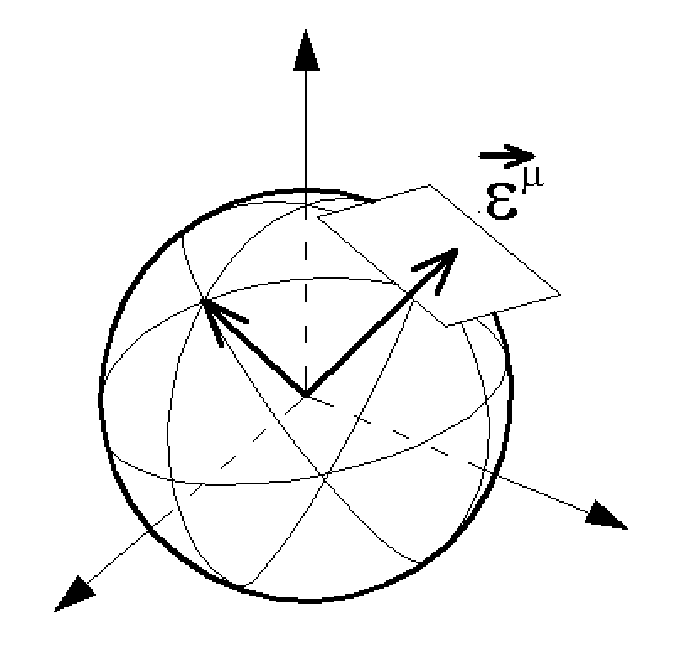
\epsfig{file=sphere.eps,width=70mm}
\caption{Definition of microplanes.}
\label{fig:sphere1}
\end{figure}
\begin{figure}[h]
\centering
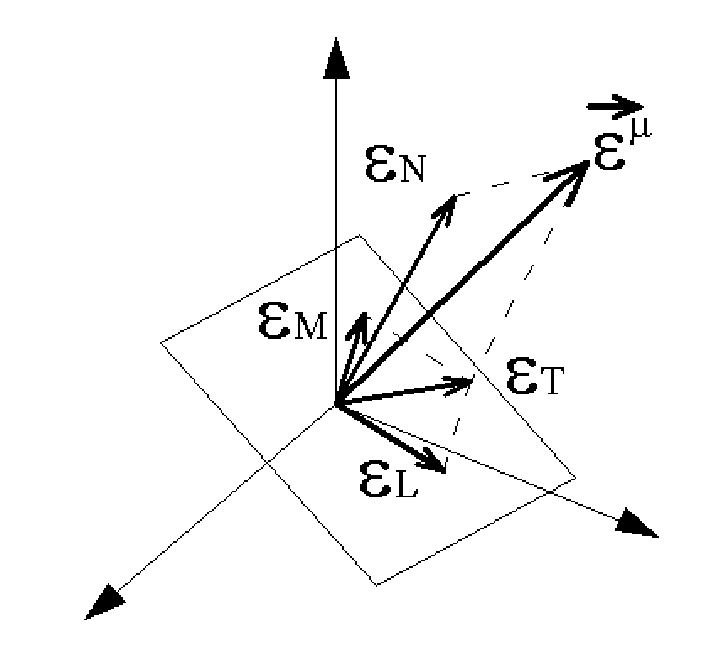
\epsfig{file=cmpnts.eps,width=70mm}
\caption{Definition of microstrain components.}
\label{fig:sphere2}
\end{figure}

Since kinematic constraint (projection of $\varepsilon_{ij}$) was adopted, microplane stress components cannot
be in general equal to projection of macrostress tensor $\sigma_{ij}$. Static equivalence between microstress
and macrostress is ensured by means of the principal of virtual work.
Virtual work of macroscopic stress tensor working on virtual macrostrains within the unit sphere $\Omega$ of volume $\frac{4}{3}\pi$
\begin{equation}
\label{Wmacro}
W^{macro} = \int_\Omega \sigma_{ij} \delta\varepsilon_{ij}d\Omega=\frac{4\pi}{3}\sigma_{ij}\delta\varepsilon_{ij}
\end{equation}
must be equal to the work of all microstress components working on virtual microstrains (normal and shear) integrated over the surface of the
unit sphere, i.e. over all microplanes. Taking into account the symmetry of projection tensors 
it is possible to calculate only with the unit hemisphere $\Gamma$
\begin{equation}
\label{Wmicro}
W^{micro} = 2 \int_\Gamma \left(\sigma_{N} \delta\varepsilon_{N}+ \sigma_M\delta\varepsilon_M + \sigma_L\delta\varepsilon_L\right) d\Gamma.
\end{equation}
Equality of Eq.(\ref{Wmacro}) and Eq.(\ref{Wmicro}) reads macroscopic stress tensor as
\begin{equation}
\label{sij}
\sigma_{ij} = {{3}\over{2\pi}} \int_\Gamma \left(\sigma_N N_{ij} + \sigma_M M_{ij} + \sigma_L L_{ij}\right)d\Gamma.
\end{equation}
Full derivation and details of numerical evaluation of the integral in Eq.(\ref{sij}) 
can be found in \cite{bazant1}, \cite{bazant2} and \cite{bazant3}. 

It is also convenient to use work-conjugate formulation for volumetric stress analogically to formulation of macrostress tensor $\sigma_{ij}$.
Relation for volumetric stress is then given by
\begin{equation}
\label{volstress}
{{2\pi}\over{3}}{{\sigma_{kk}}\over{3}}\delta\varepsilon_{mm} = \int_\Gamma \sigma_V \delta\varepsilon_Vd\Gamma.
\end{equation}
Using projection tensors for microstrains yields final equation for macroscopic stress tensor as
\begin{equation}
\label{sid}
\sigma_{ij} = \sigma_V\delta_{ij} + {{3}\over{2\pi}}\int_\Gamma \left(\sigma_D \left(N_{ij} -
{{\delta_{ij}}\over{3}}\right) + \sigma_M M_{ij} + \sigma_L L_{ij}\right) d\Gamma.
\end{equation}


Constitutive relations between microstrains and microstresses can be defined in different ways.
An intensive development in this area was undertaken at Northwestern University (Prof. Ba\v{z}ant). 
Microplane model M4  uses concept of so called stress-strain boundaries. 
In the computational implementation, at first the elastic prediction of microstresses is computed and this 
prediction is corrected by the relevant boundary stresses.

Constitutive relations  of model M4 contain  a significant number
of  fixed  parameters  $c_i$  that  have  been  gained by fitting of
various  laboratory test  results. Parameters $k_i$ have  to be set
according  to  the  particular   case.  Parameters $c$  have  been
determined as  $c_1 = 6.20, c_2 = 2.76, c_3 = 4.00,  c_4 = 70,
c_5 =2.50, c_6 = 1.30,  c_7 = 50, c_8 = 8.00, c_9 =  1.30, c_{10} = 0.73,
c_{11} = 0.20, c_{12} = 7000, c_{13} = 0.23, c_{14} = 0.80, c_{15} = 1,
c_{16} = 0.02,c_{17} = 0.01, c_{18} =  1, c_{19} = 0.40,  c_{20} =  14.$
A typical set of these optional $k-$parameters are  $k_1 = 1.5 \times 10^{-4}, k_2 =  500, k_3 =  15, k_4 = 150.$
Optional  parameters vary  approximately in  the following ranges:\\
$0.8 \times 10^{-4} \le  k_1 \le 2.5 \times 10^{-4}$,\\
$100 \le k_2 \le 1000$,\\
$5 \le  k_3 \le 15$,\\
$ 30  \le k_4 \le 200$.

%%%%%%%%%%%%%%%%%%%%%%%%%%%%%%%%%%%%%%%%%%%%%%%%%%%%%%%%%%%%%%%%%%%%%%%%%%%%%%%%%%%%%
%%%%%%%%%%%%%%%%%%%%%%%%%%%%%%%%%%%%%%%%%%%%%%%%%%%%%%%%%%%%%%%%%%%%%%%%%%%%%%%%%%%%%
%%%%%%%%%%%%%%%%%%%%%%%%%%%%%%%%%%%%%%%%%%%%%%%%%%%%%%%%%%%%%%%%%%%%%%%%%%%%%%%%%%%%%
%%%%%%%%%%%%%%%%%%%%%%%%%%%%%%%%%%%%%%%%%%%%%%%%%%%%%%%%%%%%%%%%%%%%%%%%%%%%%%%%%%%%%
\section{Damage material models}
\label{sectdammatmodels}
\index{material!damage}\index{damage model}

%%%%%%%%%%%%%%%%%%%%%%%%%%%%%%%%%%%%%%%%%%%%%%%%%%%%%%%%%%%%%%%%%%%%%%%%%%%%%%%%%%%%%
%%%%%%%%%%%%%%%%%%%%%%%%%%%%%%%%%%%%%%%%%%%%%%%%%%%%%%%%%%%%%%%%%%%%%%%%%%%%%%%%%%%%%
\subsection{Isotropic damage models}
\index{material!damage!isotropic}

Isotropic damage models are popular for their simplicity. Only one parameter
describes damage of the material.

The constitutive relation with influence of isotropic damage has form
\begin{equation}
\sigma_{ij} = (1-\omega) D_{ijkl} \varepsilon_{kl}\ ,\ \ \ \ \ \
\mbf{\sigma} = (1-\omega) \mbf{D} \mbf{\varepsilon}\ ,
\end{equation}
where $\omega$ denotes damage \index{damage parameter} parameter. The damage parameter is defined
by relations
\begin{equation}
\omega = g (\tilde{\varepsilon})
\end{equation}
where $\tilde{\varepsilon}$ stands for the equivalent \index{equivalent strain} strain. There are many definitions
of this strain.

\begin {itemize}
\item{
strain norm:\index{norm!strain}
\begin{equation}\label{eqnorstrain}
\tilde{\varepsilon} = \sqrt{\varepsilon_{ij}\varepsilon_{ij}} =
\sqrt{\mbf{\varepsilon}^T \mbf{P} \mbf{\varepsilon}}\ ,
\end{equation}
}
\item{
energy norm:\index{norm!energy}
\begin{equation}\label{eqnorenergy}
\tilde{\varepsilon} = c\sqrt{\varepsilon_{ij} D_{ijkl} \varepsilon_{kl}} =
\sqrt{\mbf{\varepsilon}^T \mbf{D} \mbf{\varepsilon}}\ ,
\end{equation}
}
\item{
positive strain norm:\index{norm!positive strain}
\begin{equation}\label{eqnorposstrain}
\tilde{\varepsilon} = \sqrt{\langle\varepsilon_{ij}\rangle\langle\varepsilon_{ij}\rangle} =
\sqrt{\langle\mbf{\varepsilon}\rangle^T \mbf{P} \langle\mbf{\varepsilon}\rangle}\ ,
\end{equation}
where $\langle \rangle$ denotes the positive part of argument,
}
\item{
positive energy norm:\index{norm!positive energy}
\begin{equation}\label{eqnorposenergy}
\tilde{\varepsilon} = c\sqrt{\langle\varepsilon_{ij}\rangle D_{ijkl} \langle\varepsilon_{kl}\rangle} =
\sqrt{\langle\mbf{\varepsilon}\rangle^T \mbf{D} \langle\mbf{\varepsilon}\rangle}\ ,
\end{equation}
}
\item{
Rankine norm :\index{norm!Rankine}
\begin{equation}\label{eqnorrankine}
\tilde{\varepsilon}=\del{\sqrt{max(\sigma_I) max(\sigma_I)}}{E},
\end{equation}
where $max(\sigma_I)$ is maximal positive value of principal stresses and $E$ is Young modulus,
}
\item{
smothed Rankine norm :\index{norm!smothed Rankine}
\begin{equation}\label{eqnorrankinesmooth}
\tilde{\varepsilon} = \del{\sqrt{\langle\sigma_I\rangle\langle\sigma_I\rangle}}{E},
\end{equation}
}
\item{
Mazar norm :\index{norm!Mazar}
\begin{equation}\label{eqnormazar}
\tilde{\varepsilon} = \sqrt{\langle\varepsilon_I\rangle \langle\varepsilon_I\rangle},
\end{equation}
where $\varepsilon_I$ are principal strains,
}
\item{
von Mises norm :\index{norm!von Mises}
\begin{equation}\label{eqnorvonmises}
\tilde{\varepsilon} = \del{k-1}{2k(1-2\nu)}I_1+\del{1}{2k}\sqrt{\del{(k-1)^2}{(1-2\nu)^2}I_1^2 - \del{12k}{(1+\nu)^2}J_2}
\end{equation}
where k is ration between uni-axial compressive and uniaxial tensile strength. $I_1$ and $J_2$ are the first invariant of
the strain tensor and the second invariant of the deviatoric strain tensor respectively.
}
\end {itemize}

\subsection{Numerical algorithm}
\begin{center}
\begin{tabular}{|l|ll|}
\hline
new strains & \multicolumn{2}{l|}{$\mbf{\varepsilon}_{n+1}=\mbf{\varepsilon}_{n} + \Delta\mbf{\varepsilon}_{n}$}
\\[3mm]
equivalent strain & \multicolumn{2}{l|}{$\tilde{\varepsilon}_{n+1}=\tilde{\varepsilon}(\mbf{\varepsilon})$}
\\[3mm]
parameter $\kappa$ & if $\tilde{\varepsilon}_{n+1}>\kappa_n$ & then $\kappa_{n+1}=\tilde{\varepsilon}_{n+1}$
\\[3mm]
 & & else $\kappa_{n+1}=\kappa_n$
\\[3mm]
damage parameter & \multicolumn{2}{l|}{$\omega_{n+1} = g(\kappa_{n+1})$}
\\[3mm]
new stress & \multicolumn{2}{l|}{$\mbf{\sigma}_{n+1}=(1-\omega_{n+1})\mbf{D} \mbf{\varepsilon}_{n+1}$}
\\ \hline
\end{tabular}
\end{center}

%%%%%%%%%%%%%%%%%%%%%%%%%%%%%%%%%%%%%%%%%%%%%%%%%%%%%%%%%%%%%%%%%%%%%%%
%%%%%%%%%%%%%%%%%%%%%%%%%%%%%%%%%%%%%%%%%%%%%%%%%%%%%%%%%%%%%%%%%%%%%%%
\subsection {Scalar isotropic damage}
\label{theoscdam}

Material parameters of the scalar isotropic damage model are:
\begin{itemize}
\item[]{$d_0$ - intial value of the damage variable $d$,}
\item[]{$\sigma_t$ -  the tensile strength,}
\item[]{$u_f$  -  determines the softening, therefore it corresponds to crack opening (not strain) when tension stress vanishes}
\item[]{$c$ -  the coefficient which is used when damage function parameters are computed as the energy norm.
(This parameter is used due to obtain correct units of the damage function parameter {\it kappa})}
\end{itemize}

This model is based on two relationships. The first one is the relation between stress, $\sigma$, and crack opening, $u$,
\begin{equation}
\sigma = f(u) = \sigma_t exp(-u/u_f)\ ,
\end{equation}
where $\sigma_t$ denotes the tensile strength \index{tensile strength} and 
$u_f$ determines the softening - corresponds to crack opening (not strain) when tension stress vanishes.

The second one is stress/strain relation,
\begin{equation}
\sigma=(1 - d) E \varepsilon
\end{equation}
where $d$ is damage variable.

The scalar damage model depends on the mesh because decreasing size of elements leads to decreasing amount of
dissaipated energy. Theoretically, the zero element size means no dissipated energy in damaged material which is
nonsence from the physical point of view. The dissipated energy during damage process can be assumed as a material
parameter and the model have to capture it. For this purpose, the following modification of the model is used in the code.

The fracture \index{fracture energy} energy, $G_f$, can be expressed in the form
\begin{equation}
G_f = \int_0^{\infty} \sigma_t e^{-{u \over u_f}} {\rm d}u = \sigma_t u_f\ .
\end{equation}
For example, fracture energy of concrete is in the range 65 - 200 N/m. Additional condition
\begin{equation}\label{eqnscdamcons}
\varepsilon^{e} = \del{\sigma_t}{E} < \del{u_f}{h}
\end{equation}
must be satisfied. The following notation is used in the equation (\ref{eqnscdamcons}):
$\varepsilon^{e}$ denotes the limit elastic strain, $\sigma_t$ stands for the tensile strength and $h$
expresses the generalized element size. The generalized element size is defined by
\begin{equation}
h = l\ ,
\end{equation}
\begin{equation}
h = \sqrt{A}\ ,
\end{equation}
\begin{equation}
h = \root 3 \of {V}\ ,
\end{equation}
where $l$ is the length of 1D element, $A$ denotes the area of 2D element and $V$ expresses the volume of 3D element.

Supposing $\tilde{\varepsilon} - \varepsilon_e \approx u/h$ and with respect to the relation $\varepsilon_e = \sigma/E$, one can write
\begin{eqnarray}
\sigma&=&(1 - d) E \tilde{\varepsilon} = f(h(\tilde{\varepsilon}-\sigma/E))
\\
(1 - d) E \tilde{\varepsilon} &=& f(h(\tilde{\varepsilon}-((1-d) E \tilde{\varepsilon})/E))
\\
(1 - d) E \tilde{\varepsilon} &=& f(h d \tilde{\varepsilon})
\\
\label{eqnscdamparam}
0 &=& (1 - d) E \tilde{\varepsilon} - f(h d \tilde{\varepsilon})
\end{eqnarray}

The unknown variable $d$ is solved from the equation (\ref{eqnscdamparam}), where
$h$ stands for the size of element.  The element lenght is used for 1D problem while $h = \sqrt{A}$ is valid for
2D problem. $A$ denotes the area of the element. The Newton method is used for the solution of (\ref{eqnscdamparam})
because the equation is nonlinear and the exact solution is not generally known.

\subsection{Scalar isotropic damage with crack closure}
This model has been implemented by virtue of paper Continuum damage modelling and some computational issues (G. Pijaudier-Cabot,
Ludovic Jason, RFGC - 6/2002 Numerical Modelling in Geomechanics), section 2.3 Integrated Damage Model.
%%%%%%%%%%%%%%%%%%%%%%%%%%%%%%%%%%%%%%%%%%%%%%%%%%%%%%%%%%%%%%%%%%%%%%%%%%%%%%%%%%%%%
%%%%%%%%%%%%%%%%%%%%%%%%%%%%%%%%%%%%%%%%%%%%%%%%%%%%%%%%%%%%%%%%%%%%%%%%%%%%%%%%%%%%%
%%%%%%%%%%%%%%%%%%%%%%%%%%%%%%%%%%%%%%%%%%%%%%%%%%%%%%%%%%%%%%%%%%%%%%%%%%%%%%%%%%%%%
%%%%%%%%%%%%%%%%%%%%%%%%%%%%%%%%%%%%%%%%%%%%%%%%%%%%%%%%%%%%%%%%%%%%%%%%%%%%%%%%%%%%%
\section{Visco-plastic material models}
\label{sectvisplasmatmodels}

Additive decomposition \index{additive decomposition} of rate of strain tensor
\begin{equation}
\dot{\varepsilon}_{ij}=\dot{\varepsilon}^e_{ij}+\dot{\varepsilon}^{vp}_{ij},
\label{eq:adddecomp}
\end{equation}
is used in cases of small strains. $\dot{\varepsilon}^e_{ij}$ means rate of elastic \index{elastic strain tensor} part of the strain tensor
and $\dot{\varepsilon}^{vp}_{ij}$ stands for rate of irreversible, viscoplastic, \index{viscoplastic strain tensor} part of strain tensor.
The loading surface \index{loading surface} $f=0$ is continuous and convex. Perzyna then suggests the constitutive law
for the viscoplastic flow as
\begin{equation}
\dot{\varepsilon}^{vp}_{ij}=\gamma\Bigl\langle\Phi\bigl(f\bigl)\Bigr\rangle\frac{\partial G^*}{\partial\sigma_{ij}},
\label{eq:visplasincr}
\end{equation}
where $\gamma$ is the viscosity coefficient \index{viscosity coefficient} of material, $G^*$ is the visco-plastic
\index{viscoplastic potential} potential and
$\Bigl\langle\Phi\bigl(f\bigl)\Bigr\rangle$ is a flow function \index{flow function}\index{function!flow} containing the loading function $f$.
The function $\Phi$ is controlled by Macauly's \index{Macauly's brackets} brackets
\begin{equation}
{\Bigl\langle\Phi\bigl(f\bigl)\Bigl\rangle=\frac{1}{2}\biggl[\Phi\bigl(f\bigr)+\Bigl|\Phi\bigl(f\bigr)\Bigr|\biggr]}.
\end{equation}
Useful variable is cumulative viscoplastic strain \index{cumulative viscoplastic strain} which is defined as
\begin{equation}
\varepsilon^{vp}(t)=\displaystyle\int_0^t\sqrt{\frac{2}{3}\dot{\varepsilon}^{vp}_{ij}\dot{\varepsilon}^{vp}_{ij}}\ {\rm d}t.
\label{eq:cumulvisplas}
\end{equation}


Viscoplastic problems depend on time and therefore modified equation of equilibrium
is used for derivation of discrete system. It is convenient to start from the time derivative
of equilibrium condition
\begin{equation}\label{equilibcond}
\mbf{\partial} \dot{\mbf{\sigma}} + \dot{\mbf{X}} = \mbf{0} \ .
\end{equation}
After premultiplying of previous equation by test function and using standard finite
element approximation
\begin{equation}\label{femappr}
\mbf{u}=\mbf{N} \mbf{r}\ , \ \ \ \ \ \
\mbf{\varepsilon} = \mbf{B} \mbf{r}
\end{equation}
the equilibrium condition (\ref{equilibcond}) can be rewritten to the form
\begin{equation}\label{dicrequilibcond}
\delta \mbf{r}^T \left(\int_{V} \mbf{B}^T \dot{\mbf{\sigma}}\ {\rm d}V -
\int_{V} \mbf{N}^T \mbf{N} \dot{\mbf{w}}\ {\rm d}V -
\int_{S} \mbf{N}^T \mbf{N} \dot{\mbf{p}}\ {\rm d}S
\right)=0
\end{equation}
where $\mbf{w}$ is vector of volume forces, $\mbf{p}$ is vector of boundary tractions,
$\mbf{N}$ is the matrix of approximation functions and $\mbf{B}$ is matrix of derivatives
of approximation functions ($\mbf{B}=\mbf{\partial}\mbf{N}$). The constitutive relation
of viscoplastic problems is formulated in rate form
\begin{equation}\label{constrel}
\dot{\mbf{\sigma}} = \mbf{D} (\dot{\mbf{\varepsilon}} - \dot{\mbf{\varepsilon}}_{vp}) \ .
\end{equation}
When the relation (\ref{constrel}) is used in equation (\ref{dicrequilibcond}), the
ordinary differential equation is obtained and can be written as
\begin{equation}\label{algdiffeq}
\mbf{K} \dot{\mbf{r}} = \dot{\mbf{f}} +
\int_{V} \mbf{B}^T \mbf{D} \dot{\mbf{\varepsilon}}_{vp}\ {\rm d}V
\end{equation}
where the usual notation for stiffness matrix
\begin{equation}
\mbf{K} = \int_{V} \mbf{B}^T \mbf{D} \mbf{B}\ {\rm d}V
\end{equation}
and load forces
\begin{equation}
\mbf{f}=\int_{V} \mbf{N}^T \mbf{N} \mbf{w}\ {\rm d}V +
\int_{S} \mbf{N}^T \mbf{N} \mbf{p}\ {\rm d}S
\end{equation}
is used.

We use explicit algorithm for solution of equation (\ref{algdiffeq}) which is based on
replacement of time derivatives by finite differences what results in form
\begin{equation}\label{fullydiscr}
\mbf{K} \Delta \mbf{r} = \Delta \mbf{f} + \int_{V} \mbf{B}^T \mbf{D} \Delta \mbf{\varepsilon}_{vp}\ {\rm d}V \ .
\end{equation}
The previous equation does not have any derivatives and is solved in iterative loop.

The following quantities are known at time $t=t_i$: stresses $\mbf{\sigma}_i$, displacement
vector $\mbf{r}_i$, irreversible strains $\mbf{\varepsilon}_{vp}$. Do following steps until $t_i=t_{required}$:

\begin{center}
\begin{tabular}{|l|l|}
\hline
\multicolumn{2}{|c|}{Iterate until $t \leq t_{required}$}
\\ \hline
overstress (defined by yield function) &
$(\sigma_{over})_i = f(\mbf{\sigma}_i)$
\\[3mm]
increment of viscoplastic strain &
$(\Delta \mbf{\varepsilon}_{vp})_i = \Delta t \gamma\Bigl\langle\Phi\bigl(f\bigl)\Bigr\rangle\frac{\partial G^*}{\partial\sigma_{ij}}$
\\[3mm]
increments of internal nodal forces &
$(\Delta \mbf{f}_{ir})_{i+1} = \int_{V} \mbf{B}^T \mbf{D} (\Delta \mbf{\varepsilon}_{vp})_i\ {\rm d}V$
\\[3mm]
increments of external nodal forces &
$(\Delta \mbf{f})_{i+1} = \mbf{f}(t_{i+1})-\mbf{f}(t_i)$
\\[3mm]
increments of displacements &
$(\Delta \mbf{r})_{i+1} = \mbf{K}^{-1} ((\Delta \mbf{f})_{i+1} + (\Delta \mbf{f}_{ir})_{i+1})$
\\[3mm]
new vector of displacements &
$\mbf{r}_{i+1} = \mbf{r}_{i} + \Delta \mbf{r}_{i+1}$
\\[3mm]
total strain increments &
$(\Delta \mbf{\varepsilon})_{i+1}=\mbf{B}\mbf{r}_{i+1}-\mbf{\varepsilon}_{i}$
\\[1mm]
(previous total strain $\mbf{\varepsilon}_{i}$ is stored) &
\\[3mm]
stress increments &
$(\Delta \mbf{\sigma})_{i+1}=\mbf{D} ((\Delta \mbf{\varepsilon})_{i+1} - (\Delta \mbf{\varepsilon}_{vp})_i)$
\\[3mm]
new stresses &
$\mbf{\sigma}_{i+1} = \mbf{\sigma}_{i}+(\Delta \mbf{\sigma})_{i+1}$
\\ \hline
\end{tabular}
\end{center}

As was mentioned before, the presented algorithm is explicit one and therefore the time step
must be choosen carefully.
For more details about numerical solution of equation (\ref{fullydiscr}) and about numerical stability
of the algorithm see e.g. \cite{Plesek} and \cite{Cormeau}.

\subsection{Lemaitre model of viscosity}
\label{sectlemaitremodel}


%%%%%%%%%%%%%%%%%%%%%%%%%%%%%%%%%%%%%%%%%%%%%%%%%%%%%%%%%%%%%%
%%%%%%%%%%%%%%%%%%%%%%%%%%%%%%%%%%%%%%%%%%%%%%%%%%%%%%%%%%%%%%
%%%%%%%%%%%%%%%%%%%%%%%%%%%%%%%%%%%%%%%%%%%%%%%%%%%%%%%%%%%%%%
%%%%%%%%%%%%%%%%%%%%%%%%%%%%%%%%%%%%%%%%%%%%%%%%%%%%%%%%%%%%%%
\section{Creep}
\index{material!creep}

Method of solving

The basic idea is in conversion integral equation to differential. Boltzman principle \index{Boltzman principle} of superposition
for strain is given by integral equation

\begin{equation}
\varepsilon(t) = J(t,t_0)\sigma + \int_{t_0}^{t} {J(t,\tau) {\rm d}\sigma(\tau)} + \varepsilon_0(t)\ ,
\end{equation}
where $J(t,t_0)$ is creep \index{creep function}\index{function!creep} function.
Creep function is necessary to express for conversion in the form
\begin{equation}
J(t,\tau) = \sum_{\mu=1}^{M} \frac{1}{D_\mu(\tau)} \{{1-e^{y_\mu(\tau)-y_{\mu}(t)}}\} 
\end{equation}
\begin{equation}
y_{\mu}(t) = \left({\frac{t}{\tau_\mu}}\right)^{\frac{2}{3}}
\end{equation}
$\tau_\mu$ are retardation \index{retardation times} times,
$D_\mu(\tau)$ are coefficients for members of Dirichlet series \index{Dirichlet series} obtain from creep function
\\
The whole strain is
\begin{equation}
\varepsilon(t) = \sum_{\mu=1}^{M}  \int_{\Delta t} \frac{{\rm d}\sigma(\tau)}{D_\mu(\tau)}- \gamma_{\mu}(t) + \varepsilon_0(t) 
\end{equation}

Diferential equations are
\begin{equation}
\frac{d\gamma_\mu(t)}{dy_\mu(t)} + \gamma_{\mu}(t) =  \frac{1}{D_{\mu}(t)} \frac{{\rm d}\sigma(t)}{dy_{\mu}(t)} 
\end{equation}
\begin{equation}
\frac{d\varepsilon_\mu(t)}{dy_\mu(t)}=\gamma_\mu(t) 
\end{equation}


\begin{center}
Calculation procedure

\begin{tabular}{|l|l|}
\hline
set of retardation times &
$\tau_\mu$, where $\mu \in \{1,\ 2,\ \ldots,\ 7\}$
\\[3mm]
initial values &
$\mbf{\gamma}_\mu(0)=0,\ \ \mbf{\sigma}(0)=0,\ \ \mbf{\varepsilon}(0)=0,\ \ \mbf{u}(0)=0$
\\[3mm] \hline
\multicolumn{2}{|c|}{Iterate}
\\[3mm] \hline
increment of load &
$\Delta \mbf{R}^f$
\\[3mm]
increment of strains &
$\Delta\overline{\varepsilon} = \sum_{\mu=1}^{M} {\gamma_{\mu}(t_{i-1})(1-e^{-\Delta y_\mu})}$
\\[3mm]
compute forces &
$\Delta \mbf{R}^c (\Delta\overline{\varepsilon})$
%B.3  Change deformation $\Delta\overline{\varepsilon}$ to forces $\Delta \mbf{R}^c$
\\[3mm]
coefficients of Dirichlet series &
$C_\mu(t_{(i+1/2)})$ from creep function $J(t,t_{(i+1/2)})$
\\[3mm]
assambling of stiffnes matrix &
$\mbf{K}$
\\[3mm]
 &
$\Delta\mbf{\sigma}_i = {\overline{E}\overline{\mbf{D}}} (\Delta\varepsilon_i-\overline{\Delta\varepsilon_i}-\Delta\varepsilon_{(0i)})$
\\[3mm]
 &
$\frac{1}{\overline{E}} = \sum_{\mu=1}^{M} {\frac{1-\lambda_{\mu}}{C_{\mu}(t_{(i+1/2)})}}$
\\[3mm]
increment of displacements &
$\mbf{K} \Delta  \mbf{u}_i = \Delta \mbf{R}^f + \Delta \mbf{R}^c$
\\[3mm]
increment of strains &
$\Delta\mbf{\varepsilon}_i = \mbf{B} \Delta \mbf{u}_i$
\\[3mm]
increment of stresses &
$\Delta\mbf{\sigma}_i = {\overline{E}\overline{\mbf{D}}} (\Delta\varepsilon_i-\overline{\Delta\varepsilon_i}-\Delta\varepsilon_{(0i)})$
\\[3mm]
internal values &
$\mbf{\gamma}_\mu(t_i) = \mbf{\gamma}_\mu (t_{i-1}) e^{-\Delta y_\mu} + \frac{\overline{\mbf{C}}} {\overline{D_\mu}(t+1/2)}
{\frac{1-e^{-\Delta y_\mu}}{\Delta y_\mu} }  \Delta\mbf{\sigma}_i$
\\ \hline
\end{tabular}
\end{center}

%%%%%%%%%%%%%%%%%%%%%%%%%%%%%%%%%%%%%%%%%%%%%%%%%%%%%%%%%%%%%%%%%
\subsection{B3 model}
Creep function B3
\index{!creep!bazant}  Bazant, Baweja - Model B3- Rilem recom. Mater. Structures 1995
\\\begin{eqnarray}
J(t,\tau) &=& q_1 + q_2 Q(t,\tau) + q_3 \ln{ \left( 1+(t-\tau)^n \right)} + q_3 \ln{(t/\tau)}
\\ \nonumber
&+& q_4\sqrt{ exp{\left( 8(1-h)\tanh{ \sqrt{\frac{t-t_0}{\tau_{sh}} } } - 8  \right)} - exp{\left( 8(1-h)\tanh{ \sqrt{\frac{\tau-t_0}{\tau_{sh}} } } - 8  \right)}  }
\end{eqnarray}


\begin{equation}
q_1 = \frac{600000}{E_{28}}
\end{equation}
where $E_{28} = 4734 \sqrt{f_c} $, $f_c $ is elastic modulus for 28 days
$h$ is humidity\index{humidity}


\begin{equation}
q_2 = 185,4 \sqrt{c} f^{-0,9}_c
\end{equation}


\begin{equation}
Q(t,\tau) = \left(0,086 \tau^{2/9} + 1,21 \tau^{4/9} \right)^{-1}  
\left( 1 + \left( \frac{ \left(0,086 \tau^{2/9} + 1,21 \tau^{4/9} \right)^{-1} } 
{\tau^{-m} \ln {\left( 1 + (t- \tau)^n \right) } } \right)^{r_\tau } \right)^{\frac{-1}{r_\tau}} 
\end{equation}


where $ r_\tau = 1,7 \tau^{0,12} +8 $

$m, n$ are material's constants $m=0.5, n=0.1$

\begin{equation}
q_3 = 0,29 (w/c)^4  q_2
\end{equation}


\begin{equation}
q_4 = 20,3 (a/c)^{-0,7}
\end{equation}
\\


Components of material

\begin{center}
\begin{tabular}{|l|l}
\hline
$h_s = 0.4$ & humidity
\\  
$k_s = 1.0$ & shape factor \index{shape factor}  slab=1.0, cylinder=1.15, sguare prism.=1.25, sphere=1.3, cube=1.55
\\
$tl = 0.12$ & effective cross section thickness       $D=2*vs_s$
%
%  from t0  to t 
%
%  from concrete starts   tb 
\\
$t_w$ & age when drying begins
\\
$fc'$ & 28 day average cylinder strenght \index{average cylinder strenght} fc' [MPa]
\\
 & (original from Bazant [ksi]) ksi=1000psi=6.895MPa (f.e.6.454=44.5MPa)
\\
$w/c$ & water-cement ratio \index{water-cement ratio}\index{ratio!water-cement} of the mix by weight   ***0.43
\\
$s/c$ & send-cement ratio \index{send-cement ratio}\index{ratio!send-cement} of the mix by weight    ***3.4
\\
$g/c$ & gravel-cement ratio \index{gravel-cement ratio}\index{ratio!gravel-cement} of the mix by weight $g/c=a/c-s/c$     ***1.98
\\
$a/c$ & aggregate-cement ratio \index{aggregate-cement ratio}\index{ratio!aggregate-cement} of the mix by weight $a/c=g/c+s/c$
\\
$a1$ & coef. for cements of type I,II a1=1.00, III a1=0.93, IV a1=1.05   ***1.05
\\
$ro$ & mass of concrete in [kg/m3]   (original from Bazant[lb/ft3]) [lb/ft3]=16.03 kg/m3 ***156
\\
$cs$ & cement content in m3  .. kg/m3
\\
$E28=4734 fc'$ &
\\
$Et=E_{28} \sqrt{(t/(4+0.85*t))}$ & with respect to ACI Commite 209/II
\\ \hline
\end{tabular}
\end{center}

%%%%%%%%%%%%%%%%%%%%%%%%%%%%%%%%%%%%%%%%%%%%%%%%%%%%%%%%%%%%%%
%%%%%%%%%%%%%%%%%%%%%%%%%%%%%%%%%%%%%%%%%%%%%%%%%%%%%%%%%%%%%%
\section{Consolidation}
\index{Terzaghi consolidation}\index{material!consolidation}\index{material!consolidation!Terzaghi}
one-dimensional consolidation

Method of solving
\\
Terzaghi theory one dimensional consolidation. The soil is full under wather. The bottom
soil in depth $h$ is wather proof.
\begin{equation}
\ppd{p}{t} = c_v \npd{2}{p}{z}\ ,
\end{equation}
where
\begin{equation}
c_v =\frac{k E_{oed}}{\gamma_w}
\end{equation}
$k$ is coefficient of consolidation \index{coefficient of consolidation}\index{coefficient!consolidation} from 1 to $10^{-3} m/day$
$\gamma_w = 10 kN/m^3$ 
$E_{oed}$ is edometrics modulus \index{modulus!edometric}\index{edometric modulus}
solving differential equation is found in series
\begin{equation}
p(t,z) = \frac{4f}{\pi} \sum_{\mu=1,3,5...}^{M} \frac{1}{\mu}
e^{-\left(\frac{\pi \mu}{2h}\right)^2} c_v t\ sin\frac{\pi \mu z}{2h}
\end{equation}

\begin{equation}
\varepsilon(t) = \frac{1}{E_{oed}} \left(U(t-t_0)f(t_0) + \int_{t_0}^{t} U(t-\tau){\rm d}f(\tau)\right)
\end{equation}
From mathemathics point of wiev is $U$ similar as $J$ in creep 
\begin{equation}
U(t,\tau) =   \sum_{\mu=1,3,5...}^{M} \frac{8}{\pi^2 \mu^2}
\left[1 - e^{-\left(\frac{\pi\mu}{2h}\right)^{2} c_v (t-\tau)}\right]
\end{equation}




Calculation procedure
A.1  Set of number of members series  $\mu$ is only odd
     $\mu$ .... from 1 to 7
A.2  Set of showen values $ \mbf{\gamma}_\mu(0)=0, \mbf{\sigma}(0)=0, \mbf{\varepsilon}(0)=0, \mbf{u}(0)=0.$

Steps for each time $t_i$

B.1  Increment of loadings $\Delta \mbf{R}^f$

B.2  Computing of deformation from consol

\begin{equation}
\Delta\overline{w} = \sum_{\mu=1}^{M} {\gamma_{\mu}(t_{i-1})(1-e^{-\Delta y_\mu})}
\end{equation}

B.3  Change deformation $\Delta\overline{w}$ to forces $\Delta \mbf{R}^w$

\begin{equation}
\Delta R^w = -\mbf{K} \left[  \sum_{\mu=1,3,5...}^{M} \frac{8}{\pi^2 \mu^2}
(1 - \frac{1-e^{\Delta y_{\mu}}} {\Delta y_{\mu}})  \right]^{-1} \Delta\overline{w}
\end{equation}


B.4  Assamble stiffnes matrix $\mbf{K}$ , where $D$,is matrix of soil parameters
\begin{equation}
\mbf{K}_e = \int_v^{}[B]^T 
\left[D \right]
\left[B \right]dV
\end{equation}
     
\begin{equation}
\mbf{K} = \mbf{K}_e \left[ \sum_{\mu=1,3,5...}^{M} \frac{8}{\pi^2 \mu^2}
(1 - \frac{1-e^{-\Delta y_{\mu}}} {\Delta y_{\mu}}) \right]^{-1} 
\end{equation}
     
B.5 Computing increment of displacement
\begin{equation}
\mbf{K} \Delta  \mbf{u}_i = \Delta \mbf{R}^f + \Delta \mbf{R}^w
\end{equation}


B.6 Computing increment of deformations
\begin{equation}
\Delta\mbf{w}_i = \mbf{w}_{i-1} + \Delta \mbf{w}_i
\end{equation}


B.7 Computing increment of forces
\begin{equation}
\Delta\mbf{R}_i = {\mbf{K}_e} \left[ {\sum_{\mu=1,3,5...}^{M} \frac{8}{\pi^2\mu^2}(1-\frac{1-e^{-\Delta y_\mu}} {\Delta y_\mu } )} \right]^{-1} 
(\Delta w_i-\Delta\overline{w}_i)
\end{equation}


B.8 Set of showen values
\begin{equation}
\mbf{\gamma}_\mu(t_i) = \mbf{\gamma}_\mu (t_{i-1}) e^{-\Delta y_\mu} + \frac{8} {\pi^2\mu^2}
{\frac{1-e^{-\Delta y_\mu}}{\Delta y_\mu} } \mbf{K}^{-1}_e \Delta\mbf{R}_i
\end{equation}


B.9  if $t_i<t$ goto B.1. else END
\\


\begin{equation}
\Delta y_\mu = (\frac{\pi\mu}{2h} )^2 c_v t   {\mu=1,3,5...}
\end{equation}


Components of material



  $c_v = 0.002$ ;    koeficient of consolidation []
  
  $h= 2.5$ ;       active deep [m]


  from t0  to t 


\section{Subsoil models}

\subsection{Winkler model}
where $c_1$ is soil parameter
stiffnes of soil
\begin{equation}
c_1 = \int_0^{h} E_{oed} \left(\frac{d\psi}{dz}\right)^2 {\rm d}z
\end{equation}

\subsection{Winkler-Pasternak model}
Assumptions are:
\begin{equation}
u=v=0,\ w(x,y,z)=w(x,y,0)\psi(z)\ .
\end{equation}
Strains
\begin{equation}
\varepsilon_z = w \ppd{\psi}{z}\ ,\ \
\gamma_{xz} = \psi \ppd{w}{x}\, 
\gamma_{yz} = \psi \ppd{w}{y}\, 
\end{equation}
Stresses
\begin{equation}
\sigma_z = E_{oed} w \ppd{\psi}{z}\ ,\ \
\tau_{xz} = G \psi \ppd{w}{x}\, 
\tau_{yz} = G \psi \ppd{w}{y}\, 
\end{equation}

\begin{equation}
\mbf{D} = \left[\begin{array}{cc} C_1 & 0 \\  0 & C_2 \end{array} \right]
\end{equation}
where $C_1$, $C_2$ are soil parameters
stiffnes of soil
\begin{equation}
C_1 = \int_0^{h} E_{oed} \left(\frac{d\psi}{dz}\right)^2 {\rm d}z
\end{equation}

shear stiffnes of soil
\begin{equation}
C_2 = \int_0^{h}{G \psi^2 } dz
\end{equation}

Influence of surrounding soil is expressed
\begin{equation}
C_1^{\star} = C_1 + \frac{1}{b} \sqrt{C_1 C_2}
\end{equation}
\begin{equation}
C_2^{\star} = C_2 + \frac{1}{2b} \sqrt{\frac{C_2^3}{C_1}}
\end{equation}
where $b$ is the width of the foundation.

%%%%%%%%%%%%%%%%%%%%%%%%%%%%%%%%%%%%%%%%%%%%%%%%%%%%%%%%%%%%%%%%%%%%%%%%%%%%%%%%%%%%
%%%%%%%%%%%%%%%%%%%%%%%%%%%%%%%%%%%%%%%%%%%%%%%%%%%%%%%%%%%%%%%%%%%%%%%%%%%%%%%%%%%%
\section{Combination of material models}
\label{sectmatmodcomb}

This section is devoted to combinations of mentioned material models. It is very important
topic especially in connection with programming.

Elastic material law expressed by generalized Hook's law is basis of all material models.
Stresses are computed in theory of plasticity from material law
\begin{equation}\label{eqmatcombp}
\mbf{\sigma} = \mbf{D} \left(\mbf{\varepsilon}-\mbf{\varepsilon}^{p}\right) = \mbf{D} \mbf{\varepsilon}^{e}\ ,
\end{equation}
where elastic strains are used. Similar situation is in viscoplasticity, where relation
\begin{equation}\label{eqmatcombvp}
\dot{\mbf{\sigma}} = \mbf{D} \left(\dot{\mbf{\varepsilon}}-\dot{\mbf{\varepsilon}^{vp}}\right) =
\mbf{D} \dot{\mbf{\varepsilon}^{e}}
\end{equation}
is used. Equation (\ref{eqmatcombvp}) is rate form of Equation (\ref{eqmatcombp}). Finally, the damage
models are based on relation
\begin{equation}\label{eqmatcombd}
\mbf{\sigma} = (1-\omega) \mbf{D} \mbf{\varepsilon}\ .
\end{equation}
From Equations (\ref{eqmatcombp}), (\ref{eqmatcombvp}) and (\ref{eqmatcombd}) follows that elastic
material law is present in all inelastic models.

Consider any yield function $f$ or plastic potential $g$ defined in Section \ref{sectplasmatmodels}. They serve for
computation of increment of plastic strains
\begin{equation}
\dot{\mbf{\varepsilon}}^{p} = \dot{\gamma} \ppd{f}{\mbf{\sigma}}\ \ \ \ \ {\rm or}\ \ \ \ \
\dot{\mbf{\varepsilon}}^{p} = \dot{\gamma} \ppd{g}{\mbf{\sigma}}
\end{equation}
in the theory of plasticity. So called overstress $f(\mbf{\sigma})$ is an important ingredient of viscous models
mentioned in Section \ref{sectvisplasmatmodels}.

With respect to previously mentioned connections, material models can be split into following groups:

\begin{itemize}
\item{elastic material models,}
\item{plastic material models,}
\item{viscous material models,}
\item{damage material models.}
\end{itemize}

%\input{nonlinsolver.tex}
\part{Computer implementation}
\input{hangingnodes.tex}
\chapter{Application of the TRFEL}

\section{The most common variables used in TRFEL}

The most common and used variables and their notation are summarized in this section.
This list is definitely not complete.

\begin{center}
\begin{tabular}{|l|l|}
\hline
{\tt napfun} & number of approximated functions on the element
\\ \hline
{\tt nb} & number of blocks
\\ \hline
{\tt ndofe} & number of degrees of freedom defined on element
\\ \hline
{\tt ne} & number of nodes on element
\\ \hline
{\tt ned} & number of edges on element
\\ \hline
{\tt nned} & number of nodes on one edge
\\ \hline
\end{tabular}
\end{center}

%%%%%%%%%%%%%%%%%%%%%%%%%%%%%%%%%%%%%%%%%%%%%%%%%%%%%%%%%
%%%%%%%%%%%%%%%%%%%%%%%%%%%%%%%%%%%%%%%%%%%%%%%%%%%%%%%%%
\section{TRFEL data types}

Description of TRFEL enumerate data types is summarized in this section. 
The TRFEL enumerate data types are used in abundance in the code. They are defined
in the file aliast.h.

%%%%%%%%%%%%%%%%%%%%%%%%%%%%%%%%%%%%%%%%%%%%%%%%%%%%%%%%%%
\subsection{Type {\sf problemtypet}}
\index{type!{\sf problemtypet}}
\label{sectproblemtypet}

This generalized data type defines type of transport problem.
Admissible values of a variable of the {\sf problemtypet} are defined by a list of symbolic constant names (aliases)
and their numerical representation:

\begin{center}
\begin{tabular}{|l|c|l|}
\hline
{\tt stationary\_problem} & 50 & solution of stationary
\\
 & & linear problems
\\ \hline
{\tt nonstationary\_problem} & 60 & solution of nonstationary
\\
 & & linear problems
\\ \hline
{\tt nonlinear\_nonstationary\_problem} & 61 & solution of nonlinear
\\
 & & nonstationary problems
\\ \hline
\end{tabular}
\end{center}

%%%%%%%%%%%%%%%%%%%%%%%%%%%%%%%%%%%%%%%%%%%%%%%%%%%%%%%%%%
\subsection{Type {\sf transmattert}}
\index{type!{\sf transmattert}}
\label{secttransmattert}

This generalized data type defines type of transported materials (media).
Admissible values of a variable of the {\sf transmattert} are defined by a list of symbolic constant names (aliases)
and their numerical representation:

\begin{center}
\begin{tabular}{|l|c|l|}
\hline
{\tt onemedium} & 1 & one medium is considered
\\ \hline
{\tt twomediacoup} & 10 & two media are considered
\\ \hline
{\tt threemediacoup} & 30 & three media are considered
\\ \hline
\end{tabular}
\end{center}

%%%%%%%%%%%%%%%%%%%%%%%%%%%%%%%%%%%%%%%%%%%%%%%%%%%%%%%%%%
\subsection{Type {\sf mednamest}}
\index{type!{\sf mednamest}}
\label{sectmednamest}

This generalized data type defines names of transported materials (media).
Admissible values of a variable of the {\sf mednamest} are defined by a list of symbolic constant names (aliases)
and their numerical representation:

\begin{center}
\begin{tabular}{|l|c|l|}
\hline
{\tt heat} & 1 & heat is transported
\\ \hline
{\tt moisture} & 2 & moisture is transported
\\ \hline
{\tt heat\_moisture} & 10 & heat and moisture are transported
\\ \hline
\end{tabular}
\end{center}

%%%%%%%%%%%%%%%%%%%%%%%%%%%%%%%%%%%%%%%%%%%%%%%%%%%%%%%%%%
\subsection{Type {\sf proptypet}}
\index{type!{\sf proptypet}}
\label{sectproptypet}

This generalized data type defines names of assigned properties used in the transprep source files.
Admissible values of a variable of the {\sf proptypet} are defined by a list of symbolic constant names (aliases)
and their numerical representation:

\begin{center}
\begin{tabular}{|l|c|l|}
\hline
{\tt boundarycondt} & 2 &
\\ \hline
{\tt crosssect} & 4 &
\\ \hline
{\tt eltypet} & 6 &
\\ \hline
{\tt matelt} & 7 &
\\ \hline
{\tt initcondt} & 11 &
\\ \hline
{\tt comcodnumt} & 12 &
\\ \hline
{\tt loadedget} & 13 &
\\ \hline
{\tt loadsource} & 15 &
\\ \hline
\end{tabular}
\end{center}

%%%%%%%%%%%%%%%%%%%%%%%%%%%%%%%%%%%%%%%%%%%%%%%%%%%%%%%%%%
\subsection{Type {\sf elemtypet}}
\index{type!{\sf elemtypet}}
\label{sectelemtypet}

This generalized data type defines type of finite element used in problem.
Admissible values of a variable of the {\sf elemtypet} are defined by a list of symbolic constant names (aliases)
and their numerical representation:

\begin{center}
\begin{tabular}{|l|c|l|}
\hline
{\tt barlint} & 200 & onedimensional element with linear approximation functions
\\ \hline
{\tt barquadt} & 205 & onedimensional element with quadratic approximation functions
\\ \hline
{\tt trlint} & 210 & triangular element with linear approximation functions
\\ \hline
{\tt trlaxisym} & 211 & triangular element with linear approximation functions\\ & & for axisymmetric problems
\\ \hline
{\tt quadlint} & 215 & quadrilateral element with bi-linear approximation functions
\\ \hline
{\tt quadquadt} & 216 & quadrilateral element with bi-quadratic approximation functions
\\ \hline
{\tt quadlaxisym} & 217 & quadrilateral element with bi-linear approximation functions\\ & & for axisymmetric problems
\\ \hline
{\tt lineartett} & 220 & tetrahedral element with linear approximation functions
\\ \hline
{\tt linearhext} & 225 & hexahedral element with tri-linear approximation functions
\\ \hline
{\tt quadratichext} & 226 & hexahedral element with tri-quadratic approximation functions
\\ \hline
\end{tabular}
\end{center}

%%%%%%%%%%%%%%%%%%%%%%%%%%%%%%%%%%%%%%%%%%%%%%%%%%%%%%%%%%
\subsection{Type {\sf mattypet}}
\index{type!{\sf mattypet}}
\label{sectmattypet}

This generalized data type defines type of material.
Admissible values of a variable of the {\sf mattypet} are defined by a list of symbolic constant names (aliases)
and their numerical representation:

\begin{center}
\begin{tabular}{|l|c|l|}
\hline
{\tt isotransmat} & 100 &
\\ \hline
{\tt cernyconcrete} & 101 &
\\ \hline
{\tt bazantpedersen} & 150 &
\\ \hline
{\tt pedersen} & 151 &
\\ \hline
{\tt kunzel} & 155 &
\\ \hline
{\tt concreteB} & 160 &
\\ \hline
{\tt baroghelB} & 161 &
\\ \hline
{\tt C60baroghelB} & 165 &
\\ \hline
{\tt C30baroghelB} & 166 &
\\ \hline
{\tt o30bazantB} & 167 &
\\ \hline
{\tt C60bazantB} & 168 &
\\ \hline
{\tt glasgow} & 170 &
\\ \hline
\end{tabular}
\end{center}


%%%%%%%%%%%%%%%%%%%%%%%%%%%%%%%%%%%%%%%%%%%%%%%%%%%%%%%%%%
\subsection{Type {\sf crsectypet}}
\index{type!{\sf crsectypet}}
\label{sectcrsectypet}

This generalized data type defines type of cross section.
Admissible values of a variable of the {\sf crsectypet} are defined by a list of symbolic constant names (aliases)
and their numerical representation:

\begin{center}
\begin{tabular}{|l|c|l|}
\hline
{\tt nocrosssectiont} & 0 & no cross section
\\ \hline
{\tt crsec1dt} & 1 & cross section for 1D problems
\\ \hline
{\tt crsec2dt} & 2 & cross section for 2D problems
\\ \hline
{\tt crsec3dt} & 3 & cross section for 3D problems
\\ \hline
\end{tabular}
\end{center}

%%%%%%%%%%%%%%%%%%%%%%%%%%%%%%%%%%%%%%%%%%%%%%%%%%%%%%%%%
\subsection{Type {\sf strastret}}
\index{type!{\sf strastret}}
\label{sectstrastret}

This generalized data type defines type of processed quantity.
Admissible values of a variable of the {\sf strastret} are defined by a list of symbolic constant names (aliases)
and their numerical representation:

\begin{center}
\begin{tabular}{|l|c|l|}
\hline
{\tt grad} & 0 & gradients are computed
\\ \hline
{\tt flux} & 1 & fluxes are computed
\\ \hline
{\tt othert} & 2 & other values are computed
\\ \hline
\end{tabular}
\end{center}


%%%%%%%%%%%%%%%%%%%%%%%%%%%%%%%%%%%%%%%%%%%%%%%%%%%%%%%%%%%%
\subsection{Type {\sf graphftt}}
\index{type!{\sf graphftt}}
\label{sectgraphftt}
This generalized data type defines in the output driver which type of
output graphics format is used.

\begin{center}
\begin{tabular}{|l|c|l|}
\hline
{\tt grftt\_no} & 0 & no graphics output
\\ \hline
{\tt grftt\_open\_dx} & 1 & OpenDX format
\\ \hline
{\tt grftt\_gid} & 3 & GID format
\\ \hline
\end{tabular}
\end{center}

%%%%%%%%%%%%%%%%%%%%%%%%%%%%%%%%%%%%%%%%%%%%%%%%%%%%%%%%%%%%
\subsection{Type {\sf prunkt}}
\index{type!{\sf prunkt}}
\label{sectprunkt}
This generalized data type defines in the output diagrams type of
printed unknowns. 

\begin{center}
\begin{tabular}{|l|c|l|}
\hline
{\tt pr\_unknowns} & 1 & unknowns vector
\\ \hline
{\tt pr\_gradients} & 2 & gradients
\\ \hline
{\tt pr\_fluxes} & 3 & fluxes
\\ \hline
{\tt pr\_stepid} & 6 & step number
\\ \hline
{\tt pr\_apploadt} & 7 & load coefficient or time
\\ \hline
{\tt pr\_othert} & 8 & values of other array
\\ \hline
\end{tabular}
\end{center}


%%%%%%%%%%%%%%%%%%%%%%%%%%%%%%%%%%%%%%%%%%%%%%%%%%%%%%%%%%
%%%%%%%%%%%%%%%%%%%%%%%%%%%%%%%%%%%%%%%%%%%%%%%%%%%%%%%%%%
%%%%%%%%%%%%%%%%%%%%%%%%%%%%%%%%%%%%%%%%%%%%%%%%%%%%%%%%%%
%%%%%%%%%%%%%%%%%%%%%%%%%%%%%%%%%%%%%%%%%%%%%%%%%%%%%%%%%%
\section{Types of transport problems}
Type of transport problem is described by attribute {\it tprobt} of the class {\sf probdesct}. {\it tprobt}
is a {\sf problemtypet} defined in the file aliast.h and it is described in Section \ref{sectproblemtypet}.

%%%%%%%%%%%%%%%%%%%%%%%%%%%%%%%%%%%%%%%%%%%%%%%%%%%%%%%%%%
%%%%%%%%%%%%%%%%%%%%%%%%%%%%%%%%%%%%%%%%%%%%%%%%%%%%%%%%%%
\section{Computation of particular quantities}

The computation of particular quantities is written in code, but now it is not used and not tested!

%%%%%%%%%%%%%%%%%%%%%%%%%%%%%%%%%%%%%%%%%%%%%%%%%%%%%%%%%%
\subsection{Computation of gradients}
\label{sectgradcomp}

\begin{center}
\begin{tabular}{|l|c|l|}
\hline
attribute & value & action
\\ \hline \hline
{\it gradcomp} & 0 & do not compute strains
\\ \hline
{\it gradcomp} & 1 & compute strains
\\ \hline
\end{tabular}
\label{tabgradcompcontr}
\end{center}

The code will be able to compute gradients at various locations:
\begin{itemize}
\item{integration points,}
\item{nodes of elements,}
\item{points defined by users by coordinates.}
\end{itemize}
The choice of location can be different element from element and therefore control instances are read
at element level.

%%%%%%%%%%%%%%%%%%%%%%%%%%%%%%%%%%%%%%%%%%%%%%%%%%%%%%%%%%%%
\subsection{Computation of fluxes}
\label{sectfluxcomp}

Flux evaluation will be based on adopted strategy of decomposition of gradinet components
into blocks. The decomposition is theoreticaly described in Section \ref{sectgencom} and the
implementation is mentioned in Section \ref{sectgeninform}. The existence of several sets of
integration points leads to application of interpolation methods. They are described in details
in Section \ref{sectgeninform}.

Computation of fluxes is controlled by attributes {\it fluxcomp} of the class
{\sf probdesct}. Admissible values of the attributes are collected in the following table.


\begin{center}
\begin{tabular}{|l|c|l|}
\hline
attribute & value & action
\\ \hline \hline
{\it fluxcomp} & 0 & do not compute fluxes
\\ \hline
{\it fluxcomp} & 1 & compute fluxes
\\ \hline
\end{tabular}
\end{center}

The code will be able to compute fluxes at various locations:
\begin{itemize}
\item{integration points,}
\item{nodes of elements,}
\item{points defined by users by coordinates.}
\end{itemize}
The choice of location can be different element from element and therefore control instances are read
at element level. There is no connection between location where strains are computed and
location where fluxes are computed.

Flux computation requires computation of gradients at least at integration points.
A choice gradcomp=0 and fluxcomp=1 leads
to error because there are no data for flux evaluation. Averaging of gradients and averaging of fluxes
are independent in the code. User must make decision which strategy should be used.

%%%%%%%%%%%%%%%%%%%%%%%%%%%%%%%%%%%%%%%%%%%%%%%%%%%%%%%%%%%%
\subsection{Computation of other quantities}
\label{sectothercomp}

\begin{center}
\begin{tabular}{|l|c|l|}
\hline
attribute & value & action
\\ \hline \hline
{\it othercomp} & 0 & do not other quantities
\\ \hline
{\it othercomp} & 1 & other quantities
\\ \hline
\end{tabular}
\label{tabothercompcontr}
\end{center}

The code will be able to compute other quantities at various locations:
\begin{itemize}
\item{integration points,}
\item{nodes of elements,}
\item{points defined by users by coordinates.}
\end{itemize}
The choice of location can be different element from element and therefore control instances are read
at element level.


%%%%%%%%%%%%%%%%%%%%%%%%%%%%%%%%%%%%%%%%%%%%%%%%%%%%%%%%%%%%
\subsection{Computation of element level matrices}
This section is devoted to the description of particular finite elements. Notion characteristic
matrix \index{matrix!characteristic} means any matrix of finite element. It can be for example
conducitvity matrix, capacity matrix, geometric matrix and so on. All matrices are considered at element level.

With respect to maximal universality, block structure of all characteristic matrices is used.
Decomposition of geometric matrix and stiffness matrix of the material is described in Section \ref{sectgencom}.
The stiffness matrix is obtained as the sum of contributions (see Equation (\ref{condmatr})).
As was mentioned in Section \ref{sectgencom}, each contribution can be integrated by different integration
scheme. This fact is important for example in case of underintegrated finite elements. Block structure of
matrices allows application of various approximation functions for particular unknown functions.
On the other hand, existence of several sets of integration points on one element produces difficulty because
various blocks of data are computed at various points on element and some interpolation must be used. 

....

Knowledge of all quantities at all integration points is important because during numerical integration
various quantities are required. But there is also another requirement arising from users of the software.
Users usually do not require any quantities expressed at the integration points but at the nodes.
These reasons provoke construction of interpolation of any quantity from any integration point to any other
point on element. Evaluation of any quantity anywhere on element is simple if the nodal values are known.

%%%%%%%%%%%%%%%%%%%%%%%%%%%%%%%%%%%%%%%%%%%%%%%%%%%%%%%%%%%%
%%%%%%%%%%%%%%%%%%%%%%%%%%%%%%%%%%%%%%%%%%%%%%%%%%%%%%%%%%%%
\section{Control of particular processes}

This section contains subsections describing control of various processes.

%%%%%%%%%%%%%%%%%%%%%%%%%%%%%%%%%%%%%%%%%%%%%%%%%%%%%%%%%%%%
\subsection{Control of solver of systems of linear algebraic equations}
\label{sectcontrlineqsolver}

There are many possibilities of solution of systems of linear algebraic equations in the code. Basically,
there are two strategies: direct or iterative method. An attribute {\it ssle} of the class {\sf probdesct}
contains all necessary informations. The attribute {\it ssle} is an instance of the class {\sf slesolv} which
is described in GEFEL.

%%%%%%%%%%%%%%%%%%%%%%%%%%%%%%%%%%%%%%%%%%%%%%%%%%%%%%%%%%%%
\subsection{Control of solver of nonlinear algebraic equations}

Only one method is implemented in the code at this time, the Newton-Raphson method.\index{Newton-Raphson method}

\subsubsection{Control of the Newton-Raphson method}

The Newton-Raphson method method requires several control parameters.

\begin{center}
\begin{tabular}{|l|c|l|}
\hline
attribute & data type & description and remarks
\\ \hline \hline
{\it nii} & {\sf long} & maximum number of iterations in inner loop
\\ \hline
{\it err} & {\sf double} & required norm of vector of unbalanced fluxes
\\ \hline
\end{tabular}
\end{center}


%%%%%%%%%%%%%%%%%%%%%%%%%%%%%%%%%%%%%%%%%%%%%%%%%%%%%%%%%%%%
%\subsection{Control of numerical integration of time dependent equation}

%%%%%%%%%%%%%%%%%%%%%%%%%%%%%%%%%%%%%%%%%%%%%%%%%%%%%%%%%%%%
\subsection{Control of deterministic and stochastic computations}
\label{sectdetstochcontr}

TRFEL enables stochastic computations which are based on simple Monte Carlo method.
Set of randomly generated input data is created before application of TRFEL. Randomly
means with respect to required probability densities and covariance matrices.
Then TRFEL computes sequence of deterministic problems defined by input data from
the set mentioned before. The TRFEL stores required output data which are then
analysed by usual methods of theory of probability and mathematical statistics.

Software for generation of random input data and for analysis of results is separated
from the TRFEL and it creates independent library.

Whether computation will be deterministic or stochastic is defined by attribute
{\it stochasticcalc}\index{attribute!{\it stochasticcalc}} of the class {\sf probdesc}.
If {\it stochasticcalc}=0, deterministic
computation will be used.  If {\it stochasticcalc}=1, stochastic computation will be used.

Stochastic computations in TRFEL are in process and are developed and tested now.


%%%%%%%%%%%%%%%%%%%%%%%%%%%%%%%%%%%%%%%%%%%%%%%%%%%%%%%%%%
%%%%%%%%%%%%%%%%%%%%%%%%%%%%%%%%%%%%%%%%%%%%%%%%%%%%%%%%%%
%%%%%%%%%%%%%%%%%%%%%%%%%%%%%%%%%%%%%%%%%%%%%%%%%%%%%%%%%%
%%%%%%%%%%%%%%%%%%%%%%%%%%%%%%%%%%%%%%%%%%%%%%%%%%%%%%%%%%
\section{Definitions in the TRFEL}

This section deals with various definitions in the code. There are mentioned definitions
like definition of type of finite element, type of material model etc.


%%%%%%%%%%%%%%%%%%%%%%%%%%%%%%%%%%%%%%%%%%%%%%%%%%%%%%%%%%
\subsection{Definition of finite element}

List of available finite elements for mechanical problems is given here. Names of classes, their objects
(instances) and basic data are mentioned. For theoretical description of particular finite elements
see Section \ref{finitelements}.


\subsubsection{Onedimensional element with linear approximation functions}
\index{class!{\sf linbart}}

\begin{center}
\begin{tabular}{|l|l|}
\hline
class name & {\sf linbart}
\\ \hline
object name & {\it Lbt}
\\ \hline
theoretical description & Section \ref{linbart}
\\ \hline
number of blocks & 2
\\ \hline
block components & $(k), (c)$
\\ \hline
numer. integration & (2 int. points), (2 int. points)
\\ \hline
DOF & $2 \times$number of transported media
\\ \hline
\end{tabular}
\end{center}



\subsubsection{Onedimensional element with quadratic approximation functions}
\index{class!{\sf quadbart}}

\begin{center}
\begin{tabular}{|l|l|}
\hline
class name & {\sf quadbart}
\\ \hline
object name & {\it Qbt}
\\ \hline
theoretical description & Section \ref{quadbart}
\\ \hline
number of blocks & 2
\\ \hline
block components & $(k), (c)$
\\ \hline
numer. integration & (3 int. point), (3 int. points)
\\ \hline
DOF & $3 \times$number of transported media
\\ \hline
\end{tabular}
\end{center}


\subsubsection{Triangular element with linear approximation functions}
\index{class!{\sf trlineart}}

\begin{center}
\begin{tabular}{|l|l|}
\hline
class name & {\sf trlineart}
\\ \hline
object name & {\it Ltt}
\\ \hline
theoretical description & Section \ref{trlint}
\\ \hline
number of blocks & 2
\\ \hline
block components & $(k), (c)$
\\ \hline
numer. integration & (1 int. point), (3 int. points)
\\ \hline
DOF & $3 \times$number of transported media
\\ \hline
\end{tabular}
\end{center}


\subsubsection{Triangular axisymmetric element with linear approximation functions}
\index{class!{\sf trlinaxisym}}

\begin{center}
\begin{tabular}{|l|l|}
\hline
class name & {\sf trlinaxisym}
\\ \hline
object name & {\it Ltat}
\\ \hline
theoretical description & Section \ref{trlaxt}
\\ \hline
number of blocks & 2
\\ \hline
block components & $(k), (c)$
\\ \hline
numer. integration & (1 int. point), (3 int. points)
\\ \hline
DOF & $3 \times$number of transported media
\\ \hline
\end{tabular}
\end{center}


\subsubsection{Quadrilateral element with bi-linear approximation functions}
\index{class!{\sf quadlineart}}

\begin{center}
\begin{tabular}{|l|l|}
\hline
class name & {\sf quadlineart}
\\ \hline
object name & {\it Lqt}
\\ \hline
theoretical description & Section \label{quadlint}
\\ \hline
number of blocks & 2
\\ \hline
block components & $(k), (c)$
\\ \hline
numer. integration & ($2 \times 2$ points), ($2 \times 2$ points)
\\ \hline
DOF & $4 \times$number of transported media
\\ \hline
\end{tabular}
\end{center}


\subsubsection{Quadrilateral element with bi-quadratic approximation functions}
\index{class!{\sf quadquadt}}

\begin{center}
\begin{tabular}{|l|l|}
\hline
class name & {\sf quadquadrilatt}
\\ \hline
object name & {\it Qqt}
\\ \hline
theoretical description & Section \label{quadquadt}
\\ \hline
number of blocks & 2
\\ \hline
block components & $(k), (c)$
\\ \hline
numer. integration & ($3 \times 3$ points), ($3 \times 3$ points)
\\ \hline
DOF & $8 \times$number of transported media
\\ \hline
\end{tabular}
\end{center}


\subsubsection{Quadrilateral axisymmetric element with bilinear approximation functions}
\index{class!{\sf quadlinaxisym}}

\begin{center}
\begin{tabular}{|l|l|}
\hline
class name & {\sf quadlinaxisym}
\\ \hline
object name & {\it Lqat}
\\ \hline
theoretical description & Section \ref{qualaxt}
\\ \hline
number of blocks & 2
\\ \hline
block components & $(k), (c)$
\\ \hline
numer. integration & ($3 \times 3$ points), ($3 \times 3$ points)
\\ \hline
DOF & $8 \times$number of transported media
\\ \hline
\end{tabular}
\end{center}


\subsubsection{Tetrahedral element with linear approximation functions}
\index{class!{\sf lintett}}

\begin{center}
\begin{tabular}{|l|l|}
\hline
class name & {\sf lintett}
\\ \hline
object name & {\it Ltett}
\\ \hline
theoretical description & Section \ref{lintett}
\\ \hline
number of blocks & 2
\\ \hline
block components & $(k), (c)$
\\ \hline
numer. integration & (1 int. point), (4 int. points)
\\ \hline
DOF & $4 \times$number of transported media
\\ \hline
\end{tabular}
\end{center}


\subsubsection{Hexahedral element with tri-linear approximation functions}
\index{class!{\sf linhext}}

\begin{center}
\begin{tabular}{|l|l|}
\hline
class name & {\sf linhext}
\\ \hline
object name & {\it Lht}
\\ \hline
theoretical description & Section \ref{linhext}
\\ \hline
number of blocks & 2
\\ \hline
block components & $(k), (c)$
\\ \hline
numer. integration & ($2 \times 2 \times 2$ points), ($2 \times 2 \times 2$ points)
\\ \hline
DOF & $8 \times$number of transported media
\\ \hline
\end{tabular}
\end{center}


\subsubsection{Hexahedral element with quadratic approximation functions}
\index{class!{\sf quadhext}}

\begin{center}
\begin{tabular}{|l|l|}
\hline
class name & {\sf quadhext}
\\ \hline
object name & {\it Qht}
\\ \hline
theoretical description & Section \ref{hexquadt}
\\ \hline
number of blocks & 2
\\ \hline
block components & $(k), (c)$
\\ \hline
numer. integration & ($3 \times 3 \times 3$ points), ($3 \times 3 \times 3$ points)
\\ \hline
DOF & $20 \times$number of transported media
\\ \hline
\end{tabular}
\end{center}


%%%%%%%%%%%%%%%%%%%%%%%%%%%%%%%%%%%%%%%%%%%%%%%%%%%%%%%%%%%%%%
\subsection{Definition of material models}

List of available material models for transport problems is given here. Names of classes, their objects
(instances) and basic data are mentioned. For theoretical description of particular material models
see Section \ref{matmodels}.

\subsubsection{General description}

Material properties can be defined on elements or on integration points. Default
version is definition of the material properties on elements. Then the same material
properties are defined at all integration points belonging to the element.

Material models are split into several groups and various combinations can be used.

\begin{center}
\begin{tabular}{|l|}
\hline
material models for heat transfer
\\ \hline
material models for moisture transfer
\\ \hline
material models for coupled heat and moisture transfer
\\ \hline \hline
models for one medium transfer
\\ \hline
models for two media transfer
\\ \hline
models for three media transfer
\\ \hline
\end{tabular}
\end{center}


\subsubsection{Material models for heat transfer}

\begin{center}
\begin{tabular}{|l|l|}
\hline
class name & {\sf isotrmat}\index{class!{\sf isotrmat}}
\\ \hline
object name & {\it itrm}\index{instance!{\it isotransmat}}
\\ \hline
superior class & {\sf transmat}
\\ \hline
theoretical description & Section \ref{}
\\ \hline
unknowns & $T$ ... temperature (K)
\\ \hline
\underline{input parameters:} & 
\\
c & $C_{\rm eff}$ ...  effective specific heat (J/(K$\cdot$kg))
\\
k & $\lambda_{\rm eff}$ ...  effective heat conductivity (W/(m$\cdot$K))
\\ \hline
\end{tabular}
\end{center}


\begin{center}
\begin{tabular}{|l|l|}
\hline
class name & {\sf cernymat}\index{class!{\sf cernymat}}
\\ \hline
object name & {\it cernym}\index{instance!{\it cernyconcrete}}
\\ \hline
superior class & {\sf transmat}
\\ \hline
theoretical description & Section \ref{}
\\ \hline
unknowns & $T$ ... temperature (K)
\\ \hline
\underline{input parameters:}  & 
\\
rho & $\rho$ ... density (kg/m$^3$)
\\
c & $C_{\rm eff}$ ... effective specific heat (J/(K$\cdot$kg))
\\
k & $\lambda_{\rm eff}$ ... effective heat conductivity (W/(m$\cdot$K))
\\ \hline
\end{tabular}
\end{center}


\subsubsection{Material models for moisture transfer}


\subsubsection{Material models for coupled heat and moisture transfer}

\paragraph{}{\bf Two media transfer}


\begin{center}
\begin{tabular}{|l|l|}
\hline
class name & {\sf bazpedmat}\index{class!{\sf bazpedmat}}
\\ \hline
object name & {\it bazped}\index{instance!{\it bazantpedersen}}
\\ \hline
superior class & {\sf transmat}
\\ \hline
theoretical description & Section \ref{}
\\ \hline
unknowns & $w$, $T$ ... moisture content (kg/kg), temperature (K)
\\ \hline
\underline{input parameters:}  & 
\\ rho & $\rho$ ...  
\\ ceff & $c_{\rm eff}$ .. 
\\ chieff & $\chi_{\rm eff}$ ... 
\\ a\_0 & $a_0$ ... 
\\ nn & $n$ ... 
\\ phi\_c & $\phi_c$ ... 
\\ delta\_wet & $\delta_{\rm wet}$ ... 
\\ w\_h & $w_h$ ... 
\\ n & $N$ ... 
\\ a & $A$ ... 
\\ ak & $A_k$ ... 
\\ bk & $B_k$ ... 
\\ wcr & $w_{\rm cr}$ ... 
\\ wcap & $w_{\rm cap}$ ... 
\\ \hline
\end{tabular}
\end{center}



\begin{center}
\begin{tabular}{|l|l|}
\hline
class name & {\sf pedmat}\index{class!{\sf pedmat}}
\\ \hline
object name & {\it ped}\index{instance!{\it pedersen}}
\\ \hline
superior class & {\sf transmat}
\\ \hline
theoretical description & Section \ref{}
\\ \hline
unknowns & $w$, $T$ ... moisture content (kg/kg), temperature (K)
\\ \hline
\underline{input parameters:}  & 
 \\ rho & $\rho$ ...  
 \\ ceff & $c_{\rm eff}$ .. 
 \\ chieff & $\chi_{\rm eff}$ ... 
 \\ delta\_dry & $\delta_{\rm dry}$ ... 
 \\ delta\_wet & $\delta_{\rm wet}$ ... 
 \\ w\_98 & $w_{98}$ ... 
 \\ w\_cap & $w_{\rm cap}$ ... 
 \\ w\_cr & $w_{\rm cr}$ ... 
 \\ w\_vac & $w_{\rm vac}$ ... 
 \\ w\_h & $w_h$ ... 
 \\ n & $N$ ... 
 \\ a & $A$ ... 
 \\ ak & $A_k$ ... 
 \\ bk & $B_k$ ... 
\\ \hline
\end{tabular}
\end{center}



\begin{center}
\begin{tabular}{|l|l|}
\hline
class name & {\sf kunmat}\index{class!{\sf kunmat}}
\\ \hline
object name & {\it kun}\index{instance!{\it kunzel}}
\\ \hline
superior class & {\sf transmat}
\\ \hline
theoretical description & Section \ref{}
\\ \hline
unknowns & $h$, $T$ ... relative humidity (-), temperature (K)
\\ \hline
\underline{input parameters:}  & 
 P \\ & P ...  
 Mi \\ & Mi ... 
 Lambda \\ & Lambda ... 
 Rom \\ & Rom ... 
 c \\ & c ... 
 Kapa \\ & Kapa ... 
 Lv \\ & Lv ... 
 Smc \\ & Smc ... 
 Mhmc \\ & Mhmc ... 
 Mhrh \\ & Mhrh ... 
 S \\ & S ... 
\\ \hline
\end{tabular}
\end{center}


\paragraph{}{\bf Three media transfer}



\begin{center}
\begin{tabular}{|l|l|}
\hline
class name & {\sf baroghelmat}\index{class!{\sf baroghelmat}}
\\ \hline
object name & {\it baroghel}\index{instance!{\it baroghelB}}
\\ \hline
superior class & {\sf transmat}
\\ \hline
theoretical description & Section \ref{}
\\ \hline
unknowns & $p^c$, $p^g$, $T$ ... capillary pressure (Pa), 
\\
 & capillary gas pressure (Pa), temperature (K)
\\ \hline
\underline{input parameters:}  & 
\\ ab & $a$ ... parameter (Pa)
\\ bb & $b$ ... parameter (-)
\\ c & $k_{0}$ ... intrinsic permeability (m$^2$)
\\ lambdab & $\lambda_0$ ... thermal conductivity of dry material (W/(m$\cdot$K))
\\ cpb & $C_{ps}$ ... specific heat of dry material (J/(K$\cdot$kg))
\\ rhosb & $\rho_s$ ... dry density (apparent) (kg/m$^3$) 
\\ phib & $\phi$ ... initial porosity (-) 
\\ emod & $E$ ... Young's modulus(Pa)
\\ nu & $\nu$ ... Poisson's ratio (-)
\\ \hline
\end{tabular}
\end{center}



\begin{center}
\begin{tabular}{|l|l|}
\hline
class name & {\sf C30barmat}\index{class!{\sf C30barmat}}
\\ \hline
object name & {\it C30baroghel}\index{instance!{\it C30baroghelB}}
\\ \hline
superior class & {\sf transmat}
\\ \hline
theoretical description & Section \ref{}
\\ \hline
unknowns & $p^c$, $p^g$, $T$ ... capillary pressure (Pa), 
\\
 & capillary gas pressure (Pa), temperature (K)
\\ \hline
input parameters & 
\\ \hline
\end{tabular}
\end{center}



\begin{center}
\begin{tabular}{|l|l|}
\hline
class name & {\sf C60barmat}\index{class!{\sf C60barmat}}
\\ \hline
object name & {\it C60baroghel}\index{instance!{\it C60baroghelB}}
\\ \hline
superior class & {\sf transmat}
\\ \hline
theoretical description & Section \ref{}
\\ \hline
unknowns & $p^c$, $p^g$, $T$ ... capillary pressure (Pa), 
\\
 & capillary gas pressure (Pa), temperature (K)
\\ \hline
input parameters & 
\\ \hline
\end{tabular}
\end{center}



\begin{center}
\begin{tabular}{|l|l|}
\hline
class name & {\sf C60bazmat}\index{class!{\sf C60bazmat}}
\\ \hline
object name & {\it C60bazant}\index{instance!{\it C60bazantB}}
\\ \hline
superior class & {\sf transmat}
\\ \hline
theoretical description & Section \ref{}
\\ \hline
unknowns & $p^c$, $p^g$, $T$ ... capillary pressure (Pa), 
\\
 & capillary gas pressure (Pa), temperature (K)
\\ \hline
input parameters & 
\\ \hline
\end{tabular}
\end{center}



\begin{center}
\begin{tabular}{|l|l|}
\hline
class name & {\sf o30bazmat}\index{class!{\sf o30bazmat}}
\\ \hline
object name & {\it o30bazant}\index{instance!{\it o30bazantB}}
\\ \hline
superior class & {\sf transmat}
\\ \hline
theoretical description & Section \ref{}
\\ \hline
unknowns & $p^c$, $p^g$, $T$ ... capillary pressure (Pa), 
\\
 & capillary gas pressure (Pa), temperature (K)
\\ \hline
input parameters & 
\\ \hline
\end{tabular}
\end{center}



\begin{center}
\begin{tabular}{|l|l|}
\hline
class name & {\sf glasgowmat}\index{class!{\sf glasgowmat}}
\\ \hline
object name & {\it tench}\index{instance!{\it glasgow}}
\\ \hline
superior class & {\sf transmat}
\\ \hline
theoretical description & Section \ref{}
\\ \hline
unknowns & $\widetilde{\rho}_V$, $p^g$, $T$ ... concentration of water vapour (kg/m$^3$), 
\\
 & capillary gas pressure (Pa), temperature (K)
\\ \hline
\underline{input parameters:}  & 
\\ rhoc & 
\\ rhos & 
\\ por0 & 
\\ k0 & 
\\ rhol0 & 
\\ sssp & 
\\ T0 & 
\\ rhov0 & 
\\ pginf & 
\\ emmi & 
\\ alph & 
\\ hq & 
\\ Crhoair & 
\\ tfirestart & 
\\ \hline
\end{tabular}
\end{center}


%%%%%%%%%%%%%%%%%%%%%%%%%%%%%%%%%%%%%%%%%%%%%%%%%%%%%%%%%%%%%%%%%%%%%%
\subsection{Definition of cross sections}

The term cross section comes from the bars where properties of the elements in two
directions orthogonal to the dominant direction have to be defined. The typical quantities
are the area of cross section and density. Cross section in
plane problems defines the thickness and density. The density is used only for material model 
{\bf isotransmat}. \underline{For other material models, the density has to be set to 1.}


Cross sections can be defined at nodes or at elements. Except of onedimensional finite
elements (like bar) the cross section is defined at nodes. Particular
properties are interpolated with help of approximation functions into elements.
Onedimensional elements should contain own definition of cross section because
e.g. one cross section in node is not generally enough for description of several
bars connected to the node.


\subsubsection{Cross section of 2D bars (1D problems)}

\begin{center}
\begin{tabular}{|l|l|}
\hline
class name & {\sf crsection1d}\index{class!{\sf crsection1d}}
\\ \hline
object name & {\it cs1d}\index{instance!{\it cs1d}}
\\ \hline
superior class & {\sf transcrsec}
\\ \hline
theoretical description &
\\ \hline
parameters & {\it $a$, $\rho$ } area of cross section, density
\\ \hline
\end{tabular}
\end{center}


\subsubsection{Cross section of plane problems (2D problems)}

\begin{center}
\begin{tabular}{|l|l|}
\hline
class name & {\sf crsection2d}\index{class!{\sf crsection2d}}
\\ \hline
object name & {\it cs2d}\index{instance!{\it cs2d}}
\\ \hline
superior class & {\sf transcrsec}
\\ \hline
theoretical description &
\\ \hline
parameters & {\it $t$, $\rho$ } thickness, density
\\ \hline
\end{tabular}
\end{center}

\underline{The density for axisymmetric problems has to be set to 1.}

\subsubsection{Cross section of 3D problems}

\begin{center}
\begin{tabular}{|l|l|}
\hline
class name & {\sf crsection3d}\index{class!{\sf crsection3d}}
\\ \hline
object name & {\it cs3d}\index{instance!{\it cs3d}}
\\ \hline
superior class & {\sf transcrsec}
\\ \hline
theoretical description &
\\ \hline
parameters & {\it $\rho$ } density
\\ \hline
\end{tabular}
\end{center} 

%%%%%%%%%%%%%%%%%%%%%%%%%%%%%%%%%%%%%%%%%%%%%%%%%%%%%%%%%%%%%%%%%%%%%%%%%%%%%%%%
\subsection{Definition of boundary conditions}


tady doplnit??!!


%%%%%%%%%%%%%%%%%%%%%%%%%%%%%%%%%%%%%%%%%%%%%%%%%%%%%%%%%%%%%%%%%%%%%%%%%%%%%%%%
\subsection{Definition of internal source}


tady doplnit??!!



%%%%%%%%%%%%%%%%%%%%%%%%%%%%%%%%%%%%%%%%%%%%%%%%%%%%%%%%%%%%%%%%%%%%%%%%%%%%%%%%
\subsection{Definition of output}

There are the following output possibilities in the TRFEL:
\begin{itemize}
\item output into a specified text file,
\item output into a graphic postprocessor,
\item output in the form of diagrams in text files.
\end{itemize}
Particular possibilities are described further.


%%%%%%%%%%%%%%%%%%%%%%%%%%%%%%%%%%%%%%%%%%%%%%%%%%%%%%%%%%%%%%%%%%%%%%%%%%%%%%%%
\subsubsection{Output into a specified text file}
Common output from a finite element code contains several quantities at nodes, integration points,
etc. It is not necessary to print out all quantities in many cases. Only required values at
required positions are usefull. Therefore, a tool for selection of quantities and positions
is necessary. Such a tool is defined in the class {\sf outdrivert} located in the file outdrivert.cpp.
It is important to notice that the numbering of any quantity must start from 1 despite the fact, that
the code is written in the C language and uses numbering from 0. It is automatically recomputed in the
code.

All variables, quantities, nodes, elements, time steps, integration points, etc. in the finite element code have
their identification number. There is the following list of options for simple selection of
identification numbers:

\begin{table}[h]
\begin{center}
\begin{tabular}{|c|l|}
\hline
 0 & no selection (none identification numbers is selected)
\\ \hline
 1 & select all identification numbers
\\ \hline
 2 & select range of identification numbers
\\ \hline
 3 & select list of identification numbers
\\ \hline
 4 & select period of identification numbers
\\ \hline
 5 & select real range of identification numbers
\\ \hline
 6 & select real list of identification numbers
\\ \hline
\end{tabular}
\label{tabselect}
\end{center}
\end{table}

The choices 0 (none identification numbers is selected) and 1 (all identification numbers) are clear
and no special further description is necessary.


The choice {\it range} has the following format:

\begin{tabular}{l}
{\it number of ranges}
\\
{\it the first index of the first range}
\\
{\it number of items in the first range}
\\
{\it the first index of the second range}
\\
{\it number of items in the second range}
\\
$\vdots$
\\
{\it the first index of the last range}
\\
{\it number of items in the last range}
\\
\end{tabular}


The choice {\it list} has the following format:

\begin{tabular}{l}
{\it number of items}
\\
{\it the first item}
\\
{\it the second item}
\\
$\vdots$
\\
{\it the last item}
\\
\end{tabular}


The choice {\it period} has the following format:

\begin{tabular}{l}
{\it number of periods}
\\
{\it number ...}
\\
\end{tabular}


The choice {\it realrange} has the following format:

\begin{tabular}{l}
{\it number of real ranges}
\\
{\it the first index of the first range}
\\
{\it number of items in the first range}
\\
{\it the first index of the second range}
\\
{\it number of items in the second range}
\\
$\vdots$
\\
{\it the first index of the last range}
\\
{\it number of items in the last range}
\\
\end{tabular}


The choice {\it reallist} has the following format:

\begin{tabular}{l}
{\it number of items}
\\
{\it the first item}
\\
{\it the second item}
\\
$\vdots$
\\
{\it the last item}
\\
\end{tabular}



Output into a text file contains several blocks of data. Namely:
\begin{itemize}
\item block of quantities at nodes,
\item block of quantities at integration points of finite elements,
\item block of quantities at user defined points on finite elements.
\end{itemize}

\paragraph{}{\bf Block of quantities at nodes}

This block contains output of any quantity defined at nodes. Not all quantities are available
at nodes.

Nodal quantities can be printed out at selected numbers of time steps. The first parameter defines this choice.
\begin{itemize}
\item[] {\it stept} ... 
\end{itemize}

The following quantities can be printed out at nodes:
\begin{itemize}
\item unknowns
\item gradients (not implemented yet)
\item fluxes (not implemented yet)
\item quantities from the other array
\end{itemize}

Selection of nodes and components of quantities must be defined for
all items from the previos list.

Simple example of part of an input file is attached. All nodes and all components
are considered here. 

\begin{itemize}
\item[]
EXAM/TESTS/heat.out \# name of output file
\item[]
1 \# quantities from every time steps will be printed, all time steps are selected (1)
\item[]
1 1 \# selection of nodes where unknowns will be printed, all nodes
are selected (1), all components of unknowns will be printed (1)
\item[]
0 \# selection of nodes where gradients will be printed, none node is selected (0), it means that gradients
will not be printed
\item[]
0 \# selection of nodes where fluxes will be printed, none node is selected (0), it means that fluxes
will not be printed
\item[]
0 \# selection of nodes where components of array other will be printed, none node is selected (0)
\end{itemize}

The second example shows various possibilities in node definitions and selection of particular components.

\begin{itemize}
\item[]
EXAM/TESTS/heat.out \# name of output file
\item[]
4 5 \# quantities from every fifth time steps will be printed, a period of time step is selected (4), 
every fifth time steps will be printed (5)
\item[]
3 1 5 1 \# selection of nodes where unknowns will be printed, nodes
are defined by a list (3) with one item (1), node number (5),
all components will be printed (1)
\item[]
0 \# selection of nodes where gradients will be printed, none node is selected (0), it means that gradients
will not be printed
\item[]
0 \# selection of nodes where fluxes will be printed, none node is selected (0), it means that fluxes
will not be printed
\item[]
1 1 \# selection of nodes where components of array other will be printed, all nodes
are selected (1), all components of array other will be printed (1)
\end{itemize}

\paragraph{}{\bf Block of quantities at integration points of finite elements}

This paragraph contains output of any quantity defined at integration points of finite elements.
User can select an element or set of elements but cannot select particular integration point.
Quantities at all integration points of selected elements are printed out.
The block of quantities at integration points has a similar structure as the block with quantities at nodes.

Quantities at integration points can be printed out at selected numbers of time steps. The first parameter defines this choice.
\begin{itemize}
\item[] {\it step}  ... 
\end{itemize}

The following quantities can be printed out at integration point:
\begin{itemize}
\item gradients (not implemented yet)
\item fluxes (not implemented yet)
\item quantities from the other array
\end{itemize}

Simple example of part of an input file is attached. All elements and all components
are considered here. 

\begin{itemize}
\item[]
4 5 \# quantities from every fifth time steps will be printed, a period of time step is selected (4), 
every fifth time steps will be printed (5)
\item[]
0 \# selection of elements where gradients will be printed, none element is selected (0), it means that gradients
will not be printed
\item[]
0 \# selection of elements where fluxes will be printed, none element is selected (0), it means that fluxes
will not be printed
\item[]
0 \# selection of elements where components of array other will be printed, none element is selected (0)
\end{itemize}


The second example shows various possibilities in element definitions and selection of particular components.

\begin{itemize}
\item[]
1 \# quantities from every time steps will be printed, all time steps are selected (1)
\item[]
0 \# selection of elements where gradients will be printed, none element is selected (0), it means that gradients
will not be printed
\item[]
0 \# selection of elements where fluxes will be printed, none element is selected (0), it means that fluxes
will not be printed
1 \# selection of elements where components of array eqother will be printed, all elements are selected (1)
\item[]
2 2 1 2 5 3 \# printed components of the array eqother are defined by range description (2), there are two
ranges (2), the first index of the first range (1), number of components (2),
the first index of the second range (5), number of components (3),
\end{itemize}


\paragraph{}{\bf User defined points block}

User defined points (UDP) block will specifie output of results at user defined points.
This section is not completed in the code now!


%%%%%%%%%%%%%%%%%%%%%%%%%%%%%%%%%%%%%%%%%%%%%%%%%%%%%%%%%%%%%%%%%%%%%%%%%%%%%%%%%%%%%%%%
%%%%%%%%%%%%%%%%%%%%%%%%%%%%%%%%%%%%%%%%%%%%%%%%%%%%%%%%%%%%%%%%%%%%%%%%%%%%%%%%%%%%%%%%
%%%%%%%%%%%%%%%%%%%%%%%%%%%%%%%%%%%%%%%%%%%%%%%%%%%%%%%%%%%%%%%%%%%%%%%%%%%%%%%%%%%%%%%%
%%%%%%%%%%%%%%%%%%%%%%%%%%%%%%%%%%%%%%%%%%%%%%%%%%%%%%%%%%%%%%%%%%%%%%%%%%%%%%%%%%%%%%%%
\subsubsection{Output into graphic postprocessors}
There are the following possibilities of output into a graphic posprocessor.

\begin{center}
\begin{tabular}{|c|l|}
\hline
 0 & no graphic output
\\ \hline
 1 & OpenDX format
\\ \hline
 3 & GID format
\\ \hline
\end{tabular}
\end{center}

In case of selection OpenDX or GID format, the next line have to contain file name,
to which the output will be performed.


%%%%%%%%%%%%%%%%%%%%%%%%%%%%%%%%%%%%%%%%%%%%%%%%%%%%%%%%%%%%%%%
\subsubsection{Output in the form of diagrams in text files}

In order to construct graphs between any variables (e.g. gradient-flux diagram,
time-unknowns graph, etc.), special output is available.
This output is available only for nonstationary problems. 
Selected quantities for selected steps (time instances or numbers of iterations)
are printed to text file. All quantities printed out at every step are located at one line.

The first parameter defines the number of graphs which is equal to the number of auxiliary
text files. In the case of one graph, name of text file folows. In the case of more than one graph,
only one name has to be specified becuase the code will automatically generate auxiliary files
with the specified name which is enlarged by a number of graph.

Every graph has to be defined by the following form.
The first parameter defines the number of quantities printed out (columns in the auxiliary file).
The number of every iteration or time step, where the quantities will be printed is
the second parameter.
Values printed out in one column are defined by quantity position and quantity meaning.

Position of a quantity contains two parts. The first part expresses the type of the position and the
second part contains more detail description. In the following list, the second part starts after semicolon.
\begin{itemize}
\item[] 1 - node; then the number of required node follows,
\item[] 2 - element; then the number of required element and local number of required integration point follow,
local oredring of integration point can be found in definition of the finite element,
\item[] 3 - the nearest node to point with defined coordinates; the coordinates $x,y,z$ follow, the nearest
node to the required point is found automatically by the code.
\end{itemize}
 
The quantity is described by its meaning and by its index in some cases. The definition of quantity has the form

\begin{center}
\begin{tabular}{|l|c|l|}
\hline
meaning & alias number & index
\\ \hline \hline
unknown & 1 & component id
\\ \hline
gradient & 2 & component id
\\ \hline
flux & 3 & component id
\\ \hline
step number (integer) & 6 &
\\ \hline
load coefficient or time (real) & 7 &
\\ \hline
values of other array & 8 & component id
\\ \hline
\end{tabular}
\end{center}
Types 1 (unknowns) can be used only in connection with nodes, not
with elements. Therefore component id expresses the number of component at node, not the number of
component in the global vector.

\begin{itemize}
\item[]
2 \# number of graphs
\item[]
EXAM/TESTS/heat.dat \# name of auxiliary files, the code will generate the files heat.1.dat
and heat.2.dat
\item[]
2 1 \# the first graph contains two quantities (columns) (2), quantities will be printed at every iteration step (1)
\item[]
1 5 1 1 \# quantity is located at node (1), node number (5), meaning of the quantity is unknowns (1), the first
component is required (1)
\item[]
1 5 7 \# quantity is located at node (1), node number (5), meaning of the quantity is actual time (7)
\item[]
2 4 3 \# the second graph contains two quantities (columns) (2), quantities will be printed at every third
iteration step (4 = period) (3 = every third time step)
\item[]
2 1 1 2 1 \# quantity is located at element (2), element number (1), local integration point number (1),
meaning of the quantity is gradient (2), the first component is required (1)
\item[]
2 1 1 3 1 \# quantity is located at element (2), element number (1), local integration point number (1),
meaning of the quantity is flux (3), the first component is required (1)
\end{itemize}

%%%%%%%%%%%%%%%%%%%%%%%%%%%%%%%%%%%%%%%%%%%%%%%%%%%%%%%%%%%%%%%%%%%%%%%%%%%%%%%%%%%%%%%%%%%%%%%%%%%%%
%%%%%%%%%%%%%%%%%%%%%%%%%%%%%%%%%%%%%%%%%%%%%%%%%%%%%%%%%%%%%%%%%%%%%%%%%%%%%%%%%%%%%%%%%%%%%%%%%%%%%
\chapter{Description of TRFEL Philosophy}
%%%%%%%%%%%%%%%%%%%%%%%%%%%%%%%%%%%%%%%%%%%%%%%%%%%%%%%%%%%%%%%%%%%%%%%%%%%%%%%%%%%%%%%%%%%%%%%%%%%%%
%%%%%%%%%%%%%%%%%%%%%%%%%%%%%%%%%%%%%%%%%%%%%%%%%%%%%%%%%%%%%%%%%%%%%%%%%%%%%%%%%%%%%%%%%%%%%%%%%%%%%

\section{Strategy of nonstationary problems}

tento odstavec opravit??!!

Nonlinear static problems are described by (\ref{eqnnonlinstat}). Dependence of stiffness matrix on actual
configuration represented by vector of displacements $\mbf{d}$ is the main difficulty. System of nonlinear
algebraic equations (\ref{eqnnonlinstat}) is solved by the arc-length method or by the Newton-Raphson method.
Increments of displacements and loads are computed from the attained state which is in equilibrium. New
vectors of displacements and loads define new state which is generally not in equilibrium. Therefore vector
of residuals is assembled and corrections of mentioned vectors are computed. The last step is repeated until
equilibrium state is obtained.


%%%%%%%%%%%%%%%%%%%%%%%%%%%%%%%%%%%%%%%%%%%%%%%%%%%%%%%%%%%%%%%%%%%%%%%%%%%%%%%%%%%%%%%%%%%%%%%%%%%%%
\section{Integration Points}
\index{integration points}

Integration points play significant role in the code. They contain information about used material models,
actual and previous values of unknowns, important material parameters etc.


There are the following arrays at every integration point
\begin{itemize}
\item{{\sf tm} - contains type of material or materials,}
\item{{\sf idm} - contains identification number of material or materials,}
\item{{\sf av} - contains actual values of unknowns,}
\item{{\sf pv} - contains values of unknowns from previous tim step,}
\item{{\sf fluxes} - contains flux components,}
\item{{\sf grad} - contains gradients components,}
\item{{\sf other} - contains all other parameters, which are not in the equilibrium during the iteration,}
\end{itemize}
\index{array!other}\index{array!eqother}\index{array!stress}\index{array!strain}\index{array!nonloc}

tento odstavec opravit??!!

The array {\sf other} contains all necessary material parameters. Elastic models do not use it. Plastic
models require to store plastic strains, consistency parameter and optionally hardening parameters.
Damage models require to store damage parameter etc. Stored parameters in the array {\sf other} are
defined by used material model. The material model should describe an order of parameters in the
array {\sf other}.

The array {\sf eqother} contains the same parameters as the array {\sf other}. The array {\sf other}
is changed in each iteration and contains values of material parameters which can be unequilibriated.
On the other hand, the array {\sf eqother} contains values of material parameters which are
equilibriated and this array is changed only when the new global equilibrium is attained.
Components of the array {\sf eqother} are changed by the function {\sf void mechmat::updateipval (void)}
which is called by the solver (arc-length, Newton-Raphson method etc.).

The situation is more complicated in the case of combination of several material models. Since it is
not clear the maximum number of combined material models, the arrays {\sf other} and {\sf eqother}
are not multiplied. The arrays are allocated longer. The number of components of the arrays is
equal to the sum of number of material parameters of combined models. The number of components
of the arrays can be obtained by the function {\sf long mechmat::givencompother (long ipp,long im)}.
The {\it ipp} denotes the number of integration point and {\it im} stands for the number of
material model used at the integration point (it is index in the array {\sf tm}).
The defualt value of {\it im} is 0.

%%%%%%%%%%%%%%%%%%%%%%%%%%%%%%%%%%%%%%%%%%%%%%%%%%%%%%%%%%%%%%%%%%%%%%%%%%%%%%%%%%%%%%%%%%%%%%%%%%%%%
%%%%%%%%%%%%%%%%%%%%%%%%%%%%%%%%%%%%%%%%%%%%%%%%%%%%%%%%%%%%%%%%%%%%%%%%%%%%%%%%%%%%%%%%%%%%%%%%%%%%%
\section{Combination of Material Models}

The code contains many material models in the following areas:
\begin{itemize}
\item{elasticity}
\item{plasticity}
\item{damage}
\item{viscosity}
\item{microplane models}
\end{itemize}

In order to keep the code general in the area of material modelling, the code enables many combinations
of implemented material models. For this purpose, artificial material models are introduced. They are called
artificial because they do not contain any material parameters. Their main and only purpose is that they
call appropriate functions of combined models.

The array {\sf tm} of the class {\sf intpoints} play important role in the case of combination of several
material models. The main material model is located at the first position. This model controls whole
computation. It means, that it calls appropriate methods of classes, stores and restores required data etc.
The artificial material models are always located at the first position of the array {\sf tm}.

The type elastic material model is always located at the last position of the array {\sf tm}. The only exception
is the case with temperature load which requires a model of thermal dilatancy. The type of the thermal dilatancy
is located at the last position of the array {\sf tm} and the type of elastic model is at the last but one position.
The type of elastic material can be obtained by the function {\sf long intpoints::gemid(void)}. It returns
the index of the elastic model in the array {\sf tm}.

%%%%%%%%%%%%%%%%%%%%%%%%%%%%%%%%%%%%%%%%%%%%%%%%%%%%%%%%%%%%%%%%%%%%%%%%%%%%%%%%%%%%%%%%%%%%%%%%%%%%%
%%%%%%%%%%%%%%%%%%%%%%%%%%%%%%%%%%%%%%%%%%%%%%%%%%%%%%%%%%%%%%%%%%%%%%%%%%%%%%%%%%%%%%%%%%%%%%%%%%%%%
\section{Nonlinear nonstationary computations}

Nonlocal computations are used for various problems which suffer by difficulties during the classical
local approximation. The typical example is description of damage which has to be localized in a narrow
band.

The application of material models based on nonlocal approximation is clearly more complicated than
the classical material models. For better understanding, the order of method calling is described in this section.

Solver of nonlinear algebraic equations (arc-length, Newton-Raphson) calls function
\newline {\sf internal\_forces (lcid,fi);} from the file {\sf globmat.cpp}.
\newline With respect to the nonlocal model, the function
\newline {\sf nonloc\_internal\_forces (lcid,intfor);} from the file {\sf globmat.cpp}
\newline is called. This function calls the function
\newline {\sf local\_values(lcid, i, 0, 0);}
\newline with respect to the type of finite element. The finite element calls
\newline {\sf Mm$\rightarrow$computenlstresses (ipp);} from the file {\sf mechmat.cpp}
\newline in order to obtain correct stresses. With respect to the used material model, the function
\newline {\sf nlstresses (ipp);} or {\sf nonloc\_nlstresses (ipp,im,ido);}
\newline is called. Then the code is going back to the function
\newline {\sf nonloc\_internal\_forces (long lcid,double *intfor)} from the file {\sf globmat.cpp}
\newline where the averaging is performed. Then the function
\newline {\sf nonloc\_internal\_forces (lcid, i, 0, 0, ifor);}
\newline is called with respect to the used element. This function calls
\newline {\sf Mm$\rightarrow$compnonloc\_nlstresses (ipp);} from the file {\sf mechmat.cpp}
\newline With respect to the type of material model, the function
\newline {\sf nonloc\_nlstresses (ipp,im,ido);}
\newline is called. After its execution, the stresses are known and nodal forces
are computed at the element level. The resulting vector of nodal forces is obtained
after execution
\newline {\sf nonloc\_internal\_forces (long lcid,double *intfor)}

%%%%%%%%%%%%%%%%%%%%%%%%%%%%%%%%%%%%%%%%%%%%%%%%%%%%%%%%%%%%%%%%%%%%%%%%%%%%%%%%%%%%%%%%%%%%%%%%%%%%%
%%%%%%%%%%%%%%%%%%%%%%%%%%%%%%%%%%%%%%%%%%%%%%%%%%%%%%%%%%%%%%%%%%%%%%%%%%%%%%%%%%%%%%%%%%%%%%%%%%%%%
\section{Quantity sources}

Source of studied quantity is one term in transport equation.

Source of quantity is defined in object {\it lc} of the class {\sf loadcaset}
which represents load case. The source is described by the class {\sf sourcet}.

Source can be defined at nodes as well as at elements. List of nodes where source
of quantity is defined is stored in an array denoted {\it lnqs} which is located in
objects {\it lc}. List of elements with defined source is stored in an array denoted
{\it leqs} which is in located in objects {\it lc}. Contributions from source terms
are computed on elements and therefore elements with sources have to be denoted.
Function {\sf loadcaset::elemsource ()} searches for elements with sources.
It deals only with sources defined at nodes because the situation is clear in case of
sources defined at element (list of such elements is directly available, the list
is denoted {\it leqs}). 

 The class {\sf loadcaset} contains array {\it lenqs} where
list of numbers of nodes with sources are stored for each element. {\it lenqs[eid][nid]}
contains number of row in array {\it lnqs} for


If {\it lenqs} returns value -1, no source is defined at the node.

%%%%%%%%%%%%%%%%%%%%%%%%%%%%%%%%%%%%%%%%%%%%%%%%%%%%%%%%%%%%%%%%%%%%%%%%%%%%%%%%%%%%%%%%%%%%%%%%%%%%%
%%%%%%%%%%%%%%%%%%%%%%%%%%%%%%%%%%%%%%%%%%%%%%%%%%%%%%%%%%%%%%%%%%%%%%%%%%%%%%%%%%%%%%%%%%%%%%%%%%%%%
\section{Problems with Discontinuities}

Transport problems with discontinuities prescribed in space can be solved
by problem type discont\_nonlin\_nonstat\_problem=62. Discontinuity prescribed
in space can be found e.g. at material interfaces. It is assumed that
discontinuity leads on element edges in two dimensional problems or on
element surfaces in three dimensional elements. Therefore, approximated
functions (such as temperature, humidity, etc.) are smooth on elements
but there are jumps at interface nodes and of course along interface edges or surfaces.
More precisely, there are jumps in nodal values.

Additional informations have to be read in the case of transport problems
with discontinuitites. There must be a list of elements influenced by
discontinuity. Elements adjacent to discontinuity from one side must
be mentioned in the list. For each element, there must be number of
nodes with discontinuity (with jumps) on particular element. There must
also be a list of node numbers for each element. These informations
are read before the classical element reading. The part
containing these informations is located after node reading
and before the classical element reading.

When the previously mentioned data are read, variable discont located
at the class elementt is changed from its default value -1 to some
nonnegative value. The variable describes number of element influenced
by discontinuity. This number is generally different from element number
because it is assigned only to elements influenced by the jumps. Elements
not influenced by the jumps have the variable discont equal to -1.
This value is assigned in the constructor.

In contrast to the classical computation, nodal values of elements influenced
by discontinuity are recalculated with the help of appropriate material model.
Function nodalvalues in file globmatt.cpp contains case
discont\_nonlin\_nonstat\_problem, where function discont\_val is used.
Final value transformation is located in function     
Tm->values\_transformation in the file transmat.cpp


\chapter{Expansion of the TRFEL}
\section{Implementation of new finite element}
%%%%%%%%%%%%%%%%%%%%%%%%%%%%%%%%%%%%%%%%%%%%%%%%%%%%%%%%%%%%
%%%%%%%%%%%%%%%%%%%%%%%%%%%%%%%%%%%%%%%%%%%%%%%%%%%%%%%%%%%%
%%%%%%%%%%%%%%%%%%%%%%%%%%%%%%%%%%%%%%%%%%%%%%%%%%%%%%%%%%%%
%%%%%%%%%%%%%%%%%%%%%%%%%%%%%%%%%%%%%%%%%%%%%%%%%%%%%%%%%%%%
\section{Implementation of new material model and theory}
%%%%%%%%%%%%%%%%%%%%%%%%%%%%%%%%%%%%%%%%%%%%%%%%%%%%%%%%%%%%
%%%%%%%%%%%%%%%%%%%%%%%%%%%%%%%%%%%%%%%%%%%%%%%%%%%%%%%%%%%%
\subsection{Implementation of new arbitrary model and theory}
The main aims of any material model and theory in the code are
\begin{itemize}
\item{evaluation of correct fluxes for trial gradients,}
\item{assemblage of the matrices of conductivity coefficients, $\mbf{D}$.}
\item{assemblage of capacity coefficients, $\mbf{C}$.}
\item{assemblage of right-hand side (if it is needed), $\mbf{f}$.}
\end{itemize}

Gradients and fluxes and uknown variables are stored at integration points. The actual gradients and actual unknown variables 
are computed by any solver implemented in the code and stored at integration points. 

Every material model must contain the following functions:
\begin{itemize}
\item{
{\sf void newmaterial::read (FILE *in)}
\newline reads necessary data of the model, {\it in} is pointer to the input file,
}
\item{
{\sf double newmaterial::condcoeff (double x, long ipp)}
\newline assembles the conductivity coefficient ($k$) for unknown variable $x$, 
{\it x} denotes unknown variable (conductivity coefficient is generaly function of unknown variable $x$)
{\it ipp} denotes the number of integration point, {\it ido} stands for the
}

\item{
{\sf double newmaterial::capcoeff (double x, long ipp)}
\newline assembles the capacity coefficient ($c$) for unknown variable $x$,
{\it x} denotes unknown variable (capacity coefficient is generaly function of unknown variable $x$)
{\it ipp} denotes the number of integration point
}

\item{
{\sf void newmaterial::flux (long ipp)}
\newline computes correct flux for computed gradient, if flux is not a function of conductivity matrix,
{\it ipp} denotes the number of integration point
}

\end{itemize}

%%%%%%%%%%%%%%%%%%%%%%%%%%%%%%%%%%%%%%%%%%%%%%%%%%%%%%%%%%%%
%%%%%%%%%%%%%%%%%%%%%%%%%%%%%%%%%%%%%%%%%%%%%%%%%%%%%%%%%%%%
\subsection{Implementation of new model for one medium transfer}

Needed functions:
\begin{itemize}
\item{
{\sf void newmaterial::read (FILE *in)}
\newline reads necessary data of the model
}
\item{
{\sf double newmaterial::condcoeff (double x, long ipp)}
\newline assembles the conductivity coefficient ($k$) for unknown variable
}

\item{
{\sf double newmaterial::capcoeff (double x, long ipp)}
\newline assembles the capacity coefficient ($c$) for unknown variable
}

\item{
{\sf void newmaterial::flux (long ipp)}
\newline computes correct flux for computed gradient, if flux is not a function of conductivity matrix (coefficient).
This function is not needed, if the flux is defined with this mentioned (standard) way.
For example, heat flux is defined (see eq. \eqref{fourier}) using conductivity coefficient (Fourier's law):
\begin{equation}
\tenss{q} = - \tenss{\chi}_{\rm eff} {\rm grad} T.\nonumber
\end{equation}
}
\end{itemize}

optional:
\begin{itemize}
\item 
{\sf void bound\_nodval (double \&new\_nodval,double \&bv,double trr,long nn,long bc)}
\newline assembles new value prescribed on the boundary for media transfer (Cauchy's boundary condition)

\item 
{\sf void trans\_coeff (double \&trc,long nn,long bc)}
\newline assembles new transfer coeffcient on the boundary for media transfer (Cauchy's boundary condition)

\item 
{\sf void bound\_flux (double \&flux,double \&bv,double trr,long nn,long bc)}
\newline assembles correct flux on the boundary for media transfer (Cauchy's boundary condition)

doplnit???\\


Explanation???\\

\end{itemize}

\subsubsection {Implementing new class of new model for one medium transfer}
This section describes what the user needs when implements new material model or theory
to TRFEL. 

First of all, user needs the problem derived in FEM form \eqref{onemed} in \ref{onemedtrans}:

\begin{eqnarray}
\tenss{K}_{11}\tenss{r}_1 + \tenss{C}_{11}\dot{\tenss{r}}_1 = {\tenss{q}}_1,\nonumber
\end{eqnarray}
where matrix $\tenss{K}$ is the general conductivity matrix (it contains conductivity coefficients), 
$\tenss{C}$ is the general capacity matrix (it contains capacity coefficients), respectively.

Each new material or theory means the user should found new class with name of material model or theory {\sf mymatmodel}.
This class should contain material parameters as a data members of this class. 

In addition the folowing functions should be defined :

\begin{itemize}
{\sf
\item
void read(FILE* in)
\item
double condcoeff (double x, long ipp)
\item
double capcoeff (double x, long ipp)
\item
void flux (long ipp)\\\\
{\rm optional:}
\item 
{void bound\_nodval (double \&new\_nodval,double \&bv,double trr,long nn,long bc)}
\item 
{void trans\_coeff (double \&trc,long nn,long bc)}
\item 
{void bound\_flux (double \&flux,double \&bv,double trr,long nn,long bc)}
}
\end{itemize}

Function {\sf void read (FILE* in)} reads necessary material parameters from input file {\it in}.\\

Function {\sf double condcoeff (double x, long ipp)} assembles material conductivity coefficient for given
integration point and material type. The first parameter {\it x} is allocated matrix which will be
filled up with values. The second parameter is integration point number which should be used for
access characteristic values in the integration point.\\

Function {\sf double capcoeff (double x, long ipp)} assembles material capacity coefficient for given
integration point and material type. The first parameter {\it x} is allocated matrix which will be
filled up with values. The second parameter is integration point number which should be used for
access characteristic values in the integration point.\\

Function {\sf void flux (long ipp)} computes flux for nonlinear material model. Parameter
{\it ipp} is integration point number where the flux should be evaluated.

Function should work following way:
\begin{itemize}
\item
Takes reached gradients ${\rm grad}_{ij}$ and reached {\sf eqother} values in the integration point number
{\it ipp} (See class {\sf transmat, intpoint}). 
\item
Computes appropriate fluxes and stores them into fluxes array in the integration point.
\end{itemize}

Optional function:\\

Function {\sf void bound\_nodval (double \&new\_nodval,double \&bv,double trr,long nn,long bc)}
assembles new value prescribed on the boundary for media transfer (Cauchy's boundary condition)\\

doplnit???\\

Function {\sf void trans\_coeff (double \&trc,long nn,long bc)}
assembles new transfer coeffcient on the boundary for media transfer (Cauchy's boundary condition)\\

 
doplnit???\\

Function {\sf void bound\_flux (double \&flux,double \&bv,double trr,long nn,long bc)}
assembles correct flux on the boundary for media transfer (Cauchy's boundary condition)

doplnit???\\


Explanation???\\


\subsubsection {Including new model class to TRFEL files}
Thus the new class {\sf mymatmodel} is written to files  mymatmodel.cpp${\rm |}$h. Now the user should
include this class to the TRFEL. Here is list of files which have to be modified:\\

{\bf alias.t}\\
So called material alias {\sf mattype} have to be added. Alias means the substitutive shortcut
for C++ enumaration integer number. Decision which number and name for its alias depends on the user.
Only restrictions are that the name and number have to be unique in the {\sf mattype} scope. Also note
the name haven't to be same as the name of the plasticity class. This aliases are used in the
{\tt switch} statements as values for {\tt case}. Numeric value of the aliases are used in the input
files for the TRFEL.\\

doplnit upravit???\\


{\bf transmat.h}\\
This file contains declaration of the {\sf transmat} class. This class contains also pointers to arrays for each
material class. Thus the user have to include new class {\sf mymatmodel} to the {\sf transmat} class declaration.
The name of the pointer is arbitrary expecting used names of course. Note that the user should use predeclaration
of {\sf mypmatmodel} class or insert include file with {\sf mymatmodel} class declaration.\\

{\bf transmat.cpp}
\begin{itemize}
\item {\sf void transmat::readmatchar (FILE *in)}
\end{itemize}
Note that include file with full class declaration for given {\sf mymatmodel} should be included at the begining
of transmat.cpp\\

In function {\sf transmat::readmatchar (FILE *in)} the actual values of material parameters for given material type. This function
contains {\tt switch} statement where the new {\tt case} for the  {\sf mymatmodel} would be included.
It is possible to take part of {\tt case} statement from another material and copy it into new {\tt case} and then
make some modification. Folowing lines shows example of such a new {\tt case} :\\
{\tt
      if (Mespr==1)  fprintf (stdout,"$\backslash$n number of MYMATMODEL materials \%ld",numtype);\\
      MYMATMODELPT = new MYMATMODEL [numtype];\\
      for (j = 0; j $<$ numtype; j++){\\
        k = numtype + 1;\\
        fscanf (in,"\%ld",\&k);\\
        if ((k $>$ numtype) $\mid\mid$ (k $<$ 1))\\
        {\\
          fprintf (stderr, "$\backslash$n$\backslash$n wrong number of MYMATMODEL material in function\\
                   transmat::readmatchar (\%s, line \%d).$\backslash$n",\_\_FILE\_\_,\_\_LINE\_\_);\\
        }\\
        MYMATMODELPT[k - 1].read (in);\\
      }\\
      break;\\
}

Where user should replace MYMATMODEL with name of the new class {\sf mymatmodel} and MYMATMODELPT with
name of the pointer which has been used in the {\sf transmat} class declaration in the file transmat.hpp. This
statement block the first allocates array with new material then folows loop where the number of sets of the
parameters is read and then the {\sf read} function for the given material type is called.\\

{\bf onemedium.cpp}
\begin{itemize}
\item {\sf double med1::double cond\_k (long ipp)}
\item {\sf double med1::double cap\_c (long ipp)}
\item {\sf void med1::rhs\_f\_vec\_nodval (double \&new\_nodval,double \&bv,double trr,long nn,long bc,long ipp)}
\item {\sf void med1::rhs\_f\_matrix (double \&trc,long nn,long bc,long ipp)}
\item {\sf void med1::rhs\_f\_flux (double \&new\_nodval,double \&bv,double trr,long nn,long bc,long ipp)}

\end{itemize}


In function {\sf double med1::double cond\_k (long ipp)}

doplnit upravit???\\


In function {\sf double med1::double cap\_c (long ipp)}

doplnit upravit???\\

In function {\sf void med1::rhs\_f\_vec\_nodval (double \&new\_nodval,double \&bv,double trr,long nn,long bc,long ipp)}

doplnit upravit???\\

In function {\sf void med1::rhs\_f\_matrix (double \&trc,long nn,long bc,long ipp)}

doplnit upravit???\\

In function {\sf void med1::rhs\_f\_flux (double \&new\_nodval,double \&bv,double trr,long nn,long bc,long ipp)}

doplnit upravit???\\

%%%%%%%%%%%%%%%%%%%%%%%%%%%%%%%%%%%%%%%%%%%%%%%%%%%%%%%%%%%%
%%%%%%%%%%%%%%%%%%%%%%%%%%%%%%%%%%%%%%%%%%%%%%%%%%%%%%%%%%%%
\subsection{Implementation of new model for two media transfer}

Needed functions:
\begin{itemize}
\item{
{\sf void newmaterial::read (FILE *in)}
\newline reads necessary data of the model
}



\item{
{\sf double newmaterial::cond\_coeff\_11 (double x$_1$, double x$_2$, long ipp)}
\newline assembles the conductivity coefficient ($k_{11}$) for first unknown variable of first unknown variable
}

\item{
{\sf double newmaterial::cap\_coeff\_11 (double x$_1$, double x$_2$, long ipp)}
\newline assembles the capacity coefficient ($c_{11}$) for first unknown variable of first unknown variable
}



\item{
{\sf double newmaterial::cond\_coeff\_12 (double x$_1$, double x$_2$, long ipp)}
\newline assembles the conductivity coefficient ($k_{12}$) for first unknown variable of second unknown variable
}

\item{
{\sf double newmaterial::cap\_coeff\_12 (double x$_1$, double x$_2$, long ipp)}
\newline assembles the capacity coefficient ($c_{12}$) for first unknown variable of second unknown variable
}



\item{
{\sf double newmaterial::cond\_coeff\_21 (double x$_1$, double x$_2$, long ipp)}
\newline assembles the conductivity coefficient ($k_{21}$) for second unknown variable of first unknown variable
}

\item{
{\sf double newmaterial::cap\_coeff\_21 (double x$_1$, double x$_2$, long ipp)}
\newline assembles the capacity coefficient ($c_{21}$) for second unknown variable of first unknown variable
}



\item{
{\sf double newmaterial::cond\_coeff\_22 (double x$_1$, double x$_2$, long ipp)}
\newline assembles the conductivity coefficient ($k_{22}$) for second unknown variable of second unknown variable
}

\item{
{\sf double newmaterial::cap\_coeff\_22 (double x$_1$, double x$_2$, long ipp)}
\newline assembles the capacity coefficient ($c_{22}$) for second unknown variable of second unknown variable
}



\item{
{\sf void newmaterial::flux\_1 (long ipp)}
\newline computes correct flux for first unknown of all (2) computed gradients
}

doplnit upravit???

\item{
{\sf void newmaterial::flux\_2 (long ipp)}
\newline computes correct flux for second unknown of all (2) computed gradients
}

doplnit upravit???


\end{itemize}


\subsubsection {Implementing new class of new model for two media transfer}
This section describes what the user needs when implements new material model or theory
to TRFEL. First of all user need derived ... equation FEM like in section 1.

doplnit upravit???


Each new material means the user should found new class with name of plasticity model {\sf mymatmodel}.
This class should contain material parameters as a data members of this class. 

In addition the folowing methods should be defined :

doplnit upravit???

\begin{itemize}
{\sf
\item
read(FILE* in)
\item
void matstiff (matrix \&d, long ipp)
\item
void nlstresses (long ipp, long im, long ido)
}
\end{itemize}

Function {\sf void matstiff (matrix \&d, long ipp, long ido)} assemble material stiffness matrix for given
integration point and material type. The first parameter {\it d} is allocated matrix which will be
filled up with values. The second parameter is integration point number which should be used for
access characteristic values in the integration point. The last parameter {\it ido} stands for index of the first 
internal variable in the array {\sf other} of given integration point for given material type. User may use standard 
stiffness matrix for linear elastic material or when it is available may use tangent stiffness matrix (it will reduce
number of iteration steps).\\

Function {\sf void nlstresses (long ipp, long im, long ido)} computes stresses for nonlinear material. Parameter
{\it ipp} is integration point number where the stresses should be evaluated. Parameter {\it im} is index of material type
in the array {\sf tm} for given integration point. Parameter {\it ido} stands for index of the first 
internal variable in the array {\sf other} of given integration point for given material type.

Function should work following way:
\begin{itemize}
\item
Take reached strains $\varepsilon_{ij}$ and reached {\sf eqother} values in the integration point number
{\it ipp} (See class {\sf transmat, intpoint}). For plasticity models should contain reached plastic
strains $\varepsilon^{pl}_{ij}$ and parametr $\gamma$ for cutting plane method.
\item
Call stress-return function built in {\sf transmat} i.e {\sf cutting\_plane} with parameters filled from
previous step. This method computes appropriate stresses and stores them into stress array in the
integration point.
\item
Store result plastic strains and coefficient $\gamma$ and possible another values to the {\sf other}
array in the integration point. 
\end{itemize}
For example see {\sf drprag::nlstresses(long ipp, long im, long ido)} in the file drprag.cpp.\\

Function {\sf void updateval (long ipp, long im, long ido)} copies values of {\sf other} array to
the eqother array in case that equilibrium for current step is reached. Parameter {\it ipp} is
integration point number whose the {\sf eqother} array should be updated. Parameter {\it im} denotes
index material type in the array {\sf tm} of given integration point. {\it ido} is index in the
{\sf other/eqother} array of the given integration point, from where the updated internal variables are stored.


\subsubsection {Including new model class to TRFEL files}
Thus the new class {\sf mymatmodel} is written to files  mymatmodel.cpp${\rm |}$h. Now the user should
include this class to the TRFEL. Here is list of files which have to be modified:\\

{\bf alias.t}\\
So called material alias {\sf mattype} have to be added. Alias means the substitutive shortcut
for C++ enumaration integer number. Decision which number and name for its alias depends on the user.
Only restrictions are that the name and number have to be unique in the {\sf mattype} scope. Also note
the name haven't to be same as the name of the plasticity class. This aliases are used in the
{\tt switch} statements as values for {\tt case}. Numeric value of the aliases are used in the input
files for the TRFEL.\\

{\bf transmat.h}\\
This file contains declaration of the {\sf transmat} class. This class contains also pointers to arrays for each
material class. Thus the user have to include new class {\sf mymatmodel} to the {\sf transmat} class declaration.
The name of the pointer is arbitrary expecting used names of course. Note that the user should use predeclaration
of {\sf mypmatmodel} class or insert include file with {\sf mymatmodel} class declaration.\\

{\bf transmat.cpp}\\
\begin{itemize}
\item {\sf void transmat::readmatchar (FILE *in)}
\item {\sf void transmat::matcond (matrix \&d,long ipp,long ri,long ci,long ncomp)}
\item {\sf double transmat::capcoeff (long ipp,long ri,long ci)}
\item {\sf void transmat::computenlfluxes (long lcid,long ipp)}
\end{itemize}
Note that include file with full class declaration for given {\sf mymatmodel} should be included at the begining
of transmat.cpp\\

In function {\sf transmat::readmatchar (FILE *in)} the actual values of material parameters for given material type. This function
contains {\tt switch} statement where the new {\tt case} for the  {\sf mymatmodel} would be included.
It is possible to take part of {\tt case} statement from another material and copy it into new {\tt case} and then
make some modification. Folowing lines shows example of such a new {\tt case} :\\
{\tt
      if (Mespr==1)  fprintf (stdout,"$\backslash$n number of MYMATMODEL materials \%ld",numtype);\\
      MYMATMODELPT = new MYMATMODEL [numtype];\\
      for (j = 0; j $<$ numtype; j++){\\
        k = numtype + 1;\\
        fscanf (in,"\%ld",\&k);\\
        if ((k $>$ numtype) $\mid\mid$ (k $<$ 1))\\
        {\\
          fprintf (stderr, "$\backslash$n$\backslash$n wrong number of MYMATMODEL material in function\\
                   transmat::readmatchar (\%s, line \%d).$\backslash$n",\_\_FILE\_\_,\_\_LINE\_\_);\\
        }\\
        MYMATMODELPT[k - 1].read (in);\\
      }\\
      break;\\
}

Where user should replace MYMATMODEL with name of the new class {\sf mymatmodel} and MYMATMODELPT with
name of the pointer which has been used in the {\sf transmat} class declaration in the file transmat.hpp. This
statement block the first allocates array with new material then folows loop where the number of sets of the
parameters is read and then the {\sf read} function for the given material type is called.\\

In function {\sf void transmat::matcond (matrix \&d,long ipp,long ri,long ci,long ncomp)}

doplnit upravit???


In function {\sf double transmat::capcoeff (long ipp,long ri,long ci)}


doplnit upravit???


In function {\sf void transmat::computenlfluxes (long lcid,long ipp)}


doplnit upravit???


{\bf twomedia.cpp}\\
\begin{itemize}
\item {\sf double med2::double cond\_kcc (long ipp)}
\item {\sf double med2::double cap\_cc (long ipp)}
\item {\sf double med2::double cond\_kct (long ipp)}
\item {\sf double med2::double cap\_ct (long ipp)}
\item {\sf double med2::double cond\_ktc (long ipp)}
\item {\sf double med2::double cap\_tc (long ipp)}
\item {\sf double med2::double cond\_ktt (long ipp)}
\item {\sf double med2::double cap\_tt (long ipp)}

doplnit prave strany a toky ???

\end{itemize}

In function {\sf double med2::double cond\_kcc (long ipp)}

doplnit upravit???


In function {\sf double med2::double cap\_cc (long ipp)}

doplnit upravit???

In function {\sf double med2::double cond\_kct (long ipp)}

doplnit upravit???

In function {\sf double med2::double cap\_ct (long ipp)}

doplnit upravit???

In function {\sf double med2::double cond\_ktc (long ipp)}

doplnit upravit???

In function {\sf double med2::double cap\_tc (long ipp)}

doplnit upravit???

In function {\sf double med2::double cond\_ktt (long ipp)}

doplnit upravit???

In function {\sf double med2::double cap\_tt (long ipp)}

doplnit upravit???


doplnit prave strany a toky ???

%%%%%%%%%%%%%%%%%%%%%%%%%%%%%%%%%%%%%%%%%%%%%%%%%%%%%%%%%%%%
%%%%%%%%%%%%%%%%%%%%%%%%%%%%%%%%%%%%%%%%%%%%%%%%%%%%%%%%%%%%
\subsection{Implementation of new model for three media transfer}


Needed functions:
\begin{itemize}
\item{
{\sf void newmaterial::read (FILE *in)}
\newline reads necessary data of the model
}



\item{
{\sf double newmaterial::cond\_coeff\_11 (double x$_1$, double x$_2$, double x$_3$, long ipp)}
\newline assembles the conductivity coefficient ($k_{11}$) for first unknown variable of first unknown variable
}

\item{
{\sf double newmaterial::cap\_coeff\_11 (double x$_1$, double x$_2$, double x$_3$, long ipp)}
\newline assembles the capacity coefficient ($c_{11}$) for first unknown variable of first unknown variable
}

\item{
{\sf double newmaterial::cond\_coeff\_12 (double x$_1$, double x$_2$, double x$_3$, long ipp)}
\newline assembles the conductivity coefficient ($k_{12}$) for first unknown variable of second unknown variable
}

\item{
{\sf double newmaterial::cap\_coeff\_12 (double x$_1$, double x$_2$, double x$_3$, long ipp)}
\newline assembles the capacity coefficient ($c_{12}$) for first unknown variable of second unknown variable
}

\item{
{\sf double newmaterial::cond\_coeff\_13 (double x$_1$, double x$_2$, double x$_3$, long ipp)}
\newline assembles the conductivity coefficient ($k_{13}$) for first unknown variable of third unknown variable
}

\item{
{\sf double newmaterial::cap\_coeff\_13 (double x$_1$, double x$_2$, double x$_3$, long ipp)}
\newline assembles the capacity coefficient ($c_{13}$) for first unknown variable of third unknown variable
}



\item{
{\sf double newmaterial::cond\_coeff\_21 (double x$_1$, double x$_2$, double x$_3$, long ipp)}
\newline assembles the conductivity coefficient ($k_{21}$) for second unknown variable of first unknown variable
}

\item{
{\sf double newmaterial::cap\_coeff\_21 (double x$_1$, double x$_2$, double x$_3$, long ipp)}
\newline assembles the capacity coefficient ($c_{21}$) for second unknown variable of first unknown variable
}

\item{
{\sf double newmaterial::cond\_coeff\_22 (double x$_1$, double x$_2$, double x$_3$, long ipp)}
\newline assembles the conductivity coefficient ($k_{22}$) for second unknown variable of second unknown variable
}

\item{
{\sf double newmaterial::cap\_coeff\_22 (double x$_1$, double x$_2$, double x$_3$, long ipp)}
\newline assembles the capacity coefficient ($c_{22}$) for second unknown variable of second unknown variable
}

\item{
{\sf double newmaterial::cond\_coeff\_23 (double x$_1$, double x$_2$, double x$_3$, long ipp)}
\newline assembles the conductivity coefficient ($k_{23}$) for second unknown variable of third unknown variable
}

\item{
{\sf double newmaterial::cap\_coeff\_23 (double x$_1$, double x$_2$, double x$_3$, long ipp)}
\newline assembles the capacity coefficient ($c_{23}$) for second unknown variable of third unknown variable
}



\item{
{\sf double newmaterial::cond\_coeff\_31 (double x$_1$, double x$_2$, double x$_3$, long ipp)}
\newline assembles the conductivity coefficient ($k_{31}$) for third unknown variable of first unknown variable
}

\item{
{\sf double newmaterial::cap\_coeff\_31 (double x$_1$, double x$_2$, double x$_3$, long ipp)}
\newline assembles the capacity coefficient ($c_{31}$) for third unknown variable of first unknown variable
}

\item{
{\sf double newmaterial::cond\_coeff\_32 (double x$_1$, double x$_2$, double x$_3$, long ipp)}
\newline assembles the conductivity coefficient ($k_{32}$) for third unknown variable of second unknown variable
}

\item{
{\sf double newmaterial::cap\_coeff\_32 (double x$_1$, double x$_2$, double x$_3$, long ipp)}
\newline assembles the capacity coefficient ($c_{32}$) for third unknown variable of second unknown variable
}

\item{
{\sf double newmaterial::cond\_coeff\_33 (double x$_1$, double x$_2$, double x$_3$, long ipp)}
\newline assembles the conductivity coefficient ($k_{33}$) for third unknown variable of third unknown variable
}

\item{
{\sf double newmaterial::cap\_coeff\_33 (double x$_1$, double x$_2$, double x$_3$, long ipp)}
\newline assembles the capacity coefficient ($c_{33}$) for third unknown variable of third unknown variable
}




\item{
{\sf void newmaterial::flux\_1 (long ipp)}
\newline computes correct flux for first unknown of all (3) computed gradients
}

doplnit upravit???


\item{
{\sf void newmaterial::flux\_2 (long ipp)}
\newline computes correct flux for second unknown of all (3) computed gradients
}

doplnit upravit???


\item{
{\sf void newmaterial::flux\_3 (long ipp)}
\newline computes correct flux for third unknown of all (3) computed gradients
}

doplnit upravit???


\end{itemize}

\subsubsection {Implementing new class of new model for three media transfer}

\subsubsection {Including new model class to TRFEL files}

This section describes what the user needs when implements new material model or theory
to TRFEL. First of all user need derived ... equation FEM like in section 1.

doplnit upravit???


Each new material means the user should found new class with name of plasticity model {\sf mymatmodel}.
This class should contain material parameters as a data members of this class. 

In addition the folowing methods should be defined :

doplnit upravit???

\begin{itemize}
{\sf
\item
read(FILE* in)
\item
void matstiff (matrix \&d, long ipp)
\item
void nlstresses (long ipp, long im, long ido)
}
\end{itemize}

Function {\sf void matstiff (matrix \&d, long ipp, long ido)} assemble material stiffness matrix for given
integration point and material type. The first parameter {\it d} is allocated matrix which will be
filled up with values. The second parameter is integration point number which should be used for
access characteristic values in the integration point. The last parameter {\it ido} stands for index of the first 
internal variable in the array {\sf other} of given integration point for given material type. User may use standard 
stiffness matrix for linear elastic material or when it is available may use tangent stiffness matrix (it will reduce
number of iteration steps).\\

Function {\sf void nlstresses (long ipp, long im, long ido)} computes stresses for nonlinear material. Parameter
{\it ipp} is integration point number where the stresses should be evaluated. Parameter {\it im} is index of material type
in the array {\sf tm} for given integration point. Parameter {\it ido} stands for index of the first 
internal variable in the array {\sf other} of given integration point for given material type.

Function should work following way:
\begin{itemize}
\item
Take reached strains $\varepsilon_{ij}$ and reached {\sf eqother} values in the integration point number
{\it ipp} (See class {\sf transmat, intpoint}). For plasticity models should contain reached plastic
strains $\varepsilon^{pl}_{ij}$ and parametr $\gamma$ for cutting plane method.
\item
Call stress-return function built in {\sf transmat} i.e {\sf cutting\_plane} with parameters filled from
previous step. This method computes appropriate stresses and stores them into stress array in the
integration point.
\item
Store result plastic strains and coefficient $\gamma$ and possible another values to the {\sf other}
array in the integration point. 
\end{itemize}
For example see {\sf drprag::nlstresses(long ipp, long im, long ido)} in the file drprag.cpp.\\

Function {\sf void updateval (long ipp, long im, long ido)} copies values of {\sf other} array to
the eqother array in case that equilibrium for current step is reached. Parameter {\it ipp} is
integration point number whose the {\sf eqother} array should be updated. Parameter {\it im} denotes
index material type in the array {\sf tm} of given integration point. {\it ido} is index in the
{\sf other/eqother} array of the given integration point, from where the updated internal variables are stored.


\subsubsection {Including new model class to TRFEL files}
Thus the new class {\sf mymatmodel} is written to files  mymatmodel.cpp${\rm |}$h. Now the user should
include this class to the TRFEL. Here is list of files which have to be modified:\\

{\bf alias.t}\\
So called material alias {\sf mattype} have to be added. Alias means the substitutive shortcut
for C++ enumaration integer number. Decision which number and name for its alias depends on the user.
Only restrictions are that the name and number have to be unique in the {\sf mattype} scope. Also note
the name haven't to be same as the name of the plasticity class. This aliases are used in the
{\tt switch} statements as values for {\tt case}. Numeric value of the aliases are used in the input
files for the TRFEL.\\

{\bf transmat.h}\\
This file contains declaration of the {\sf transmat} class. This class contains also pointers to arrays for each
material class. Thus the user have to include new class {\sf mymatmodel} to the {\sf transmat} class declaration.
The name of the pointer is arbitrary expecting used names of course. Note that the user should use predeclaration
of {\sf mypmatmodel} class or insert include file with {\sf mymatmodel} class declaration.\\

{\bf transmat.cpp}\\
\begin{itemize}
\item {\sf void transmat::readmatchar (FILE *in)}
\item {\sf void transmat::matcond (matrix \&d,long ipp,long ri,long ci,long ncomp)}
\item {\sf double transmat::capcoeff (long ipp,long ri,long ci)}
\item {\sf void transmat::computenlfluxes (long lcid,long ipp)}
\end{itemize}
Note that include file with full class declaration for given {\sf mymatmodel} should be included at the begining
of transmat.cpp\\

In function {\sf transmat::readmatchar (FILE *in)} the actual values of material parameters for given material type. This function
contains {\tt switch} statement where the new {\tt case} for the  {\sf mymatmodel} would be included.
It is possible to take part of {\tt case} statement from another material and copy it into new {\tt case} and then
make some modification. Folowing lines shows example of such a new {\tt case} :\\
{\tt
      if (Mespr==1)  fprintf (stdout,"$\backslash$n number of MYMATMODEL materials \%ld",numtype);\\
      MYMATMODELPT = new MYMATMODEL [numtype];\\
      for (j = 0; j $<$ numtype; j++){\\
        k = numtype + 1;\\
        fscanf (in,"\%ld",\&k);\\
        if ((k $>$ numtype) $\mid\mid$ (k $<$ 1))\\
        {\\
          fprintf (stderr, "$\backslash$n$\backslash$n wrong number of MYMATMODEL material in function\\
                   transmat::readmatchar (\%s, line \%d).$\backslash$n",\_\_FILE\_\_,\_\_LINE\_\_);\\
        }\\
        MYMATMODELPT[k - 1].read (in);\\
      }\\
      break;\\
}

Where user should replace MYMATMODEL with name of the new class {\sf mymatmodel} and MYMATMODELPT with
name of the pointer which has been used in the {\sf transmat} class declaration in the file transmat.hpp. This
statement block the first allocates array with new material then folows loop where the number of sets of the
parameters is read and then the {\sf read} function for the given material type is called.\\

In function {\sf void transmat::matcond (matrix \&d,long ipp,long ri,long ci,long ncomp)}

doplnit upravit???


In function {\sf double transmat::capcoeff (long ipp,long ri,long ci)}


doplnit upravit???


In function {\sf void transmat::computenlfluxes (long lcid,long ipp)}


doplnit upravit???


{\bf threemedia.cpp}\\
\begin{itemize}
\item {\sf double med3::double cond\_kcc (long ipp)}
\item {\sf double med3::double cap\_cc (long ipp)}
\item {\sf double med3::double cond\_kcg (long ipp)}
\item {\sf double med3::double cap\_cg (long ipp)}
\item {\sf double med3::double cond\_kct (long ipp)}
\item {\sf double med3::double cap\_ct (long ipp)}

\item {\sf double med3::double cond\_kgc (long ipp)}
\item {\sf double med3::double cap\_gc (long ipp)}
\item {\sf double med3::double cond\_kgg (long ipp)}
\item {\sf double med3::double cap\_gg (long ipp)}
\item {\sf double med3::double cond\_kgt (long ipp)}
\item {\sf double med3::double cap\_gt (long ipp)}

\item {\sf double med3::double cond\_ktc (long ipp)}
\item {\sf double med3::double cap\_tc (long ipp)}
\item {\sf double med3::double cond\_ktg (long ipp)}
\item {\sf double med3::double cap\_tg (long ipp)}
\item {\sf double med3::double cond\_ktt (long ipp)}
\item {\sf double med3::double cap\_tt (long ipp)}

doplnit prave strany a toky ???

\end{itemize}



In function {\sf double med2::double cond\_kcc (long ipp)}

doplnit upravit???


In function {\sf double med2::double cap\_cc (long ipp)}

doplnit upravit???

In function {\sf double med3::double cond\_kcg (long ipp)}

doplnit upravit???

In function {\sf double med3::double cap\_cg (long ipp)}


doplnit upravit???


In function {\sf double med2::double cond\_kct (long ipp)}

doplnit upravit???

In function {\sf double med2::double cap\_ct (long ipp)}

doplnit upravit???


In function {\sf double med3::double cond\_kgc (long ipp)}

doplnit upravit???

In function {\sf double med3::double cap\_gc (long ipp)}

doplnit upravit???

In function {\sf double med3::double cond\_kgg (long ipp)}

doplnit upravit???

In function {\sf double med3::double cap\_gg (long ipp)}

doplnit upravit???

In function {\sf double med3::double cond\_kgt (long ipp)}

doplnit upravit???

In function {\sf double med3::double cap\_gt (long ipp)}


doplnit upravit???



In function {\sf double med2::double cond\_ktc (long ipp)}

doplnit upravit???

In function {\sf double med2::double cap\_tc (long ipp)}

doplnit upravit???

In function {\sf double med3::double cond\_ktg (long ipp)}

doplnit upravit???

In function {\sf double med3::double cap\_tg (long ipp)}

doplnit upravit???



In function {\sf double med2::double cond\_ktt (long ipp)}

doplnit upravit???

In function {\sf double med2::double cap\_tt (long ipp)}

doplnit upravit???


doplnit prave strany a toky ???


%%%%%%%%%%%%%%%%%%%%%%%%%%%%%%%%%%%%%%%%%%%%%%%%%%%%%%%%%%%%
%%%%%%%%%%%%%%%%%%%%%%%%%%%%%%%%%%%%%%%%%%%%%%%%%%%%%%%%%%%%
\section{Kombinace materialovych modelu}


%%%%%%%%%%%%%%%%%%%%%%%%%%%%%%%%%%%%%%%%%%%%%%%%%%%%%%%%%%%%
%%%%%%%%%%%%%%%%%%%%%%%%%%%%%%%%%%%%%%%%%%%%%%%%%%%%%%%%%%%%
\section{Rozsireni o jedno medium}
\chapter{Structure of input file}

There are many tools for generation of input files for TRFEL code. These tools
suppress importance of input files because user can create them without exact
knowledge of their structure. But efficient work with the code is based on
good knowledge of the input file.

\section{Main parts}

There are several main parts of input file:

\begin{itemize}
\item{part containing general information about solved problem}
\item{part defining nodes of finite element mesh}
\item{part defining elements of finite element mesh}
\item{part defining boundary conditions}
\end{itemize}

%%%%%%%%%%%%%%%%%%%%%%%%%%%%%%%%%%%%%%%%%%%%%%%%%%%%%%%%%%%
\section{General information}

The first part contains basic data about solved problem. Attributes of the class {\sf probdesc}
are read there. The first part can be divided into part independent on type of problem and part
dependent on it.

\subsection{Part independent on problem type}

This part of input file is common for all implemented problems in the TRFEL. Attributes read
in this part are summarized in the following table.

\begin{center}
\begin{tabular}{|l|l|}
\hline
attribute & description
\\ \hline
{\it name} & description of solved problem, serves only for user
\\
{\it outfile} & name of the output file (with path)
\\
{\it Mespr} & indicator of message printing
\\
 & {\it Mespr}=0 - no print, {\it Mespr}=1 - print of control data
\\
{\it grout} & indicator of graphic output
\\
 & {\it grout}=0 - no graphic output, {\it grout}=1 - graphic output
\\
{\it tprob} & type of problem, see Section \ref{sectproblemtype}
\\
{\it straincomp} & computation of strains, see Section \ref{sectstraincomp}
\\
{\it strainaver} & strain averaging, see Section \ref{sectstraincomp}
\\
{\it stresscomp} & computation of stresses, see Section \ref{sectstresscomp}
\\
{\it stressaver} & stress averaging, see Section \ref{sectstresscomp}
\\
{\it reactcomp} & computation of reactions, see Section \ref{sectreactcomp}
\\
{\it adaptivity} & application of adaptivity analysis
\\
{\it stochasticcalc} & deterministic/stochastic indicator, see Section \ref{sectdetstochcontr}
\\ \hline
\end{tabular}
\end{center}

\subsection{Parts dependent on type of problem}

Other attributes of the class {\sf probdesc} depend on type of problem. Particular cases
are described in following subsections.

\subsubsection{Linear static problem}

\begin{center}
\begin{tabular}{|l|l|}
\hline
attribute & description
\\ \hline
{\it tstorsm} & type of storage of stiffness matrix, see Section \ref{}
\\
{\it ssle} & controller of solver of systems of linear equations, see Section \ref{}
\\ \hline
\end{tabular}
\end{center}

\subsubsection{Nonlinear static problem}

\begin{center}
\begin{tabular}{|l|l|}
\hline
attribute & description
\\ \hline
{\it tnlinsol} & type of solver of system of nonlinear equations, see Section \ref{sectnonlinsolvertype}
\\ \hline
\multicolumn{2}{c}{arc-lenght method}
\\ \hline
{\it nial} & maximum number of increments
\\
{\it niilal} & maximum number of iterations in inner loop
\\
{\it erral} & required norm of vector of unbalanced forces
\\
{\it dlal} & length of the arc at the beginning
\\
{\it dlminal} & minimum length of the arc
\\
{\it dlmaxal} & maximum length of the arc
\\
{\it psial} & control parameter of displacement-loading
\\
{\it hdbackupal} & control of backup and recover of arc-length, see Section \ref{sectcontracrmet}
\\
{\it displnorm} & type of norm used for increments of displacements, see Section \ref{sectdisplacementnorm}
\\ \hline
\end{tabular}
\end{center}


%%%%%%%%%%%%%%%%%%%%%%%%%%%%%%%%%%%%%%%%%%%%%%%%%%%%%%%%%%%
\section{Part defining nodes}

Part of input file defining nodes of finite element mesh has simple structure. Nodes are described by attributes
of the class {\sf mechtop}. There are several quantities defined at nodes: coordinates, number of degrees of
freedom at node, type of cross section (see Section \ref{sectcrsectype}) and local coordinate system.

Total number of nodes is stored in attribute {\it nn} of the class {\sf mechtop}.
Each node is defined by one row in input file. There are following data: number of node (node id), all three coordinates
(that is $x,\ y,$ and $z$, for all problems including onedimensional), number of degrees of freedom defined at node,
type of cross section a local coordinate system.

Example of a typical line has form

\noindent
{\tt 5  3.0 2.0 0.0   2  10 1  0}

\noindent
5 is number of node, coordinates of node are $x=3.0,\ y=2.0,\ z=0.0$, there are 2 DOFs at node, type of
cross section is 10 (plane stress cross section), id of cross section is 1, 0 means no local coordinate
system. If local coordinate system is required, zero is exchanged by 2 or 3 which indicate number of vectors
of local basis. In such case components of basis vectors must be written.

Number of constrained nodes is stored in attribute {\it ncn} of the class {\sf mechtop}.
Constrained nodes are mentioned at a special list. One constrained node is described by one row.
There are following data: number of node (node id), indicators of support. Number of indicators
is equal to number of DOFs at node. 0 means constrained DOF, 1 means free DOF.

All part defining nodes has form similar to this example:

\begin{center}
{\tt
\begin{tabular}{lllllllll}
9 &              &              &     &   &    &   &
\\
1 & 0.0          & 0.0          & 0.0 & 2 & 10 & 1 & 0
\\
2 & -0.632455532 & 1.897366596  & 0.0 & 2 & 10 & 1 & 0
\\
3 &-1.264911064  & 3.794733192  & 0.0 & 2 & 10 & 1 & 0
\\
4 & 2.846049894  & 0.9486832981 & 0.0 & 2 & 10 & 1 & 0
\\
5 & 2.213594362  & 2.846049894  & 0.0 & 2 & 10 & 1 & 0
\\
6 & 1.58113883   & 4.74341649   & 0.0 & 2 & 10 & 1 & 0
\\
7 & 5.692099788  & 1.897366596  & 0.0 & 2 & 10 & 1 & 0
\\
8 & 5.059644256  & 3.794733192  & 0.0 & 2 & 10 & 1 & 0
\\
9 & 4.427188724  & 5.692099788  & 0.0 & 2 & 10 & 1 & 0
\\
\\
3 &              &              &     &   &    &   &
\\
1 & 0            & 0            &     &   &    &   &
\\
2 & 0            & 0            &     &   &    &   &
\\
3 & 0            & 0            &     &   &    &   &
\\
\end{tabular}
}
\end{center}

where 9 nodes are defined and 3 of them are supported.

%%%%%%%%%%%%%%%%%%%%%%%%%%%%%%%%%%%%%%%%%%%%%%%%%%%%%%%%%%%%%%%%%%%%%%%%%%%%%%%%%%%%%%%%%%%%%%%%%%%%%
%%%%%%%%%%%%%%%%%%%%%%%%%%%%%%%%%%%%%%%%%%%%%%%%%%%%%%%%%%%%%%%%%%%%%%%%%%%%%%%%%%%%%%%%%%%%%%%%%%%%%
\chapter{Description of the code}
%%%%%%%%%%%%%%%%%%%%%%%%%%%%%%%%%%%%%%%%%%%%%%%%%%%%%%%%%%%%%%%%%%%%%%%%%%%%%%%%%%%%%%%%%%%%%%%%%%%%%%%
%%%%%%%%%%%%%%%%%%%%%%%%%%%%%%%%%%%%%%%%%%%%%%%%%%%%%%%%%%%%%%%%%%%%%%%%%%%%%%%%%%%%%%%%%%%%%%%%%%%

\section{Allocation and Initiation}

The MEFEL starts with function mefel\_init, where all data are read
from input file or files and many of objects and arrays are allocated.

The main objects of the code are allocated at the beginning
of the function mefel\_init.
\begin{center}
\begin{tabular}{ll}
Mp  = new probdesc;  & problem description
\\
Gtm = new gtopology; & general topology
\\
Mt  = new mechtop; & mechanical topology
\\
Mm  = new mechmat; & mechamical materials
\\
Mc  = new mechcrsec; & mechanical cross sections
\\
Mb  = new mechbclc; & mechanical boundary conditions
\\
Outdm = new outdriverm; & description of output
\end{tabular}
\end{center}

\begin{itemize}
\item
Mp--$>$read (in); - reads problem description

\item
Mt--$>$read (in); - reads mechanical topology

\item
Ndofm = Gtm--$>$codenum\_generation (Out); - generates code numbers

\item
Mm--$>$read (in); - reads mechanical materials
	
\item
Mm--$>$init\_ip\_1 (); - initiates variables on integration points, namely, stress/strain state,
number of strain/stress components

\item
Mc--$>$read (in); - reads mechanical cross sections

\item
Mb--$>$read (in); - reads mechanical boundary conditions, it means
prescribed displacements, forces, moments

\item
Lsrs--$>$alloc (); - allocates arrays lhs (array with solution),
rhs (array with right hand side of the system of equations),
w (array containing eigenvalues)
 
\item
Lsrs--$>$initcond (in); - reads initial conditions

\item
Outdm--$>$read(in); - reads description of output from the code, namely description
of output to the output file, file for graphical postprocessors (e.g. GiD) and
diagrams

\item
Mm--$>$init\_ip\_2 (); - allocates arrays on integration points, namely array
for strains, stresses, other values, nonlocal values;
function also allocates the array tempr for storage of temperatures

\item
Mt--$>$alloc\_nodes\_arrays (); - allocates arrays on nodes for
strains, stresses, other values

\item
Mt--$>$give\_maxncompstr(Mm--$>$max\_ncompstrn, Mm--$>$max\_ncompstre); - determines
maximum number of strain/stress components on integration points
it is used for output

\item
Mt--$>$give\_maxncompo(Mm--$>$max\_nncompo, Mm--$>$max\_encompo); - determines
maximum number of components in array other on integration points
it is used for output

\item
Mt--$>$elemprescdisp (); - determines elements influenced by prescribed
displacements, it is used for assembling of nodal forces


\item
Mm--$>$alloceigstrains (); - allocates array eigstrains 

\item
Mm--$>$alloctempstrains (); - allocates array tempstrains

\item
Mt--$>$nodedisplacements (); - allocates array nodedispl





\end{itemize}



\section{??}

Eigenstrains are strains which are not originated by stresses.
They can be defined by relation
\begin{eqnarray}
\sigma = E (\varepsilon - \varepsilon_{eig})
\end{eqnarray}
Meaning of eigenstrains may be various. The code has subroutines
which compute nodal forces caused by eigenstrains.

The class mechmat contains arrays eigstrains and tempstrains.
The array eigstrains is intended for prescribed eigenstrains
while the array tempstrains stores strains caused by temperature.
The temperature strains are



%%%%%%%%%%%%%%%%%%%%%%%%%%%%%%%%%%%%%%%%%%%%%%%%%%%%%%%%%%%%%%%%%%%%%%%%%%%%%%%%%%%%%%%%%%%%%%%%%%%
%%%%%%%%%%%%%%%%%%%%%%%%%%%%%%%%%%%%%%%%%%%%%%%%%%%%%%%%%%%%%%%%%%%%%%%%%%%%%%%%%%%%%%%%%%%%%%%%%%%
%%%%%%%%%%%%%%%%%%%%%%%%%%%%%%%%%%%%%%%%%%%%%%%%%%%%%%%%%%%%%%%%%%%%%%%%%%%%%%%%%%%%%%%%%%%%%%%%%%%
%%%%%%%%%%%%%%%%%%%%%%%%%%%%%%%%%%%%%%%%%%%%%%%%%%%%%%%%%%%%%%%%%%%%%%%%%%%%%%%%%%%%%%%%%%%%%%%%%%%
\section{Finite Elements}
\index{finite elements}

This section deals with description of implementation of finite elements in the MEFEL code.
Theoretical background about finite elements applied in mechanics is summarized in
Section \ref{finitelements}. Characteristic matrices and vectors of nodal values are in the
centre of attention of this section.

%%%%%%%%%%%%%%%%%%%%%%%%%%%%%%%%%%%%%%%%%%%%%%%%%%%%%%%%%%%%%%%%%%%%%%%%%%%%%%%%%%%%%%%%%%%%%%%%%%%%%
\subsection{Characteristic matrices}
%%%%%%%%%%%%%%%%%%%%%%%%%%%%%%%%%%%%%%%%%%%%%%%%%%%%%%%%%%%%%%%%%%%%%%%%%%%%%%%%%%%%%%%%%%%%%%%%%%%%%

%%%%%%%%%%%%%%%%%%%%%%%%%%%%%%%%%%%%%%%%%%%%%%%%%%%%%%%%%%%%%%%%%%%%%%%%%%%%%%%%%%%%%%%%%%%%%%%%%%%%%
\subsection{Nodal vectors}
%%%%%%%%%%%%%%%%%%%%%%%%%%%%%%%%%%%%%%%%%%%%%%%%%%%%%%%%%%%%%%%%%%%%%%%%%%%%%%%%%%%%%%%%%%%%%%%%%%%%%

\subsubsection{Vectors of line, surface and volume loads}

\subsubsection{Vectors of temperature loads}

\subsubsection{Vectors of eigenstrain loads}

%%%%%%%%%%%%%%%%%%%%%%%%%%%%%%%%%%%%%%%%%%%%%%%%%%%%%%%%%%%%%%%%%%%%%%%%%%%%%%%%%%%%%%%%%%%%%%%%%%%%%

\subsection{Strains}

Strain evaluation is optional for
\begin{itemize}
\item
linear statics ({\sf problemtype} {\it linear\_statics})
\item
eigendynamics ({\sf problemtype} {\it eigen\_dynamics})
\item
forced dynamics ({\sf problemtype} {\it forced\_dynamics})
\end{itemize}
In all other types of problems, strains are evaluated.
Strains are primarily evaluated at integration points. Decomposition of strain
components into blocks leads to general situation where different numbers of
integration points are used. Therefore, only part of strain components are
evaluated at particular integration points and remaining components have to
be interpolated from other integration points. The situation is depicted in
Figure \ref{}.

Typical example is linear quadrilateral finite element for plane stress problems
where the different integrations are used in order to remove hourglas problems.
The normal strains $\varepsilon_x$ and $\varepsilon_y$ should be integrated
at 4 integration points while the shear strain $\gamma_{xy}$ should be integrated
at one integration point only. For details about this topic see reference \ref{}.




Finite elements contain several functions for strain evaluation and they are
described in the following text.

\begin{itemize}
\item
{\sf mainip\_strains}: this function computes only appropriate strain components
\end{itemize}

\part{Computer implementation II}

There are five most important classes in the MEFEL part. Their names
are {\sf probdesc, mechtop, mechmat, mechbclc} and {\sf mechcrsec}.
One object (instance) of each mentioned classes is created. All other
objects (instances) are attributes of one of these five main objects.

%%%%%%%%%%%%%%%%%%%%%%%%%%%%%%%%%%%%%%%%%%%%%%%%%%%%%%%%
%%%%%%%%%%%%%%%%%%%%%%%%%%%%%%%%%%%%%%%%%%%%%%%%%%%%%%%%
%%%%%%%%%%%%%%%%%%%%%%%%%%%%%%%%%%%%%%%%%%%%%%%%%%%%%%%%
%%%%%%%%%%%%%%%%%%%%%%%%%%%%%%%%%%%%%%%%%%%%%%%%%%%%%%%%
\chapter{Class {\sf probdesc}}
\index{class!{\sf probdesc}}

PROBDESC is an abbreviation of PROBlem DESCription. This class contains all important
informations about solved problem.

\begin{tabular}{|l|l|}
\hline
class name & probdesc
\\ \hline
object name & Mp
\\ \hline
class description & class contains basic data about solved problem
\\ \hline
class location & MEFEL/SRC/probdesc.cpp, MEFEL/SRC/probdesc.h
\\ \hline
\end{tabular}

\section{Basic instances in the class probdesc}
\begin{itemize}
\item{tprob (problemtype) - defines type of solved problem, see Section \ref{sectproblemtype},}

\item{tstorsm (storagetype) - defines type of storage of the stiffness matrix, see GEFEL ??,}

\item{tstormm (storagetype) - defines type of storage of the mass matrix, important only if the instance
tprob (problemtype) is eigen\_dynamics or forced\_dynamics, see Section \ref{sectproblemtype} and GEFEL ??}

\item{stmat (stiffmatrix) - defines type of used stiffness matrix, important only for problems with
material nonlinearity, that is if instance tprob (problemtype) is nonlinear\_statics or mech\_timedependent\_prob,
see Section \ref{sectstiffmatrix} and \ref{sectproblemtype}.}

\item{tnlinsol (nonlinsolvertype) - defines type of solver of system of nonlinear algebraic equations, important only
for nonlinear\_statics, see Section \ref{sectnonlinsolvertype},}

\item{tsra (stressretalgtype) - defines stress return algorithm, see Section \ref{sectstressretalgtype},}

\item{displnorm (displacementnorm) - defines system of length control in arc-length method,
see Section \ref{sectdisplacementnorm},}

\item{matmodel (materialmodel) - defines material model used in problem, see Section \ref{sectmattype},}

\item{tepsol (epsolvertype) - }
\end{itemize}


\section{Other instances in the class probdesc}

\subsection{Control of strain/stress computation}
\index{control!strain computation}
\index{control!stress computation}
%\subsection{Instances straincomp, strainaver, stresscomp, stressaver}

Strain evaluation is based on adopted strategy of decomposition of strain components
into blocks. The decomposition is theoreticaly described in Section \ref{sectgencom} and the
implementation is mentioned in Section \ref{sectgeninform}. Stress evaluation is based on
the same strategy as strain evaluation. The existence of several sets of integration points
leads to application of interpolation methods. They are described in details in Section \ref{sectgeninform}.

\begin{tabular}{|l|l|}
\hline
instance & action
\\ \hline \hline
straincomp=0 & do not compute strains
\\ \hline
straincomp=1 & compute strains
\\ \hline \hline
strainaver=0 & do not average strain values in nodes
\\ \hline
strainaver=1 & average strain values in nodes
\\ \hline \hline
stresscomp=0 & do not compute stresses
\\ \hline
stresscomp=1 & compute stresses
\\ \hline \hline
stressaver=0 & do not average stress values in nodes
\\ \hline
stressaver=1 & average stress values in nodes
\\ \hline
\end{tabular}

The code is able to compute strains and stresses at various locations:
\begin{itemize}
\item{integration points,}
\item{nodes of elements,}
\item{points defined by users by coordinates.}
\end{itemize}
The choice of location can be different element from element and therefore control instances are read
at element level, not here. There is no connection between location where strains are computed and
location where stresses are computed.

Stress computation requires computation of strains at least at integration points.
A choice straincomp=0 and stresscomp=1 leads
to error because there are no data for stress evaluation. Averaging of strains and averaging of stresses
are independent in the code. User must make decision which strategy should be used.


\subsection{Control of nonlinear solvers}

\subsubsection{Control of arc-length method}
\index{control!arc-length method}

\begin{tabular}{|l|l|}
\hline
instance & description
\\ \hline \hline
displnorm & type of norm used for increments of displacements
\\
(displacementnorm) & see Section \ref{sectdisplacementnorm}
\\ \hline \hline
hdbackupal=0 & do not make backup on hard-disc
\\ \hline
hdbackupal=1 & make backup on hard-disc
\\ \hline
hdbackupal=2 & start arc-length method from backup on hard-disc
\\ \hline
hdbackupal=11 & start arc-length method in adaptivity from backup on hard-disc
\\ \hline \hline
nial &  maximum number of increments
\\ \hline
niilal & maximum number of iterations in inner loop
\\ \hline
erral & required norm of vector of unbalanced forces
\\ \hline
dlal & length of the arc at the beginning
\\ \hline
dlminal & minimum length of the arc
\\ \hline
dlmaxal & maximum length of the arc
\\ \hline
psial & displacement-loading control switch (must be from $\langle0;1\rangle$
\\ \hline \hline
nsnal & number of selected nodes (for norm computation)
\\
 & only if displnorm=selnodes=6
\\ \hline
selnodal & array containing selected nodes (for norm computations)
\\
 & only if displnorm=selnodes=6
\\ \hline \hline
nsdofal & number of selected DOFs (for norm computation)
\\
 & only if displnorm=seldofs=2
\\ \hline
seldofal & array containing selected degrees of freedom
\\
 & only if displnorm=seldofs=2
\\ \hline \hline
selnodcoord & array containing coordinates of selected nodes
\\ \hline
probdimal & problem dimension (for increment of two node distance)
\\
 & only if displnorm=nodesdistincr=8
\\ \hline
%  ///  unit vector between selected nodes
%  double nxal,nyal,nzal;
\end{tabular}


\subsubsection{Control of Newton-Raphson method}
\index{control!Newton-Raphson method}

\begin{tabular}{|l|l|}
\hline
instance & description
\\ \hline
ninr &  maximum number of increments
\\ \hline
niilnr & maximum number of iterations in inner loop
\\ \hline
errnr & required norm of vector of unbalanced forces
\\ \hline
incrnr & magnitude of increment of loading
\\ \hline
minincnr & minimum magnitude of increment of loading
\\ \hline
\end{tabular}
  
%%%%%%%%%%%%%%%%%%%%%%%%%%%%%%%%%%%%%%%%%%%%%%%%%%%%%
%%%%%%%%%%%%%%%%%%%%%%%%%%%%%%%%%%%%%%%%%%%%%%%%%%%%%
%%%%%%%%%%%%%%%%%%%%%%%%%%%%%%%%%%%%%%%%%%%%%%%%%%%%%
%%%%%%%%%%%%%%%%%%%%%%%%%%%%%%%%%%%%%%%%%%%%%%%%%%%%%
\section{Examples}
\clearpage
\subsection{Linear static problem}

\noindent
\begin{tabular}{l}
{\tt patch test planeelementlq, plane stress} $\#$ arbitrary
\\
text defined by user, program do nothing with it, only
prints it into output file
\\
{\tt EXAM/NEWTESTS/pelq1.out} $\#$ path and name of output file
\\
{\tt 1} $\#$ printing of auxiliary information
\\
{\tt 1} $\#$ type of problem -- linear statics (defined in alias.h)
\\
\end{tabular}

\vspace{2mm}
\noindent
\begin{tabular}{l}
{\tt 1} $\#$ strain calculation
\\
{\tt 0} $\#$ no strain averaging in nodes
\\
{\tt 1} $\#$ stress calculation
\\
{\tt 0} $\#$ no stress averaging in nodes
\\
{\tt 1} $\#$ calculation of reactions
\\
{\tt 0} $\#$ no adaptivity is required
\\
\end{tabular}

\vspace{2mm}
\noindent
\begin{tabular}{l}
{\tt 2} $\#$ type of stiffness matrix storage -- skyline
\\
{\tt 2} $\#$ type of solver of linear algebraic equations
\end{tabular}

%%%%%%%%%%%%%%%%%%%%%%%%%%%%%%%%%%%%%%%%%%%%%%%%%%%%%%%%%
%%%%%%%%%%%%%%%%%%%%%%%%%%%%%%%%%%%%%%%%%%%%%%%%%%%%%%%%%
%%%%%%%%%%%%%%%%%%%%%%%%%%%%%%%%%%%%%%%%%%%%%%%%%%%%%%%%%
%%%%%%%%%%%%%%%%%%%%%%%%%%%%%%%%%%%%%%%%%%%%%%%%%%%%%%%%%
\subsection{Nonlinear static problem}

\noindent
\begin{tabular}{l}
{\tt bar element, J2 flow, arc-length} $\#$ arbitrary
\\
text defined by user, program do nothing with it, only
prints it into output file
\\
{\tt EXAM/NEWTESTS/barj2arc1.out} $\#$ path and name of output file
\\
{\tt 1} $\#$ printing of auxiliary information
\\
{\tt 10} $\#$ type of problem -- nonlinear statics (defined in alias.h)
\\
\end{tabular}

\vspace{2mm}
\noindent
\begin{tabular}{l}
{\tt 0} $\#$ no strain calculation
\\
{\tt 0} $\#$ no stress calculation
\\
{\tt 0} $\#$ no calculation of reactions
\\
{\tt 0} $\#$ no adaptivity is required
\\
\end{tabular}

\vspace{2mm}
\noindent
\begin{tabular}{l}
{\tt EXAM/NEWTESTS/barj2arc1.dat} $\#$ path and name of
\\ auxiliary file (e.g. for graphic output)
\\
{\tt 1} $\#$ type of solver of nonlinear equation system -- arc-length
\\
{\tt 1} $\#$ type of stress return algorithm -- cutting plane
\\
{\tt 2} $\#$ type of solver of linearized equation system -- $\mbf{LDL}^T$ decomposition
\\
{\tt 2} $\#$ type of stiffness matrix storage
\\
\end{tabular}

\vspace{2mm}
\noindent
\begin{tabular}{l}
{\tt 40} $\#$ number of steps in arc-length method
\\
{\tt 40} $\#$ maximum number of iteration in inner loop
\\
{\tt 1.0e-8} $\#$ required norm of vector of residuals
\\
{\tt 1.0e-1} $\#$ length of arc
\\
{\tt 1.0e-8} $\#$ minimum length of arc
\\
{\tt 1.0} $\#$ maximum length of arc
\\
{\tt 0.0} $\#$ coefficient $\psi$ (weigth of norm of force vector)
\\
{\tt 0} $\#$ no backup in arc-length method
\\
{\tt 1} $\#$ type of displacement vector norm -- all components
\\
\end{tabular}

\vspace{2mm}
\noindent
\begin{tabular}{l}
{\tt 20} $\#$ maximum number of iteration in cutting-plane method
\\
{\tt 1.0e-8} $\#$ required error in cutting-plane method
\\
\end{tabular}

\vspace{2mm}
\noindent
\begin{tabular}{l}
{\tt 1} $\#$ number of printed unknown (into auxiliary file)
\\
{\tt 2} $\#$ number of node
\\
{\tt 1} $\#$ number of printed DOF
\\
{\tt 0} $\#$ no auxiliary output into output file
\end{tabular}

%%%%%%%%%%%%%%%%%%%%%%%%%%%%%%%%%%%%%%%%%%%%%%%%%%%%%%%%%
%%%%%%%%%%%%%%%%%%%%%%%%%%%%%%%%%%%%%%%%%%%%%%%%%%%%%%%%%
%%%%%%%%%%%%%%%%%%%%%%%%%%%%%%%%%%%%%%%%%%%%%%%%%%%%%%%%%
%%%%%%%%%%%%%%%%%%%%%%%%%%%%%%%%%%%%%%%%%%%%%%%%%%%%%%%%%
\subsection{Time dependent mechanical problem}

\noindent
\begin{tabular}{l}
{\tt two bars, viscoplastic model} $\#$ arbitrary
\\
text defined by user, program do nothing with it, only
prints it into output file
\\
{\tt EXAM/NEWTESTS/barsvpl1.out} $\#$ path and name of output file
\\
{\tt 1} $\#$ printing of auxiliary information
\\
{\tt 15} $\#$ type of problem -- time dependent mechanical problem (defined in alias.h)
\\
\end{tabular}

\vspace{2mm}
\noindent
\begin{tabular}{l}
{\tt 0} $\#$ no strain calculation
\\
{\tt 0} $\#$ no stress calculation
\\
{\tt 0} $\#$ no calculation of reactions
\\
{\tt 0} $\#$ no adaptivity is required
\\
\end{tabular}

\vspace{2mm}
\noindent
\begin{tabular}{l}
{\tt EXAM/NEWTESTS/barsvpl1.dat} $\#$ path and name of
\\ auxiliary file (e.g. for graphic output)
\\
{\tt 0.0} $\#$ start time
\\
{\tt 15.50} $\#$ end time
\\
\end{tabular}

\vspace{2mm}
\noindent
\begin{tabular}{l}
{\tt 0} $\#$ type of time function -- constant function (defines size of time increments)
\\
{\tt 0.01} $\#$ value of time function
\\
\end{tabular}

\vspace{2mm}
\noindent
\begin{tabular}{l}
{\tt 2} $\#$ type of solver of linearized equation system -- $\mbf{LDL}^T$ decomposition
\\
{\tt 2} $\#$ type of stiffness matrix storage
\\
\end{tabular}

\vspace{2mm}
\noindent
\begin{tabular}{l}
{\tt 1} $\#$ number of printed unknown (into auxiliary file)
\\
{\tt 2} $\#$ number of node
\\
{\tt 1} $\#$ number of printed DOF
\\
{\tt 0} $\#$ no auxiliary output into output file
\end{tabular}


%%%%%%%%%%%%%%%%%%%%%%%%%%%%%%%%%%%%%%%%%%%%%%%%%%%%%%%%%%%%%%%%%%%%
%%%%%%%%%%%%%%%%%%%%%%%%%%%%%%%%%%%%%%%%%%%%%%%%%%%%%%%%%%%%%%%%%%%%
%%%%%%%%%%%%%%%%%%%%%%%%%%%%%%%%%%%%%%%%%%%%%%%%%%%%%%%%%%%%%%%%%%%%
%%%%%%%%%%%%%%%%%%%%%%%%%%%%%%%%%%%%%%%%%%%%%%%%%%%%%%%%%%%%%%%%%%%%
\chapter{Class {\sf mechtop}}
\index{class!{\sf mechtop}}

Class mechtop contains especially (but not only) data about topology of the solved mechanical
problem. Basic instances are mentioned in Section \ref{sectmechtopbasinst}. Class mechtop
contains nn instances of class node (see Section \ref{sectnode}) and ne instances of class
element (see Section \ref{sectelement}).

\section{Basic instances}
\label{sectmechtopbasinst}
\begin{itemize}
\item{nn - number of nodes}
%\index{number of!nodes}\index{nn}
\item{ncn - number of constrained nodes}
%\index{number of!constrained nodes}\index{ncn}
\item{ne - number of elements}
%\index{number of!elements}\index{ne}
\end{itemize}

\section{Class {\sf node}}
\index{class!{\sf node}}
\label{sectnode}

Class {\sf node} contains all necessary informations connected with nodes which are not
stored in class {\sf gnode} in GEFEL.

\subsection{Basic instances}
\begin{itemize}
\item{crst (crsectype) - type of cross-section, see Section \ref{sectcrsectype},
cross-sections are usually defined on nodes, they can
be defined also on elements (especially for bars and beams)}

\item{idcs - number of cross-section}

\item{transf - indicator of local coordinate system in node, default value is 0 - no local system}

\item{*e1,*e2,*e3 - pointers to basis vectors of local coordinate systems,
arrays are allocated when variable transf is nonzero}

\item{*r - pointer to array containing reactions in node, array is allocated when variable
reactcomp in class probdesc is switched on}

\item{ncontr\_strain - number of contributions to strain tensor, it is activated when strains are computed
(straincomp in class probdesc) and averaged (strainaver in class probdesc)}
%\index{ncontr\_strain}

\item{ncontr\_stress - number of contributions to stress tensor, it is activated when stresses are computed
(stresscomp in class probdesc) and averaged (stressaver in class probdesc)}
%\index{ncontr\_stress}

\item{*strain - pointer to array containing averaged strains in node, it is allocated when strains are computed
(straincomp in class probdesc) and averaged (strainaver in class probdesc)}
%\index{strain}

\item{*stress - pointer to array containing averaged stresses in node, it is allocated when stresses are computed
(stresscomp in class probdesc) and averaged (stressaver in class probdesc)}
%\index{stress}
\end{itemize}


\section{Class {\sf element}}
\index{class!{\sf element}}
\label{sectelement}

\begin{itemize}
\item{te (elemtype) - type of element, see Section \ref{sectelemtype},}
%\index{te}
\item{prescdispl - indicator of prescribed displacements on element, default value is 0,
the value is automatically changed to 1 in case of any prescribed displacement on element,}
%\index{prescdispl}
\item{presctemp - indicator of prescribed temperature changes on element, default value is 0,
the value is automatically changed to 1 in case of any prescribed temperature on element,}
%\index{presctemp}
\item{react - indicator of reactions, default value is 0, the value is automatically changed to 1 in case if
any reaction acts on element,}
%\index{react}
\item{nb - number of blocks in geometric matrix}
%\index{nb}
\end{itemize}

%%%%%%%%%%%%%%%%%%%%%%%%%%%%%%%%%%%%%%%%%%%%%%%%%%%%%%%%%%%%%%%%%%%%
%%%%%%%%%%%%%%%%%%%%%%%%%%%%%%%%%%%%%%%%%%%%%%%%%%%%%%%%%%%%%%%%%%%%
%%%%%%%%%%%%%%%%%%%%%%%%%%%%%%%%%%%%%%%%%%%%%%%%%%%%%%%%%%%%%%%%%%%%
%%%%%%%%%%%%%%%%%%%%%%%%%%%%%%%%%%%%%%%%%%%%%%%%%%%%%%%%%%%%%%%%%%%%
\chapter{Class {\sf mechmat}}
\index{class!{\sf mechmat}}

Class mechmat contains informations about material types used in the problem.
It contains tnip instances of class intpoints.

\section{Basic instances}
\begin{itemize}
\item{nmt - number of material types which are defined in Section \ref{sectmattype},}
\item{tnip - total number of integration points, it is computed automatically,}
\end{itemize}

\section{Class {\sf intpoints}}
\index{class!{\sf intpoints}}
Intpoints is an abbreviation of integration points.

\subsection{Basic instances}
\begin{itemize}
\item{nm - number of material types defined at integration point,}
\item{tm (mattype) - array containing material types, see Section \ref{sectmattype},}
\item{idm - array containing id of particular material types.}
\item{ncompstr - number of components of strain tensor,}
\item{ncompother - number of components of array other,}
\item{ssst (strastrestate) - strain/stress state, see Section \ref{sectstrastrestate},}
\item{*stress - array containing stresses,}
\item{*strain - array containing strains,}
\item{*other - array containing any other quantities, e.g. plastic strains, hardening parameters, stress
components from previous step, etc.,}
\item{*backup - array for backup of any other array.}
\end{itemize}


%%%%%%%%%%%%%%%%%%%%%%%%%%%%%%%%%%%%%%%%%%%%%%%%%%%%%%%%%%%%%%%%%%%%
%%%%%%%%%%%%%%%%%%%%%%%%%%%%%%%%%%%%%%%%%%%%%%%%%%%%%%%%%%%%%%%%%%%%
%%%%%%%%%%%%%%%%%%%%%%%%%%%%%%%%%%%%%%%%%%%%%%%%%%%%%%%%%%%%%%%%%%%%
%%%%%%%%%%%%%%%%%%%%%%%%%%%%%%%%%%%%%%%%%%%%%%%%%%%%%%%%%%%%%%%%%%%%

\chapter{Finite elements for mechanical problems}

This chapter is devoted to the finite elements for mechanical problems. List
of implemented elements is mentioned in Section \ref{sectelemtype}.

\section{General informations}
\label{sectgeninform}

This section is devoted to the description of particular finite elements. Notion characteristic
matrix \index{matrix!characteristic} means any matrix of finite element. It can be for example stiffness matrix,
mass matrix, geometric matrix and so on. All matrices are considered at element level.

With respect to maximal universality, block structure of all characteristic matrices is used.
Decomposition of geometric matrix and stiffness matrix of the material is described in Section \ref{sectgencom}.
The stiffness matrix is obtained as the sum of contributions (see Equation (\ref{eqstiffmatblockint})).
As was mentioned in Section \ref{sectgencom}, each contribution can be integrated by different integration
scheme. This fact is important for example in case of underintegrated finite elements. Block structure of
matrices allows application of various approximation functions for particular unknown functions.
On the other hand, existence of several sets of integration points on one element produces difficulty because
various blocks of data are computed at various points on element and some interpolation must be used. The
mentioned difficulty will be described with help of plane stress quadrilateral finite element. Plane stress
is characterized by stress components $\sigma_{xx}, \sigma_{yy}, \tau_{xy}$ and by strain components
$\varepsilon_{xx}, \varepsilon_{yy}, \gamma_{xy}$. If the bi-linear approximation functions are used, the full
$2 \times 2$ numerical integration of all components leads to well known shear locking. Reduced integration
which is based on $2 \times 2$ integration of normal components and one-point integration of tangent component
is recommended for improving the behaviour of the element. In this case, the shear component must be evaluated
at the center of the element otherwise nonsence is obtained. Normal components are therefore computed at points
with natural coordinates equal to $\pm0.55$ while shear components are computed only at point with natural
coordinates equal to $0$.

Knowledge of all quantities at all integration points is important because during numerical integration
various quantities are required. But there is also another requirement arising from users of the software.
Users usually do not require any quantities expressed at the integration points but at the nodes.
These reasons provoke construction of interpolation of any quantity from any integration point to any other
point on element.

The least square method is the basis of the interpolation. Suitable function for every quantity is used for
interpolation and appropriate coefficients are obtained by the least square method. Nodal values of interpolated
quantity are computed and there are two possibilities how to store them. The first variant is based on storage
on processed element. In this case, adjacent elements do not influence on the element. This variant is denoted
{\it no averaging}. The second variant is based on storage of nodal values on nodes. Therefore average of contributions
from adjacent elements are obatined for every quantity. This resembles simple adaptive technique. The second
variant is denoted as {\it averaging}.

Not averaging variant can be always used. Averaging variant must be used carefully. The same components (quantities)
must be sent to nodes otherwise nonsence is obtained. Typically, there are different coordinate systems on elements
in shell analysis or analysis of beam structures. Therefore incompatible components can be obtained without
suitable transformation.


Evaluation of any quantity anywhere on element is simple if the nodal values are known.
% je treba zjistit, zda-li se pouzivaji interpolacni funkce z MNC nebo bazove funkce prvku

Components of strain tensor play important role in the decomposition. They are stored in vector and only in specific
cases are stored in matrix form. The vector containing strain components is decomposed with respect to feature of
solved problem (plane stress, axisymmetric problem, etc.). Particular decomposition are defined in sections devoted
to the finite elements.


%%%%%%%%%%%%%%%%%%%%%%%%%%%%%%%%%%%%%%%%%%%%%%%%%%%%%%%%%%%%%%
%%%%%%%%%%%%%%%%%%%%%%%%%%%%%%%%%%%%%%%%%%%%%%%%%%%%%%%%%%%%%%
%%%%%%%%%%%%%%%%%%%%%%%%%%%%%%%%%%%%%%%%%%%%%%%%%%%%%%%%%%%%%%
%%%%%%%%%%%%%%%%%%%%%%%%%%%%%%%%%%%%%%%%%%%%%%%%%%%%%%%%%%%%%%
%%%%%%%%%%%%%%%%%%%%%%%%%%%%%%%%%%%%%%%%%%%%%%%%%%%%%%%%%%%%%%
%%%%%%%%%%%%%%%%%%%%%%%%%%%%%%%%%%%%%%%%%%%%%%%%%%%%%%%%%%%%%%
%%%%%%%%%%%%%%%%%%%%%%%%%%%%%%%%%%%%%%%%%%%%%%%%%%%%%%%%%%%%%%
%%%%%%%%%%%%%%%%%%%%%%%%%%%%%%%%%%%%%%%%%%%%%%%%%%%%%%%%%%%%%%
%%%%%%%%%%%%%%%%%%%%%%%%%%%%%%%%%%%%%%%%%%%%%%%%%%%%%%%%%%%%%%
\chapter{Material Models}
\section{List of implemented material models}
\begin{itemize}
\item{isotropic elastic model}
\item{fully anisotropic elastic model}
\item{onedimensional model of plasticity}
\item{$J_2$ flow plasticity model}
\item{2D Mohr-Coulomb plasticity model}
\item{3D Mohr-Coulomb plasticity model}
\item{parabolic Mohr-Coulomb plasticity model}
\item{microplane model}
\item{Bingham viscosity model}
\item{Lemaitre viscosity model}
\end{itemize}

%%%%%%%%%%%%%%%%%%%%%%%%%%%%%%%%%%%%%%%%%%%%%%%%%%%%%%%%%%%%%%
%%%%%%%%%%%%%%%%%%%%%%%%%%%%%%%%%%%%%%%%%%%%%%%%%%%%%%%%%%%%%%
%%%%%%%%%%%%%%%%%%%%%%%%%%%%%%%%%%%%%%%%%%%%%%%%%%%%%%%%%%%%%%
%%%%%%%%%%%%%%%%%%%%%%%%%%%%%%%%%%%%%%%%%%%%%%%%%%%%%%%%%%%%%%


%%%%%%%%%%%%%%%%%%%%%%%%%%%%%%%%%%%%%%%%%%%%%%%%%%%%%%%%%%%%%%
%%%%%%%%%%%%%%%%%%%%%%%%%%%%%%%%%%%%%%%%%%%%%%%%%%%%%%%%%%%%%%
%%%%%%%%%%%%%%%%%%%%%%%%%%%%%%%%%%%%%%%%%%%%%%%%%%%%%%%%%%%%%%
%%%%%%%%%%%%%%%%%%%%%%%%%%%%%%%%%%%%%%%%%%%%%%%%%%%%%%%%%%%%%%
\section{Models of Plasticity}
%%%%%%%%%%%%%%%%%%%%%%%%%%%%%%%%%%%%%%%%%%%%%%%%%%%%%%%%%%%%%%
\subsection{Implementation of new plasticity model}
\subsubsection {Implementing new class of plasticity}
This section describes what the user needs when implements new plasticity model
to MEFEL. First of all user needs yield function $f$, the first derivative of yield function with
respect on stress tensor \ppd{f}{\sigma_{ij}}, optionally first derivative of plastic potential
with respect on stress tensor \ppd{g}{\sigma_{ij}}. In case that plasticity model
contains hardening/softening it's necessary the first derivative of yield function with
respect on hardening parameters \ppd{f}{q_i}, derivative hardening parameters with respect
on $\gamma$, $\ppd{q_i}{\gamma}=-H\ppd{g}{q_i}$ and/or user should provide function {\sf plasmodscalar}
which computes term $\ppd{f}{q_i}H\ppd{g}{q_i}$ in cutting plane method.

Each new material means the user should found new class with name of plasticity model {\sf myplasmodel}.
This class should contain material parameters as a data members of this class. Note that the MEFEL
in case plastic material suppose two materials. The first refers to plastic material and the second
one refers to elastic material. So the elastic parameters such as th Young modulus $E$ needn't be
included to the {\sf myplasmodel}. In addition the folowing methods should be defined :
\begin{itemize}
{\sf
\item
read(FILE* in)
\item
double yieldfunction(matrix \&sig, vector \&q)
\item
void deryieldfsigma(matrix \&sig, matrix \&dfds)
\item
void matstiff (matrix \&d, long ipp)
\item
void nlstresses (long ipp)
\item
void updateval (long ipp)
}

Optionally in case plasticity with hardening/softening :
{\sf
\item
void deryieldfq(vector \&qtr, vector \&dfq)
\item
void der\_q\_gamma(vector \&dqdg)
\item
void updateq(vector \&epsp, strastrestate ssst, vector \&q)
\item
double plasmodscalar(vector \&qtr)
}

or
{\sf
\item
void updateq(vector \&epsp, strastrestate ssst, vector \&q)
\item
double plasmodscalar(vector \&qtr)
}

Optionally in case nonassociated plasticity :
{\sf
\item
void derplaspotsigma(matrix \&sig, matrix \&dgds)
}
\end{itemize}

Function {\sf read(FILE* in)} should read material parameters for given plasticity from current
position in the opened text file given by the function parameter {\it in}.\\

Function {\sf double yieldfunction(matrix \&sig, vector \&q)} returns value of the yield function
for given plasticity model {\sf myplasmodel}. Returned value is double type. The first parameter
{\it sig} references to matrix which contains stress {\bf tensor} values $\sigma_{ij}$. The second
parameter {\it q} is vector which contains values of hardening/softening parameters.\\

Function {\sf void deryieldfsigma(matrix \&sig, matrix \&dfds)} computes values of \ppd{f}{\sigma_{ij}}
for given plasticity model {\sf myplasmodel}. Returned values are passed through the second parameter
{\it dfds}. The first parameter {\it sig} references to matrix which contains stress {\bf tensor}
values $\sigma_{ij}$. The second parameter {\it dfds} is type of matrix which contains result values
\ppd{f}{\sigma_{ij}}. This matrix is supposed to be proper allocated.\\

Function {\sf void matstiff (matrix \&d, long ipp)} assemble material stiffness matrix for given
integration point and material type. The first parameter {\it d} is allocated matrix which will be
filled up with values. The second parameter is integration point number which should be used for
access characteristic values in the integration point. User may use standard stiffness matrix for
linear elastic material or when it is available may use tangent stiffness matrix (it will reduce
number of iteration steps).\\

Function {\sf void nlstresses (long ipp)} computes stresses for nonlinear material. Parameter
{\it ipp} is integration point number where the stresses should be evaluated. Function should
work following way:
\begin{itemize}
\item
Take reached strains $\varepsilon_{ij}$ and reached {\sf other} values in the integration point number
{\it ipp} (See class {\sf mechmat, intpoint}). For plasticity models should contain reached plastic
strains $\varepsilon^{pl}_{ij}$ and parametr $\gamma$ for cutting plane method.
\item
Call stress-return function built in {\sf mechmat} i.e {\sf cutting\_plane} with parameters filled from
previous step. This method computes appropriate stresses and stores them into stress array in the
integration point.
\item
Store result plastic strains and coefficient $\gamma$ and possible another values to the {\it other}
array in the integration point. These values have to be stored to the {\bf actual positions} of the
{\it other} array.
\end{itemize}
For example see {\sf drprag::nlstresses(long ipp)} in the file drprag.cpp.\\

Function {\sf void updateval (long ipp)} copies values of {\sf other} array on the positions actual to
backup positions in case that equilibrium for current step is reached. Parameter {\it ipp} is
integration point number whose the {\sf other} array should be updated.


In case nonassociated plasticity or plasticity with hardening/softening are neccessary following
functions :\\

Function {\sf void deryieldfq(vector \&qtr, vector \&dfq)} computes values of \ppd{f}{q_i}. The first
parameter is vector with values of hardening parameters. Second parameter is used for output result
values. Ammount and the order of these parameters is only for proposal. Prupose of this function will
be described in the {\sf plasmodscalar} function.\\

Function {\sf void der\_q\_gamma(vector \&dqdg)} computes values of \ppd{q_i}{\gamma} which means
exactly product $-H\ppd{g}{q_i}$. Parameter {\it dqdg} is output parametr for result values.
Ammount and the order of these parameters is only for proposal. Prupose of this function will be
described in the {\sf plasmodscalar} function.\\

Function {\sf double plasmodscalar(vector \&qtr)} computes $\ppd{f}{q_i}H\ppd{g}{q_i}$. This expression
is used in the cutting plane method. Both previous function should be call here. So the function
contains something like this :\\
{\tt
  double ret;\\
  vector dfq(qtr.n);\\
  vector dqg(qtr.n);\\
  deryieldfq(qtr, dfq);\\
  der\_q\_gamma(dqg);\\
  scprd(dfq, dqg, ret);\\
  return -ret;
}

When user prefers another way of representation of the expression $\ppd{f}{q_i}H\ppd{g}{q_i}$, there
is possible to write only function {\sf plasmodscalar} which supply values of this expression. Function
is called from mechmat's {\sf plasmodscalar(long ipp, vector \&qtr)} so there is possibility to
pass parameter {\it ipp} to your function {\sf plasmodscalar} to obtain additional values from
integration point.\\

Function {\sf void updateq(vector \&epsp, strastrestate ssst, vector \&q)} updates hardening variables after
cutting plane iteration loop has been run depending on the $\varepsilon^{pl}_{ij}$ and the stress/strain state.
The first parameter {\it epsp} means vector with reached plastic strains. The second parameter {\it ssst}
means stress/strain state in given integration point i.e. plane stress, plane strain, etc. Parameter {\it q}
will contain output from this function - the updated hardening parameters.\\

Function {\sf void derplaspotsigma(matrix \&sig, matrix \&dgds)} computes values of derivatives of plastic
potential \ppd{g}{\sigma_{ij}} for given plasticity model {\sf myplasmodel}. Returned values are passed
through the second parameter {\it dfds}. The first parameter {\it sig} references to matrix which contains
stress {\bf tensor} values $\sigma_{ij}$. The second parameter {\it dfds} is type of matrix which contains
result values \ppd{g}{\sigma_{ij}}. This matrix is supposed to be proper allocated.\\

\subsubsection {Including new plasticity class to MEFEL files}
Thus the new class {\sf myplasmodel} is written to files  myplasmodel.cpp${\rm |}$h. Now the user should
include this class to the MEFEL. Here is list of files which have to be modified :

{\bf alias.h}\\
So called material alias {\sf mattype} have to be added. Alias means the substitutive shortcut
for C++ enumaration integer number. Decision which number and name for its alias depends on the user.
Only restrictions are that the name and number have to be unique in the {\sf mattype} scope. Also note
the name haven't to be same as the name of the plasticity class. This aliases are used in the
{\tt switch} statements as values for {\tt case}. Numeric value of the aliases are used in the input
files for the MEFEL.\\

{\bf intpoints.cpp}\\
In function {\sf intpoints::alloc(long nlc)} it's neccessary to add new {\tt case} for alias of
the new material. Contents of this case could be partially copied form {\tt case } of another plastic
material i.e. druckerprager :\\
{\tt
    ncompother=ncompstr+1+NUMHARDPARAM;\\
    strain = new double [ncompstr];\\
    stress = new double [ncompstr];\\
    other  = new double [ncompother];\\
    memset (strain,0,ncompstr*sizeof(double));\\
    memset (stress,0,ncompstr*sizeof(double));\\
    memset (other,0,ncompother*sizeof(double));\\
    //  other[0 - (ncompstr-1)]=plastic strain components\\
    //  other[ncompstr]=gamma\\
    //  other[ncompstr+1 - (ncompstr+1+NUMHARDPARAM-1)]=hardening parameters\\
    //  folowing positions are used for same values but not for equilibrium state
}\\
Function allocates memory for arrays {\it stress, strain} and {\it other} in the integration points.
NUMHARDPARAM is not really variable or macro in MEFEL but denotes the number of hardening parameters.
This number will depend on given type of plasticity. User have to save on the first positions reached
plastic strains $\varepsilon^{pl}_{ij}$ followed by the reached value of $\gamma$ coefficient for the cutting
plane method. Rest saved values depend on the given plastic model. Generally it will be hardening parameters.
Number of strain component and number of stored hardening parameters + $\gamma$ give us half number of necessary
stored values at the {\it other} array. The reason is that the MEFEL on the first positions stores values at
the reached equilibrium state and on the last positions the actual values are stored.\\

Optionally user should modify function {\sf intpoints::read(FILE *in)} which isn't already used.
But it has been saved for instance that the user wants different type of material in the each
integration point. In this function user should add absolutelly same block as has been added in the
{\sf element::read}.\\

{\bf mechmat.h}\\
This file contains declaration of the {\sf mechmat} class. This class contains also pointers to arrays for each
material class. Thus the user have to include new class {\sf myplasmodel} to the {\sf mechmat} class declaration.
The name of the pointer is arbitrary expecting used names of course. Note that the user should use predeclaration
of {\sf myplasmodel} class or insert include file with {\sf myplasmodel} class declaration.\\


{\bf mechmat.cpp}\\
\begin{itemize}
\item {\sf void mechmat::readmatchar (FILE *in)}
\item {\sf void mechmat::matstiff (matrix \&d,long ipp)}
\item {\sf double mechmat::yieldfunction (long ipp, matrix \&sig, vector \&q)}
\item {\sf void mechmat::dfdsigma (long ipp, matrix \&sig, matrix \&dfds)}
\item {\sf void mechmat::dgdsigma (long ipp, matrix \&sig, matrix \&dgds)}
\item {\sf void mechmat::dfdq (long ipp, vector \&dq)}
\item {\sf double mechmat::plasmodscalar (long ipp, vector \&qtr)}
\item {\sf void mechmat::updateq (long ipp, double dgamma, vector \&epsp, vector \&q)}
\item {\sf void updateipval ()}
\item {\sf void mechmat::computenlstresses (long ipp)}
\end{itemize}
Note that include file with full class declaration for given {\sf myplasmodel} should be included at the begining
of mechmat.cpp\\

In function {\sf readmatchar (FILE *in)} the actual values of material parameters for given material type. This function
contains {\tt switch} statement where the new {\tt case} for the  {\sf myplasmodel} would be included.
It is possible to take part of {\tt case} statement from another material and copy it into new {\tt case} and then
make some modification. Folowing lines shows example of such a new {\tt case} :\\
{\tt
      if (Mespr==1)  fprintf (stdout,"$\backslash$n number of MYPLASMODEL materials \%ld",numtype);\\
      MYPLASMODELPT = new MYPLASMODEL [numtype];\\
      for (j = 0; j $<$ numtype; j++){\\
        k = numtype + 1;\\
        fscanf (in,"\%ld",\&k);\\
        if ((k $>$ numtype) $\mid\mid$ (k $<$ 1))\\
        {\\
          fprintf (stderr, "$\backslash$n$\backslash$n wrong number of MYPLASMODEL material in function\\
                   mechmat::readmatchar (\%s, line \%d).$\backslash$n",\_\_FILE\_\_,\_\_LINE\_\_);\\
        }\\
        MYPLASMODELPT[k - 1].read (in);\\
      }\\
      break;\\
}

Where user should replace MYPLASMODEL with name of the new class {\sf myplasmodel} and MYPLASMODELPT with
name of the pointer which has been used in the {\sf mechmat} class declaration in the file mechmat.hpp. This
statement block the first allocates array with new material then folows loop where the number of sets of the
parameters is read and then the {\sf read} function for the given material type is called.\\

Function {\sf matstiff (matrix \&d,long ipp)} contains {\tt switch} statement which calls appropriate function
for assembling stiffness matrix for given material. Here the new {\tt case} for the  {\sf myplasmodel} would be included.
It is possible to take part of {\tt case} statement from another material and copy it into new {\tt case} and then
make only one modification. That means replacement name of pointer to array with materials, with name which has been
used in the {\sf mechmat} class declaration in the mechmat.h. The first parameter {\it d} of this function
represents allocated result stiffnes matrix, the second one {\it ipp} is integration point number.\\

Function {\sf yieldfunction (long ipp, long idpm, matrix \&sig, vector \&q)} contains {\tt switch} statement which calls
appropriate function for yield function of given material. Here the new {\tt case} for the  {\sf myplasmodel} would
be included. It is possible to take part of {\tt case} statement from another material and copy it into new {\tt case}
and then make only one modification. That means replacement name of pointer to array with materials, with name which
has been used in the {\sf mechmat} class declaration in the mechmat.h. The first parameter {\it ipp} is integration
point number, {\it sig} is matrix with stress tensor and {\it q} is vector with hardening parameters.\\

Function {\sf dfdsigma (long ipp, long idpm, matrix \&sig, vector \&q, matrix \&dfds)} contains {\tt switch} statement
which calls appropriate function for derivatives of yield function with respect on stresses for given material. Here
the new {\tt case} for the  {\sf myplasmodel} would be included. It is possible to take part of {\tt case} statement
from another material and copy it into new {\tt case} and then make only one modification. That means replacement name
of pointer to array with materials, with name which has been used in the {\sf mechmat} class declaration
in the mechmat.h. Parameter {\it ipp} is integration point number, {\it sig} is matrix with stress tensor and
{\it dfds} is output parameter i.e. allocated matrix with results.\\

Function {\sf dgdsigma (long ipp, long idpm, matrix \&sig, vector \&q, matrix \&dgds)} computes derivatives of plastic
potential with respect on stresses. Implementing procedure is same as in the previous function. Denotation of function
parameters is same too.\\

Function {\sf dfdq (long ipp, long idpm, vector \&dq)} computes derivatives of yield function with respect on hardening
parameters. Implementing procedure is same as in the previous function. If plasticity model hasn't hardening, let
the {\tt case} statement for given material empty only with keyword {\tt break}. Parameter {\it ipp} is integration
point number, {\it dq} contains values with actual hardening parameters and togeather serv as output parameter for results.\\

Function {\sf plasmodscalar (long ipp, long idpm, matrix \&sig, vector \&eps, vector \&epsp, vector \&qtr)} computes
expression $\ppd{f}{q_i}H\ppd{g}{q_i}$ for cutting plane method. Implementing procedure is same as in the previous function.
If plasticity model hasn't hardening, let the {\tt case} statement for given material empty only with keyword {\tt break}.
Parameter {\it ipp} is integration point number,{\it qtr} contains values with actual hardening parameters.\\

Function {\sf updateq (long ipp, long idpm, double dgamma, vector \&epsp, vector \&q)}
Implementing procedure is same as in the previous function. If plasticity model hasn't hardening, let the {\tt case}
statement for given material empty only with keyword {\tt break}. Parameter {\it ipp} is integration point number,
{\it dgamma} is increment of $\gamma$ parameter in the cutting plane method, {\it epsp} is plastic strains in the
trial state $\varepsilon^{pl}_{trial}$, {\it q} contains values of hardening parameters. See file mechmat.cpp, function
{\sf void mechmat::cutting\_plane (long ipp, double \&gamma, vector \&epsn, vector $\&$epsp, vector $\&$q)}.\\

Function {\sf updateipval ()} contains {\tt switch} statement which calls appropriate function for updateing valus in the
integration point {\sf other} array for given material. That means this function should replace backup values of equilibrium
state from the previous step with values that has been actually computed and equilibrium state for current step
has been reached. Here the new {\tt case} for the  {\sf myplasmodel} would be included. Implementing procedure is same
as in the previous function.\\

Function {\sf computenlstresses (long ipp)} computes stresses in nonlinear mechanic problems for given integration
point and material type. Implementing procedure is same as in the previous function. Parameter {\it ipp} is integration
point number.






%%%%%%%%%%%%%%%%%%%%%%%%%%%%%%%%%%%%%%%%%%%%%%%%%%%%%%%%%%%%%%
%%%%%%%%%%%%%%%%%%%%%%%%%%%%%%%%%%%%%%%%%%%%%%%%%%%%%%%%%%%%%%
%%%%%%%%%%%%%%%%%%%%%%%%%%%%%%%%%%%%%%%%%%%%%%%%%%%%%%%%%%%%%%
%%%%%%%%%%%%%%%%%%%%%%%%%%%%%%%%%%%%%%%%%%%%%%%%%%%%%%%%%%%%%%
\section{Models of damage}

This chapter describes damage models contained in MEFEL. Each model has described basic formulas,
damage parameter function, damage function and material parametres. Numerical methods for nonlinear
mechanics and for damage computation are described in the section . . .

\subsection{Scalar isotropic damage}
Parameters :\\
\begin{itemize}
\item {\sf indam} - intial value of damage variable $d$
\item {\sf st} - tensile strength
\item {\sf uf} - determines the softening -> corresponds to crack opening (not strain) when tension stress vanishes
\item {\sf c}  - coefficient which is used when {\sf ft} = energy norm. (This parameter is used due to obtain correct
                 units of the damage function parameter {\it kappa})
\item {\sf ft} - this integer number determine which energy norm for parameter of damage function should be used
                 See alias.h file - {\sf paramf\_type}
\end{itemize}

This model is based on two relationships. The first one is the realtion between stress $\sigma$ and $u$ which means
crack opening,
\begin{equation}
 \sigma=f(u)=f_t exp(-u/u_f)
\end{equation}
where
\begin{itemize}
\item $f_t$ - tensile strength
\item $u_f$ - determines the softening - corresponds to crack opening (not strain) when tension stress vanishes
\end{itemize}

The second one is stress/strain relation,
\begin{equation}
 \sigma=(1 - d) E \varepsilon
\end{equation}
where $d$ is damage variable.

Supposing $\tilde{\varepsilon} - \varepsilon_e \approx u/h$, where $h$ is size of given element where the crack occured and
$\varepsilon_e = \sigma/E$.

Comparing these relations we should obtain equation :
\begin{eqnarray}
\sigma&=&(1 - d) E \tilde{\varepsilon} = f(h(\tilde{\varepsilon}-\sigma/E))\\
(1 - d) E \tilde{\varepsilon} &=& f(h(\tilde{\varepsilon}-((1-d) E \tilde{\varepsilon})/E))\\
(1 - d) E \tilde{\varepsilon} &=& f(h d \tilde{\varepsilon})\\
0 &=& (1 - d) E \tilde{\varepsilon} - f(h d tilde{\varepsilon})
\end{eqnarray}

This last equation we solve for $d$ variable, $h$ is size of element and for 1D problem is treated as element length,
for 2D problem is treated as $h = \sqrt{A}/2$, where $A$ is element area. Equation is solved with Newton tangent method.
Number of iteration step is given by parameter {\it nicp} in the problem description. See probdesc.cpp file for more
information.

This model has implemented several ways for $\tilde{\varepsilon}$ computing. Which norm should be used is determined
by the {\it ft} parameter. Following possibilities are implemented :
\begin{itemize}
\item {\sf norstrain} - $\tilde{\varepsilon}=\sqrt{\varepsilon_{ij} \varepsilon_{ij}}$
\item {\sf norenergy} - $\tilde{\varepsilon}=c\sqrt{\varepsilon_{ij} D_{ijkl} \varepsilon_{kl}}$, where $D$ is stiffness matrix
\item {\sf norposstrain} - $\tilde{\varepsilon}=\sqrt{<\varepsilon_{ij}> <\varepsilon_{ij}>}$
\item {\sf norposenergy} - $\tilde{\varepsilon}=c\sqrt{<\varepsilon_{ij}> D_{ijkl} <\varepsilon_{kl}>}$
\item {\sf norrankine} - $\tilde{\varepsilon}=\del{\sqrt{max(\sigma_I) max(\sigma_I)}}{E}$, where $max(\sigma_I)$ is maximal positive
                         value of principal stresses and E is Young modulus.
\item {\sf norrankinesmooth} - $\tilde{\varepsilon}=\del{\sqrt{<\sigma_I> <\sigma_I>}}{E}$
\item {\sf normazar} - $\tilde{\varepsilon}=\sqrt{<\varepsilon_I> <\varepsilon_I>}$, where $\varepsilon_I$ are principal strains
\item {\sf norvonmises} - $\tilde{\varepsilon} = \del{k-1}{2k(1-2\nu)}I_1+\del{1}{2k}\sqrt{\del{(k-1)^2}{(1-2\nu)^2}I_1^2 -
                           \del{12k}{(1+\nu)^2}J_2}$,
where k is ration between uni-axial compressive and uniaxial tensile strength. $I_1$ and $J_2$ are the first invariant of
the strain tensor and the second invariant of the deviatoric strain tensor respectively.

\end{itemize}

\subsection{Scalar isotropic damage with crack closure}
This model has been implemented by virtue of paper Continuum damage modelling and some computational issues (G. Pijaudier-Cabot,
Ludovic Jason, RFGC - 6/2002 Numerical Modelling in Geomechanics), section 2.3 Integrated Damage Model.

\subsection{Implementation of new scalar damage  model}
\subsubsection {Implementing new class of scalar damage}
This section describes what the user needs when implements new scalar damage model
to MEFEL. First of all user needs damage parameter function $\tilde {\varepsilon}$ and damage function $f$,

Each new material means the user should found new class with name of scalar damage model {\sf myscdammodel}.
This class should contain material parameters as a data members of this class. Note that the MEFEL
in case scalar damage material suppose two materials. The first refers to damage material and the second
one refers to elastic material. So the elastic parameters such as th Young modulus $E$ needn't be
included to the {\sf myscdammodel}. In addition the folowing methods should be defined :
\begin{itemize}
\item
{\sf read(FILE* in)}
\item
{\sf void damfuncpar(long ipp, vector \&eps, vector \&kappa)}
\item
{\sf double damfunction(long ipp, vector \&kappa, vector \&eps)}
\item
{\sf void matstiff (matrix \&d, long ipp)}
\item
{\sf void nlstresses (long ipp)}
\item
{\sf void updateval (long ipp)}

\end{itemize}

Function {\sf read(FILE* in)} should read material parameters for given damage from current
position in the opened text file given by the function parameter {\it in}.\\

Function {\sf void damfuncpar(long ipp, vector \&eps, vector \&kappa)} returns value of the damage
function parameter $\tilde {\varepsilon}$ for given damage model {\sf myscaldammodel}.
Returned value is double type. The first parameter {\it eps} references to vector which contains strains.
The second parameter {\it kappa} is vector which contains current values of damage parameters (For
introduced models this parameter could be {\sf double} type, but {\sf vector} is prepared for another
future models which could have more then one damage parameter of damage function. In such case this
function should return {\sf vector} type instead of {\sf double}).\\

Function {\sf void damfunction(long ipp, vector  \&kappa, vector \&eps)} returns value of the damage
variable {\it d} for given damage model {\sf myscaldammodel}. Returned value is a{\sf double}.
The first parameter {\it kappa} is vector which contains current values of damage parameters (For
introduced models this parameter could be a {\sf double}, but {\sf vector} is prepared for another
future models which could have more then one damage parameter of damage function. In such case this
function should return {\sf vector} type instead of {\sf double}). The second parameter {\it eps}
references to vector which contains strains.\\

Function {\sf void matstiff (matrix  \&d, long ipp)} assemble material stiffness matrix for given
integration point and material type. The first parameter {\it d} is allocated matrix which will be
filled up with values. The second parameter is integration point number which should be used for
access characteristic values in the integration point. User may use standard stiffness matrix for
linear elastic material or when it is available may use tangent/secant stiffness matrix (it will reduce
number of iteration steps).\\

Function {\sf void nlstresses (long ipp)} computes stresses for nonlinear material. Parameter
{\it ipp} is integration point number where the stresses should be evaluated. Function should
work following way:
\begin{itemize}
\item
Take reached strains $\varepsilon_{ij}$ and reached {\sf other} values in the integration point number
{\it ipp} (See class {\sf mechmat, intpoint}). For scalar damage models should contain reached damage
parameter and damage variable  $d$.
\item
Call scalar damage solver function built in {\sf mechmat} i.e {\sf scal\_dam\_sol} with parameters filled
from previous step. This method computes damage variable and stresses.
\item
Store result stresses and coefficient $\kappa$ and possible another values to the {\sf other}
array in the integration point.
\end{itemize}
For example see {\sf scaldam::nlstresses(long ipp)} in the file scaldam.cpp.\\

Function {\sf void updateval (long ipp)} copies values of {\sf other} array on the positions actual to
backup positions in case that equilibrium for current step is reached. Parameter {\it ipp} is
integration point number whose the {\sf other} array should be updated.

\subsubsection {Including new scalar damage class to MEFEL files}
Thus the new class {\sf myplasmodel} is written to files myscaldammodel.cpp${\rm |}$h. Now the user should
include this class to the MEFEL. Here is list of files which have to be modified :

{\bf alias.h}\\
So called material alias {\sf mattype} have to be added. Alias means the substitutive shortcut
for C++ enumaration integer number. Decision which number and name for its alias depends on the user.
Only restrictions are that name and number have to be unique in the {\sf mattype} scope. Also note
the name haven't to be same as the name of the scalar damage class. This aliases are used in the
{\tt switch} statements as values for {\tt case}. Numeric value of the aliases are used in the input
files for the MEFEL.\\

{\bf intpoints.cpp}\\
In function {\sf intpoints::alloc(long nlc)} it's neccessary to add new {\tt case} for alias of
the new material. Contents of this case could be partially copied form {\tt case } of another scalar
damage material i.e. {\sf scaldamage} :\\
{\tt
    strain = new double [ncompstr];\\
    stress = new double [ncompstr];\\
    other = new double [4];\\
    memset (strain,0,6*sizeof(double));\\
    memset (stress,0,6*sizeof(double));\\
    memset (other,0,4*sizeof(double));\\
    //  other[0]=last strain-energy function value\\
    //  other[1]=damage parameter\\
    //  folowing positions are used for same values but not for equilibrium state\\
    ncompother=4;\\
    break;\\
}\\
Function allocates memory for arrays {\sf stress, strain} and {\sf other} in the integration points.
User have to save on the first positions reached damage parameter $\tilde{\varepsilon_{ij}}$

Optionally user should modify function {\sf intpoints::read(FILE *in)} which isn't already used.
But it has been saved for instance that the user wants different type of material in the each
integration point. In this function user should add absolutelly same block as has been added in the
element::read.\\

{\bf mechmat.h}\\
This file contains declaration of the {\sf mechmat} class. This class contains also pointers to arrays for each
material class. Thus the user have to include new class {\sf myscaldammodel} to the {\sf mechmat} class declaration.
The name of the pointer is arbitrary expecting used names of course. Note that the user should use predeclaration
of {\sf myplasmodel} class or insert include file with {\sf myscaldammodel} class declaration.\\


{\bf mechmat.cpp}\\
\begin{itemize}
\item {\sf void mechmat::readmatchar (FILE *in)}
\item {\sf void mechmat::matstiff (matrix \&d,long ipp)}
\item {\sf void mechmat::damfuncpar(long ipp, vector \&eps, vector \&kappa)}
\item {\sf double mechmat::damfunction(long ipp, vector \&kappa, vector \&eps)}
\item {\sf void updateipval ()}
\item {\sf void mechmat::computenlstresses (long ipp)}
\end{itemize}
Note that include file with full class declaration for given {\sf myscaldammodel} should be included at the begining
of mechmat.cpp\\

In function {\sf readmatchar (FILE *in)} the actual values of material parameters for given material type. This function
contains {\tt switch} statement where the new {\tt case} for the  {\sf myscaldammodel} would be included.
It is possible to take part of {\tt case} statement from another material and copy it into new {\tt case} and then
make some modification. Folowing lines shows example of such a new {\tt case} :\\
{\tt
      if (Mespr==1)  fprintf (stdout,"$\backslash$n number of MYSCALDAMMODEL materials \%ld",numtype);\\
      MYSCALDAMMODELPT = new MYSCALDAMMODEL [numtype];\\
      for (j = 0; j $<$ numtype; j++){\\
        k = numtype + 1;\\
        fscanf (in,"\%ld",\&k);\\
        if ((k $>$ numtype) $\mid\mid$ (k $<$ 1))\\
        {\\
          fprintf (stderr, "$\backslash$n$\backslash$n wrong number of MYSCALDAMMODEL material in function\\
                   mechmat::readmatchar (\%s, line \%d).$\backslash$n",\_\_FILE\_\_,\_\_LINE\_\_);\\
        }\\
        MYSCALDAMMODELPT[k - 1].read (in);\\
      }\\
      break;\\
}

Where user should replace MYSCALDAMMODEL with name of the new class {\sf myscaldammodel} and MYSCALDAMMODELPT with
name of the pointer which has been used in the {\sf mechmat} class declaration in file mechmat.hpp. This
statement block first allocates array with new material then folows loop where the number of set of parameters is
read and then the {\sf read} function for the given material type is called.

Function {\sf matstiff (matrix \&d,long ipp)} contains {\tt switch} statement which calls appropriate function
for assembling stiffness matrix for given material. Here the new {\tt case} for the  {\sf myscaldammodel} would be included.
It is possible to take part of {\tt case} statement from another material and copy it into new {\tt case} and then
make only one modification. That means replacement name of pointer to array with materials, with name which has been used
in the {\sf mechmat} class declaration in the mechmat.h. The first parameter {\it d} of this function represents allocated
result stiffnes matrix, the second one {\it ipp} is integration point number.

Function {\sf damfuncpar(long ipp, vector \&eps, vector \&kappa)} contains {\tt switch} statement which calls
appropriate function for computing parameter $\tilde{\varepsilon}$ for damage function of given material. Here the new
{\tt case} for the  {\sf myscaldammodel} would be included. It is possible to take part of {\tt case} statement from
another material and copy it into new {\tt case} and then make only one modification. That means replacement
name of pointer to array with materials, with name which has been used in the {\sf mechmat} class declaration in the mechmat.h.
The first parameter {\it ipp} is integration point number, {\it eps} is strain vector and {\it kappa} is vector with
damage parameters.

Function {\sf damfunction(long ipp, vector \&kappa, vector \&eps)} contains {\tt switch} statement which calls
appropriate damage function for given material. This function returns value of damage variable $d$. Here the new
{\tt case} for the  {\sf myscaldammodel} would be included. It is possible to take part of {\tt case} statement from
another material and copy it into new {\tt case} and then make only one modification. That means replacement name of pointer
to array with materials, with name which has been used in the {\sf mechmat} class declaration in the mechmat.h.
Parameter {\it ipp} is integration point number, {\it kappa} is vector with damage function parameters and {\it eps} is
strain vector.

Function {\sf updateipval ()} contains {\tt switch} statement which calls appropriate function for updateing valus in the
integration point {\sf other} array for given material. That means this function should replace backup values of equilibrium
state from the previous step with values that has been actually computed and equilibrium state for current step
has been reached. Here the new {\tt case} for the  {\sf myscaldammodel} would be included. Implementing procedure is same
as in the previous function.

Function {\sf computenlstresses (long ipp)} computes stresses in nonlinear mechanic problems for given integration
point and material type. Implementing procedure is same as in the previous function. Parameter {\it ipp} is integration
point number.

\begin{thebibliography}{99}
\bibitem {Plesek} Ple\v{s}ek, J., Korous, J.,
{\em ``Integration Method with Time Step Control for Viscoplasticity and Creep''},
In B.H.V. Topping, editor, Computational Techniques for Material, Composites and Composite Structures,
pages 127-135, Civil-Comp Press, Edinburgh, 2000.


\bibitem {Cormeau} Cormeau, I.,
{\em  ``Numerical Stability in Quasi-static Elasto/visco-plasticity''}, 
Int. J. Numer. Methods Eng., 9, 109-127, 1975.

\bibitem {Bazant} Bazant, Z, Baweja, J.,
{\em  `` Model B3''}, Rilem recom. Mater. Structures 1995


\bibitem{bazant1}Ba\v{z}ant, Z. P., Carol, I., Adley, M. D., Akers, S. A., 
{\em ``Microplane Model M4 for Concrete I: Formulation with Work-Conjugate
Deviatoric Stress''},  Journal of Engineering Mechanics, ASCE, 126(9), 944-953, 2000.

\bibitem{bazant2} Caner F. C., Ba\v{z}ant Z. P.,
{\em ``Microplane Model M4 for Concrete. II: Algorithm and Calibration''},
Journal of Engineering Mechanics, ASCE, 126(9), 954-961, 2000.

\bibitem{bazant3} Ba\v{z}ant, Z. P., Oh, B. H., {\em ``Efficient numerical integration on the surface of a sphere''}, 
Zeitschrift f\"{u}r angewandte Mathematik und Mechanik (ZAMM), Berlin, Germany, 66(1), 37-49, 1986.

\end{thebibliography}


\bibliography{ref}
%\printindex

\end{document}
%%%%%%%%%%%%%%%%%%%%%%%%%%%%%%%%%%%%%%%%%%%%%%%%%%%%%%%%%%%%
%%%%%%%%%%%%%%%%%%%%%%%%%%%%%%%%%%%%%%%%%%%%%%%%%%%%%%%%%%%%
%%%%%%%%%%%%%%%%%%%%%%%%%%%%%%%%%%%%%%%%%%%%%%%%%%%%%%%%%%%%
%%%%%%%%%%%%%%%%%%%%%%%%%%%%%%%%%%%%%%%%%%%%%%%%%%%%%%%%%%%%
%%%%%%%%%%%%%%%%%%%%%%%%%%%%%%%%%%%%%%%%%%%%%%%%%%%%%%%%%%%%
long            i;
data type    variable

class matrix

matrix a - a is an instance of the class matrix


probtype           tp
sifel data type   attribute of class matrix

tp is attribute of class matrix and its type is probtype

tp is a probtype

****************
\tt    vypisy z programu

\sf    jmena trid, typu, metod, funkci, lokalnich promennych, atributu

\it    promenne, objekty
